\documentclass[12pt,openany]{book}

%PACKAGES%
\usepackage[inner=18mm, outer=18mm, top=25.86mm, bottom=33.48mm, papersize={154mm, 216mm}]{geometry}
\usepackage{graphicx}
\usepackage{fontspec}
\usepackage{enumitem}
\usepackage{sectsty}
\usepackage[]{titlesec}
% \usepackage{verse}
\usepackage{fix-cm}%font size
\usepackage{multirow}%tables
\usepackage{array}%tables
\usepackage[hyphens]{url}
\usepackage{tocloft}
\usepackage{soulutf8}
\usepackage{marginnote}
\usepackage[spanish]{babel}
\usepackage[document]{ragged2e}
\usepackage{xcolor}
\usepackage{wrapfig}

\graphicspath{ {../images/} }

%this snippet of code is a bit of a hack to allow line break after em-dash (http://tex.stackexchange.com/questions/62800/lualatex-and-line-breaks-after-em-dashes)
\catcode`\—=13
\protected\def—{\unskip\textemdash\allowbreak}

%TABLE OF CONTENTS%
\renewcommand*{\cfttoctitlefont}{\Secfont\Large}%use tocloft
%TABLE OF CONTENTS%

%LINESPACE% SETS LINESPA\caps{ce}
\usepackage{setspace}
\setstretch{1.15}
%LINESPACE%

%FONTS% These are the normal SC fonts. We have a ``light'' skolar, too.
\setmainfont[Numbers=OldStyle]{Alegreya}
\setsansfont[Scale = MatchLowercase]{Alegreya Sans}
\setmonofont{Alegreya}

\newfontfamily\Chapfont[ItalicFont=Alegreya Sans Italic]{Alegreya Sans}
\chapterfont{\Chapfont\LARGE\centering\mdseries\setstretch{1}}
\newfontfamily\Secfont[Numbers=OldStyle]{Alegreya Sans Medium}
\sectionfont{\Secfont\mdseries\large\setstretch{1}}
\newfontfamily\quotefont{Alegreya Sans}
\AtBeginEnvironment{quote}{\quotefont\small}

% Adjust sectional unit title fonts in ToC
\renewcommand{\cftchapfont}{\sffamily}
\renewcommand{\cftsecfont}{\sffamily}

\hyphenpenalty=5000

%HEADER%
\setlength{\headheight}{15pt}
\renewcommand{\chaptermark}[1]{\markboth{\thechapter.\ #1}{}}
\renewcommand{\sectionmark}[1]{\markright{\thesection\ #1}}

%HANGING LEFT%
\newcommand*{\vleftofline}[1]{\leavevmode\llap{#1}}
%HANGINGLEFT%

% \definecolor{light-gray}{gray}{0.9}
\renewcommand\fbox{\fcolorbox{darkgray}{purple}}

\setlength{\fboxsep}{1em}

%WIDOWS & ORPHANS%
\widowpenalty=10000
\clubpenalty=10000
%WIDOWS & ORPHANS%

%Applies various subtle improvements in typography. Use default.
\usepackage{microtype}
\frenchspacing

\usepackage[unicode, hidelinks, pdfauthor={Rainbodhi}, pdftitle={Darle la bienvenida al arcoíris}, pdfsubject={Budismo}, pdfkeywords={Budismo, LGBTIQA+, queer, transexual, lesbiana, gay, bisexual, intersexual, discriminación}, pdfproducer={LuaTeX  beta-0.70.1}, pdfcreator={LaTeX2e}]{hyperref}

%DOCUMENT INFO. NOT USED IN TEXT.%
\title{Darle la bienvenida al \protect\\ arcoíris}
\author{Una guía para la inclusión personas LGBTQIA+ en comunidades budistas}
\date{}
\begin{document}

\frontmatter

\newgeometry{margin=0pt}

\begin{figure}[ht]
    \centering
    \makebox[0pt]{%
    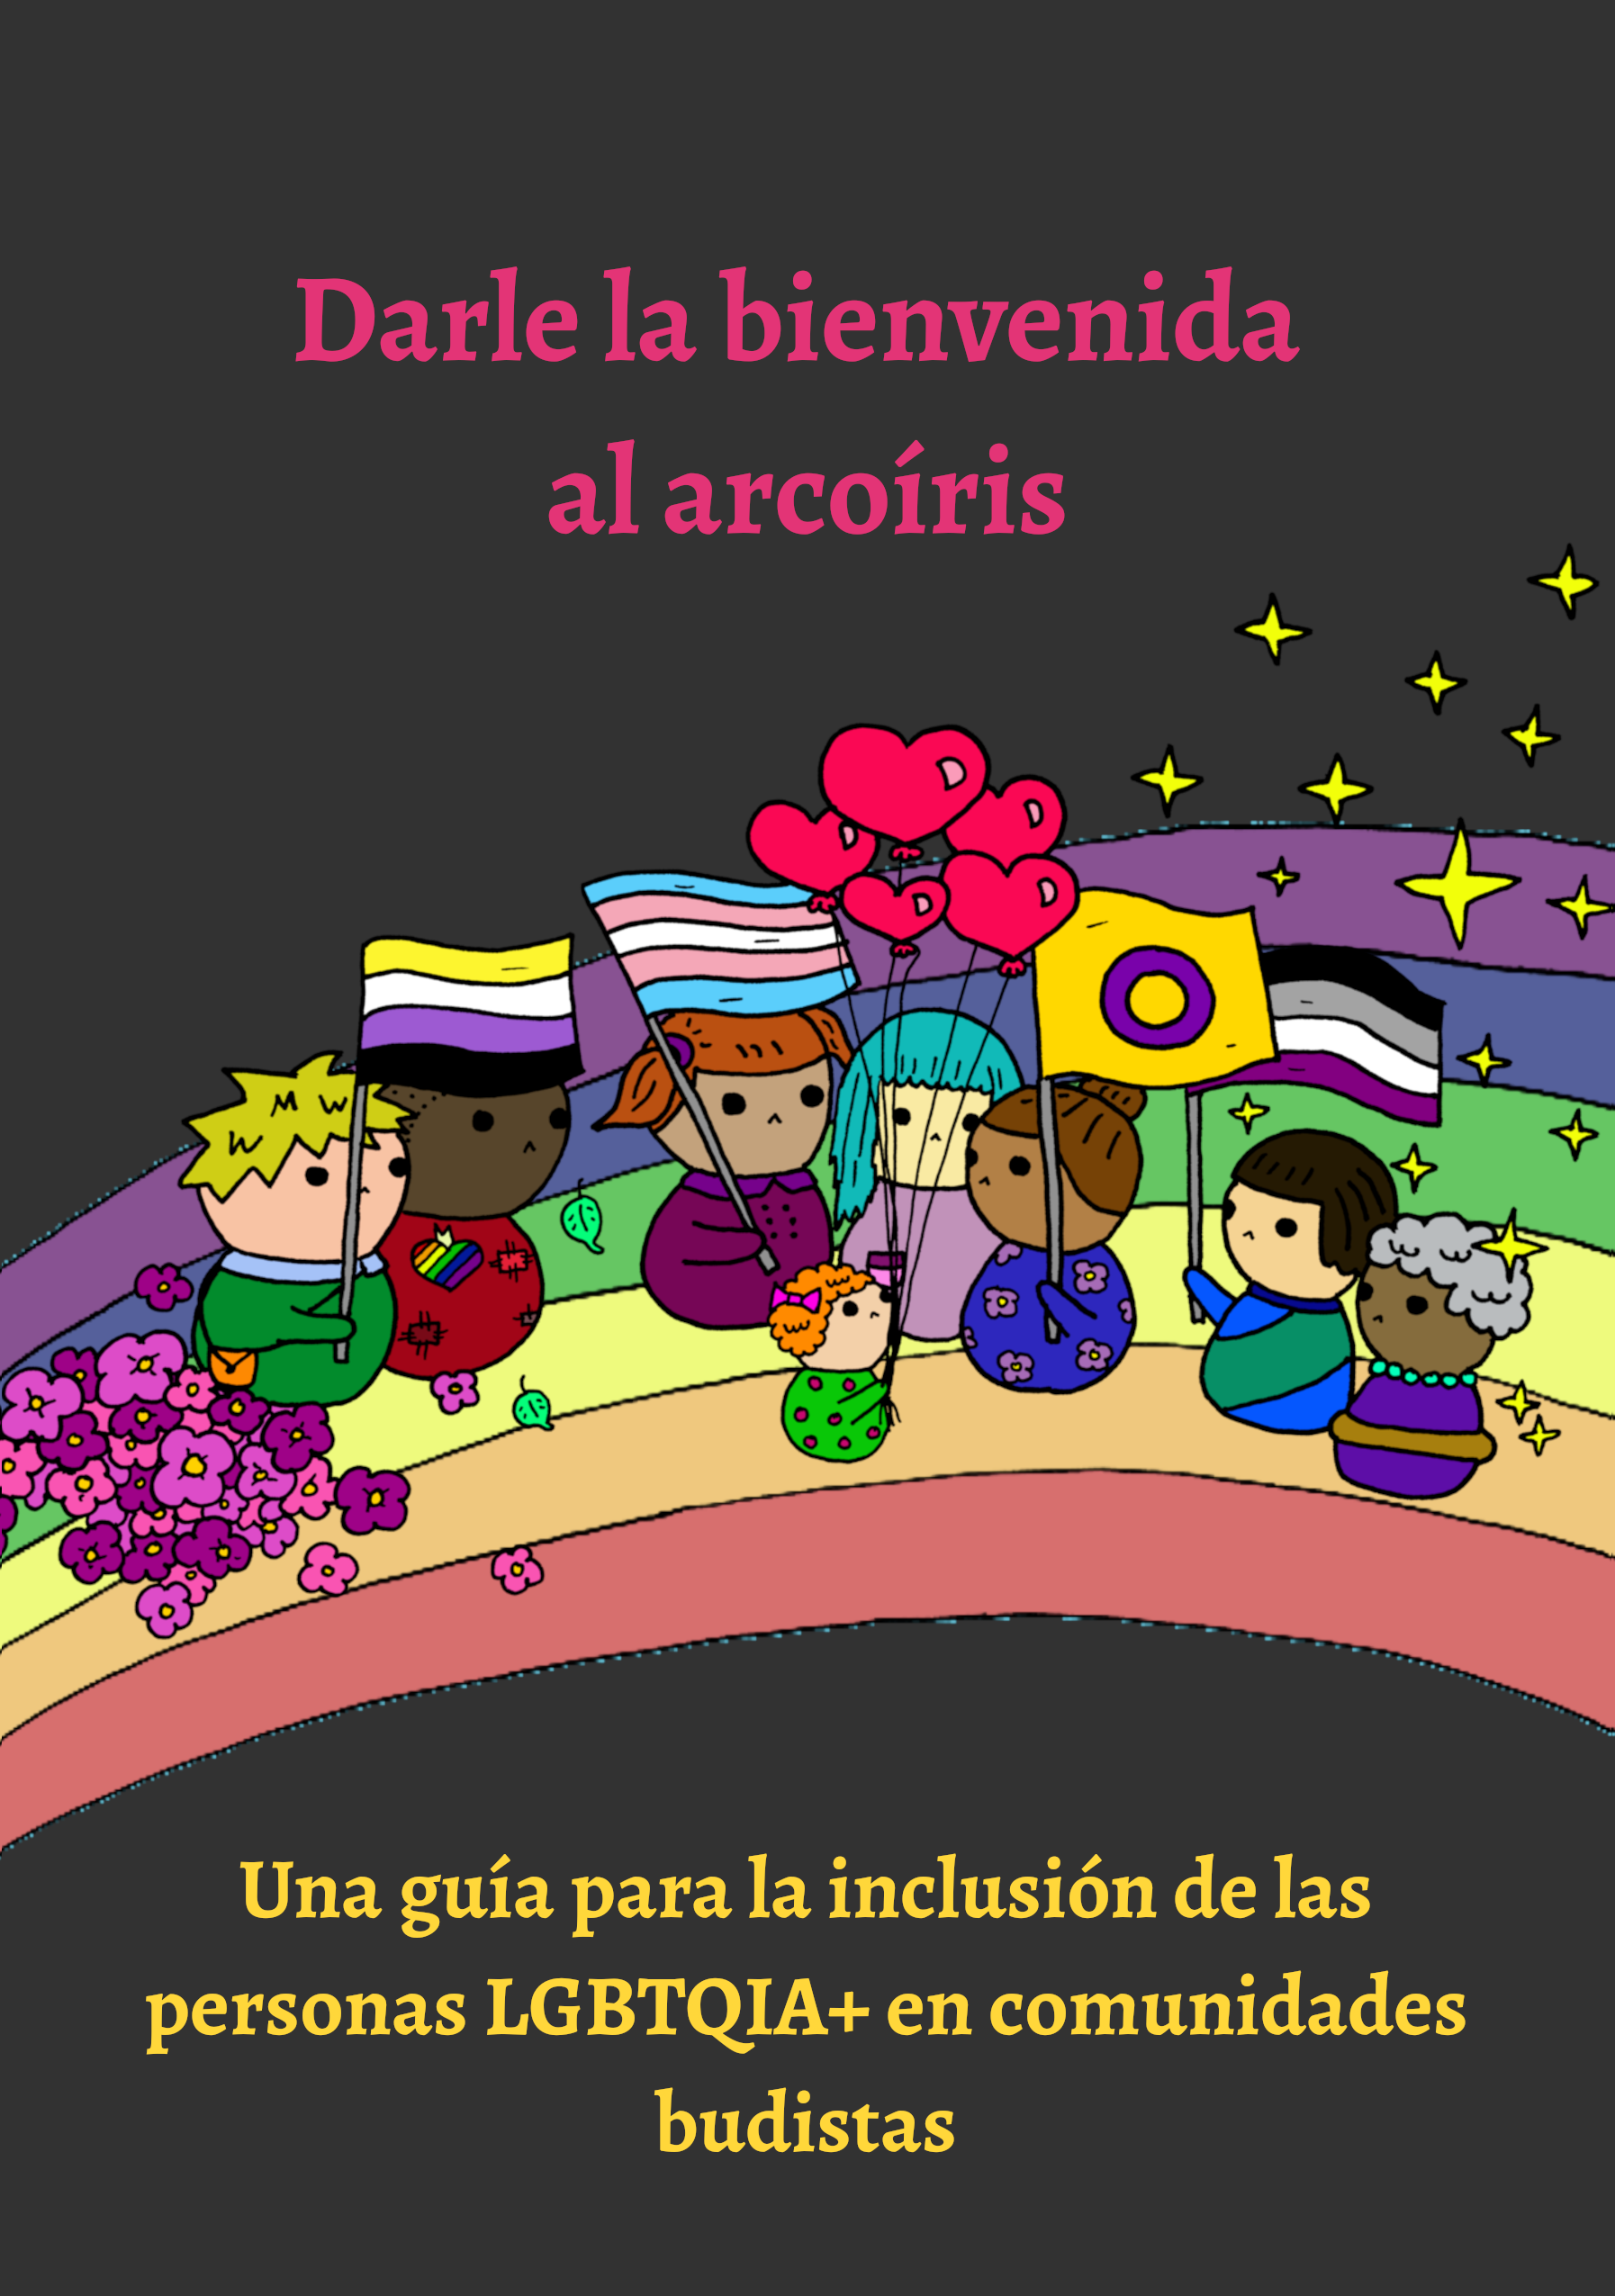
\includegraphics[width=\paperwidth]{front_espanol.png}}
\end{figure}

\restoregeometry

\begin{figure}[h]
    \makebox[150pt]{%
    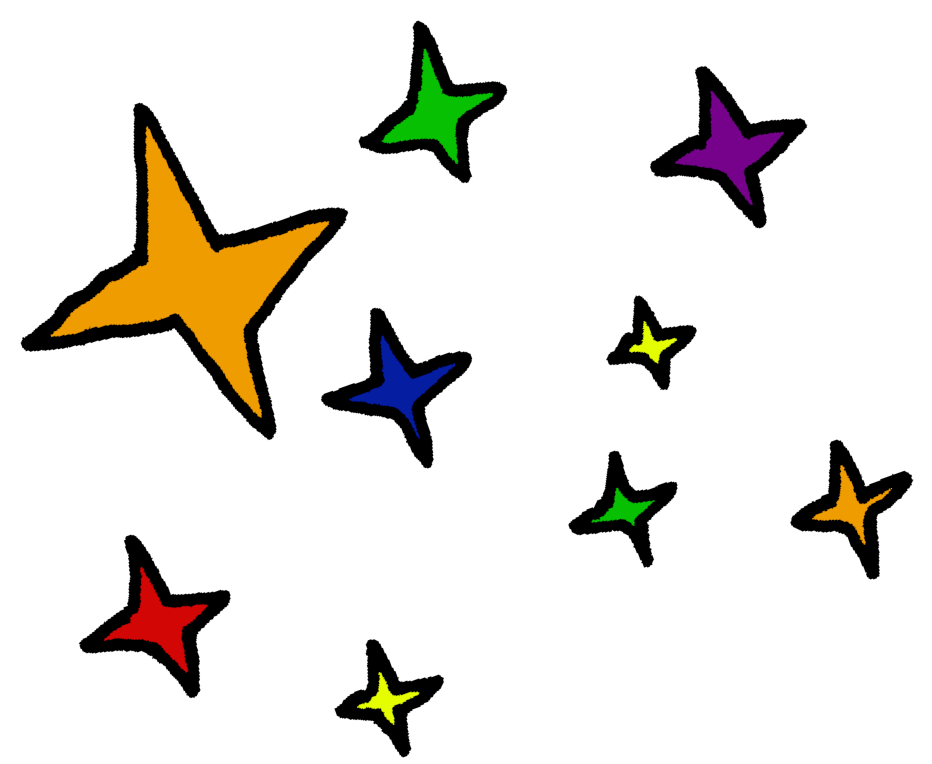
\includegraphics[width=0.4\paperwidth]{1.png}}
\end{figure}

\begin{center}

\thispagestyle{empty}

\sffamily
\color{orange}

\caps{\Huge \textbf{Darle la bienvenida al arcoíris}}

\medskip

\textit{ }
\color{violet}
\caps{\LARGE \textbf{Una guía para la inclusión personas LGBTQIA+ en comunidades budistas}}

\end{center}

\begin{figure}[h]
    \makebox[450pt]{%
    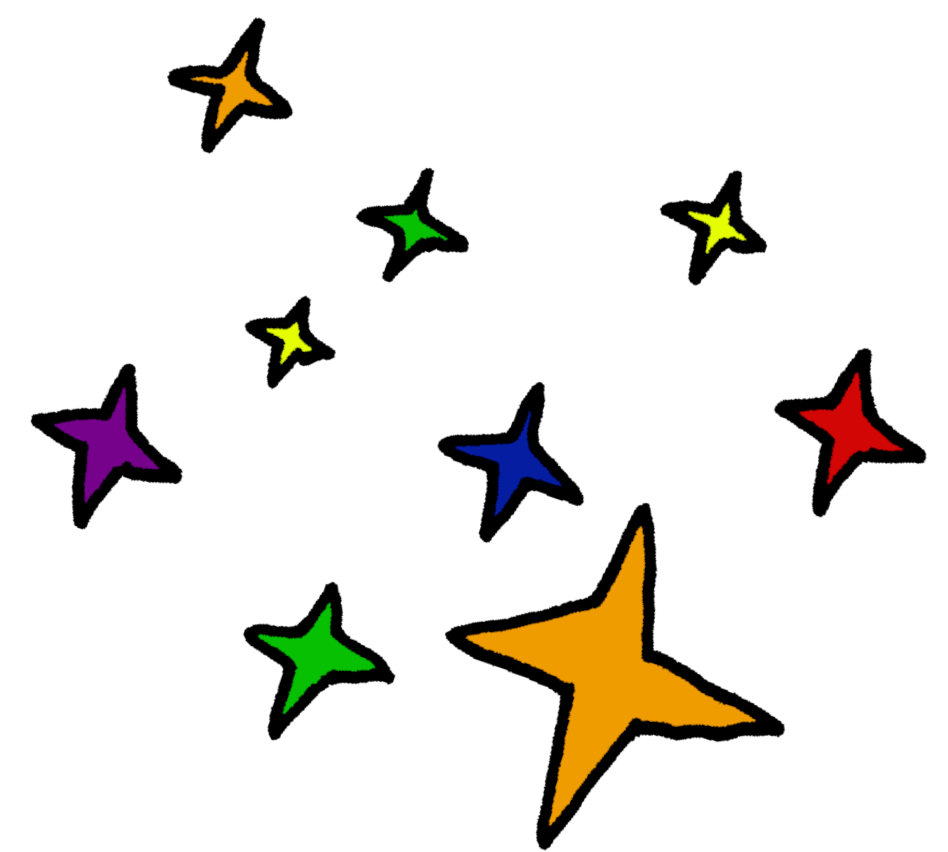
\includegraphics[width=0.4\paperwidth]{1c2.png}}
\end{figure}

\newpage
\thispagestyle{empty}
\mbox

\newpage
\thispagestyle{empty}
\mbox

\color{blue}
\tableofcontents
\thispagestyle{empty}
\markboth{}{}

\bigskip{}

\begin{figure}[h]
    \makebox[130pt]{%
    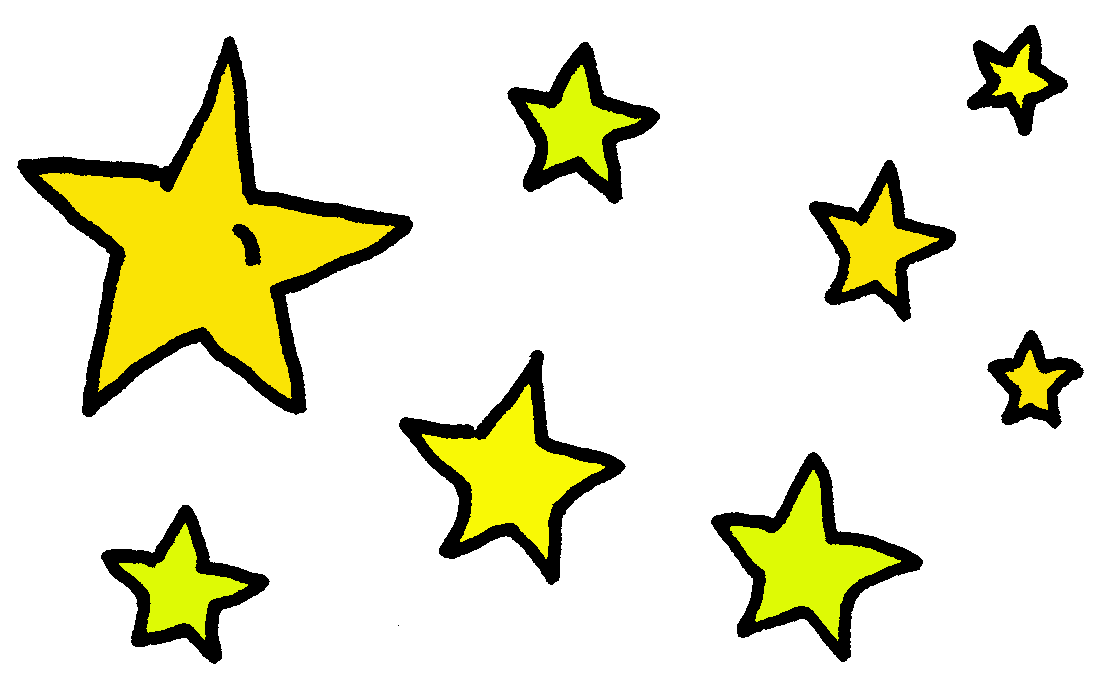
\includegraphics[width=0.4\paperwidth]{2.png}}
\end{figure}

\newpage
\thispagestyle{empty}

\rmfamily

\begin{center}\end{center}
\begin{center}

\vfill
\color{violet}
\caps{\LARGE \textit{\textbf{Que todos los seres sean felices}}}

\vfill

\end{center}

\begin{figure}[h]
    \centering
    \makebox[0pt]{%
    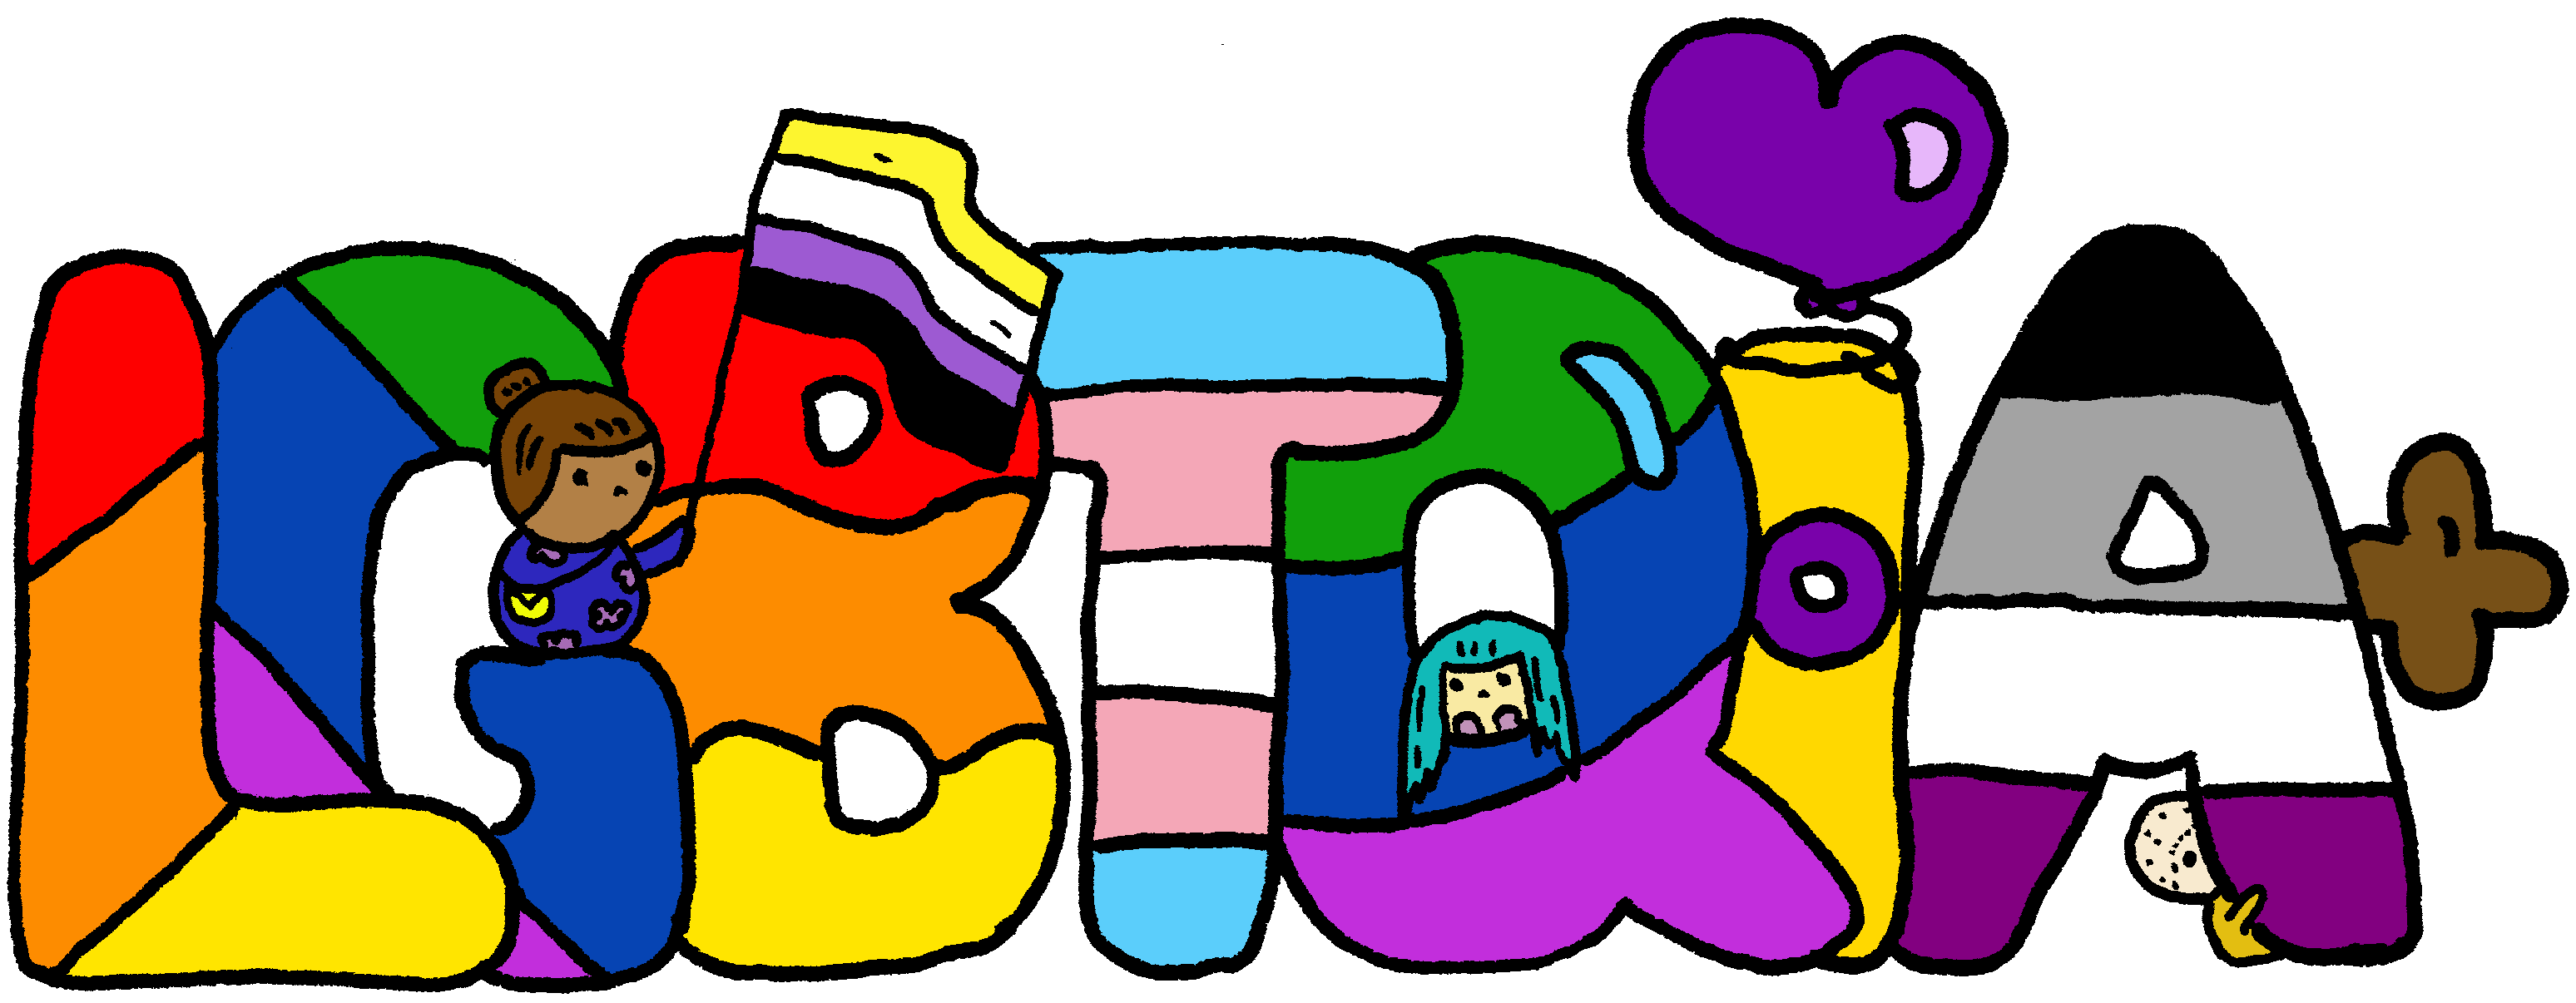
\includegraphics[width=0.8\paperwidth]{2-3.png}}
\end{figure}

\thispagestyle{empty}

\begin{figure}[h]
    \makebox[450pt]{%
    
\includegraphics[width=0.4\paperwidth]{2c2.png}}
\end{figure}

\thispagestyle{empty}

\mainmatter
\newpage
\thispagestyle{empty}

\begin{figure}[ht]
    \makebox[250pt]{%
    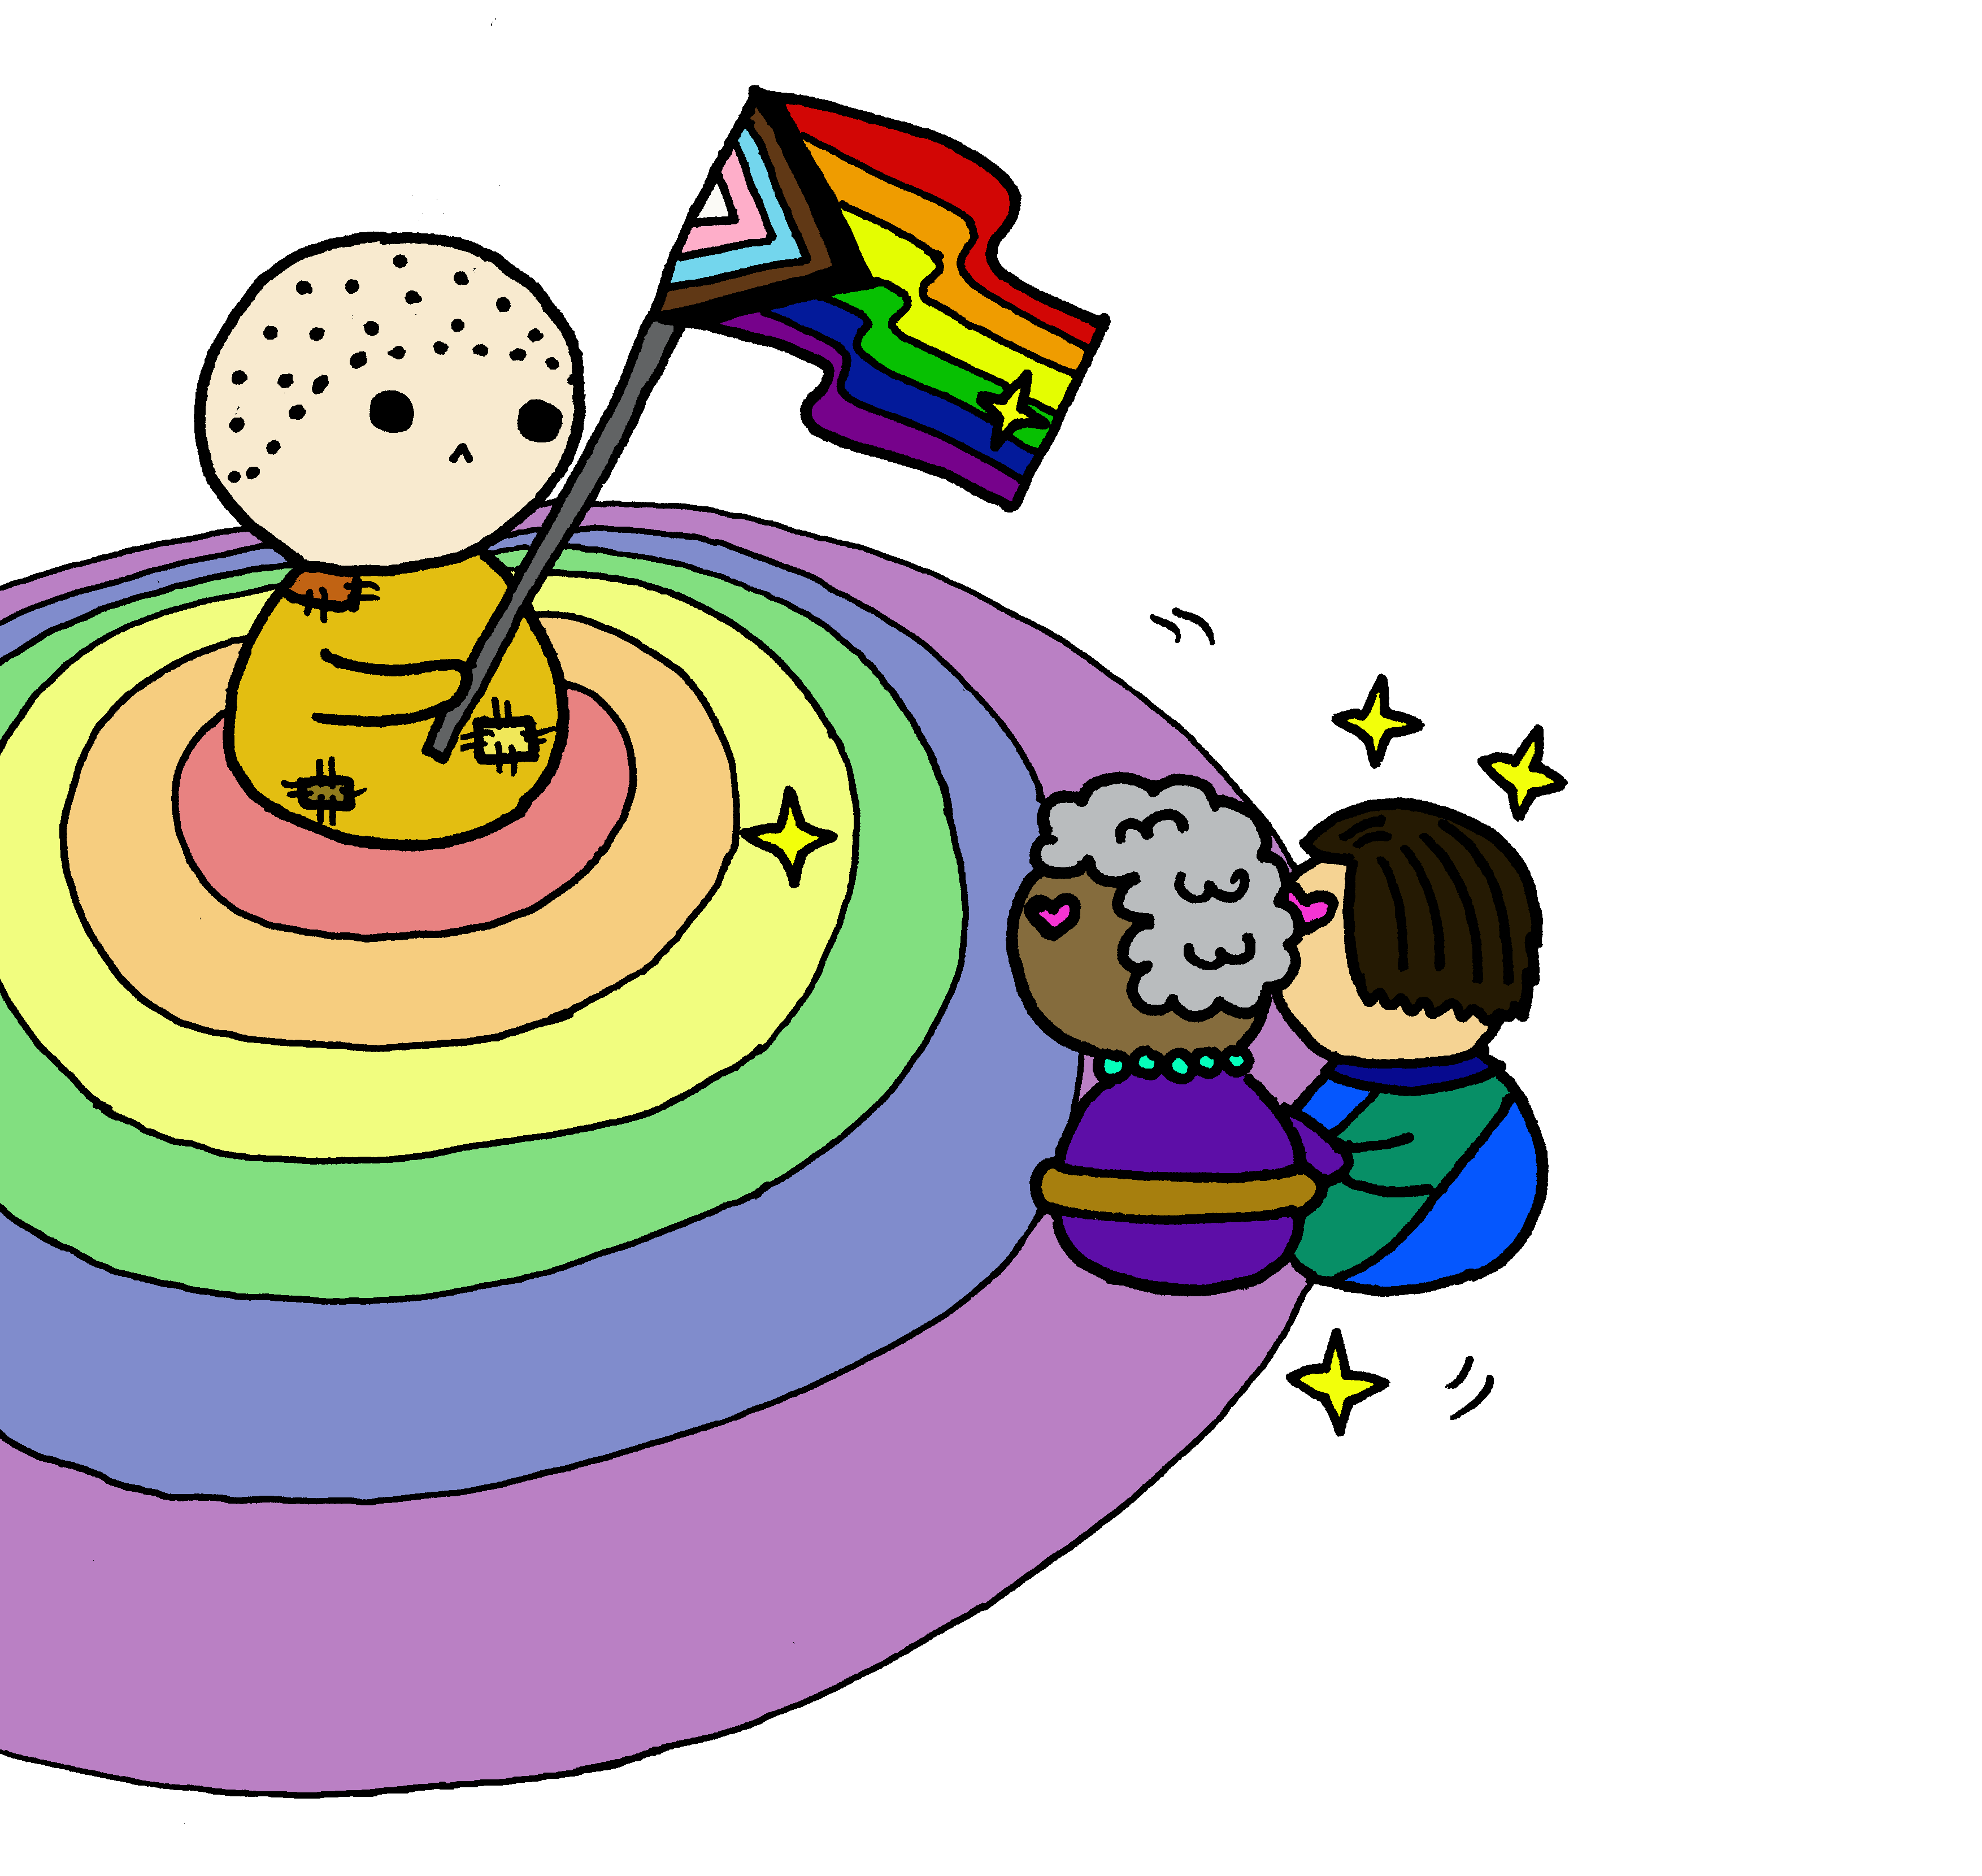
\includegraphics[width=0.8\paperwidth]{4.png}}
\end{figure}

\color{purple}
\begin{quote}
\centering
\doublespacing
\textit{\Large \textbf{Juntes, podemos hacer que nuestros centros budistas sean lugares más seguros e inclusivos para nuestra comunidad arcoíris.}}
\end{quote}

\newpage
\thispagestyle{empty}

\begin{quote}
\doublespacing
\centering
\textit{\Large \textbf{Al perpetuar la homofobia, la bifobia, la transfobia y la interfobia, las personas u organizaciones budistas perpetúan también el odio, la violencia y el abuso.}}
\end{quote}

\begin{figure}[h]
    \centering
    \makebox[0pt]{%
    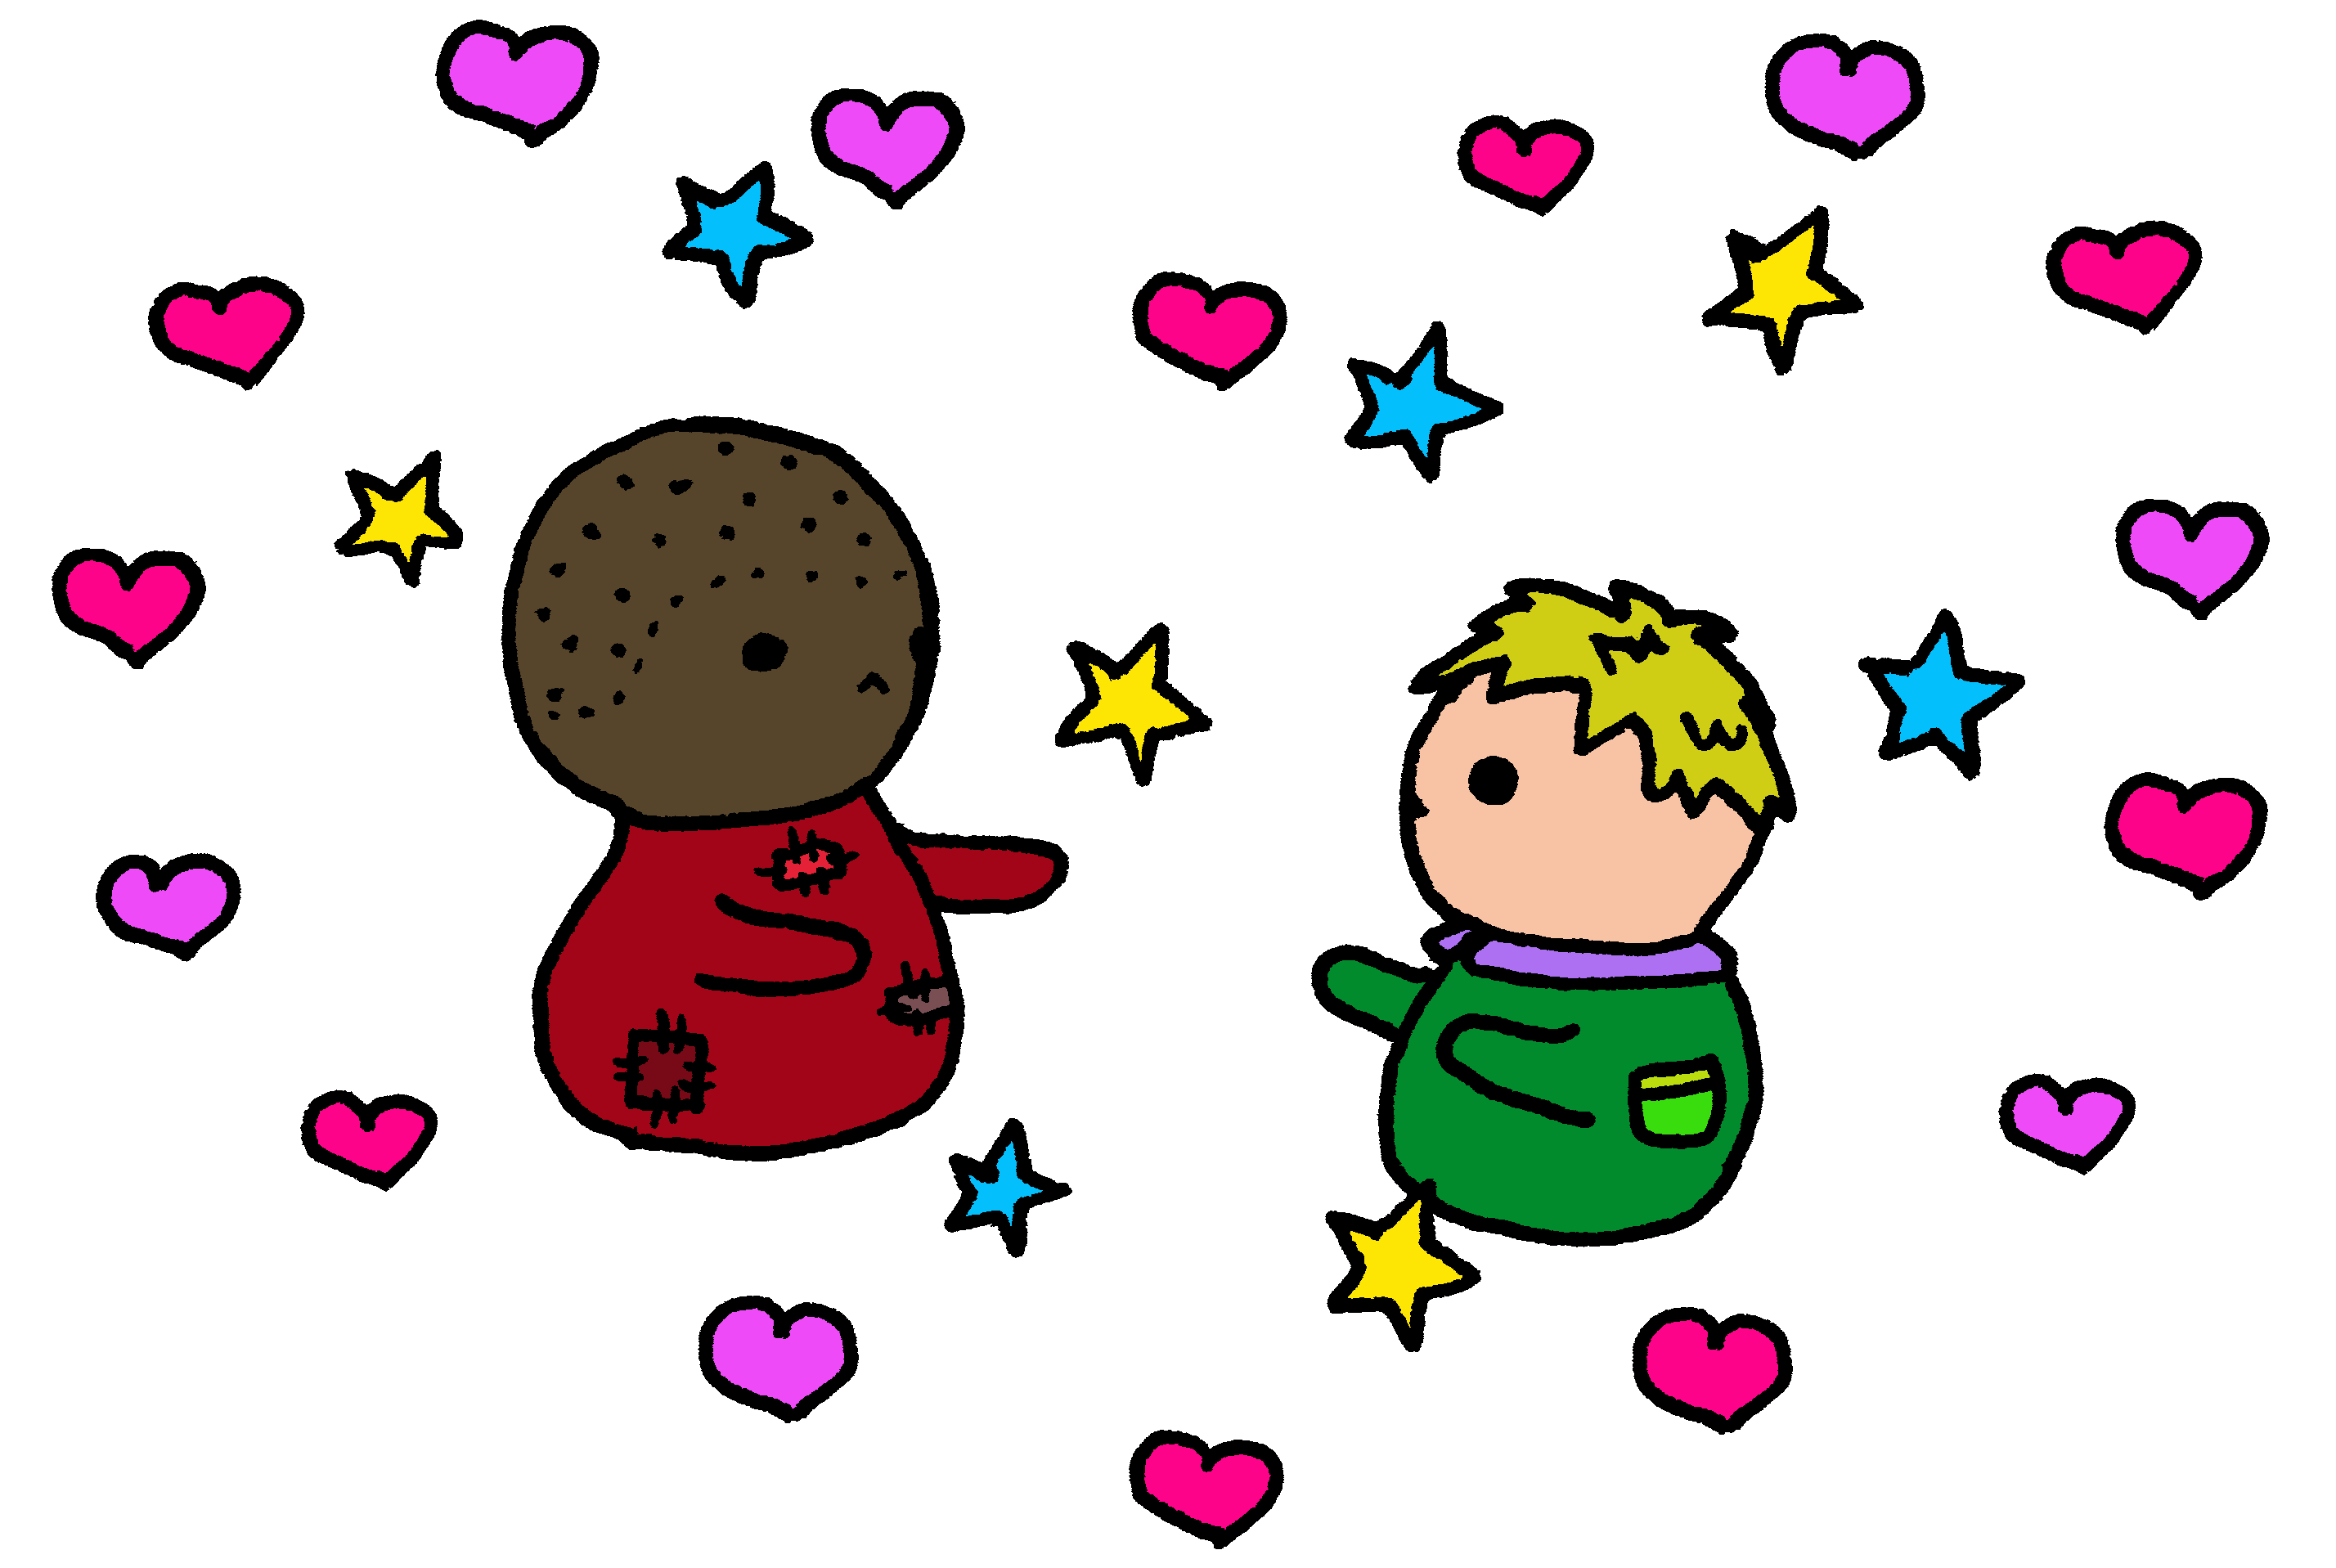
\includegraphics[width=0.6\paperwidth]{6-7.png}}
\end{figure}

\begin{quote}
\centering
\doublespacing
\textit{\Large \textbf{Comprender cómo las personas y las organizaciones pueden ser más acogedoras e inclusivas con les budistas LGBTQIA+ nos ayudará a practicar genuinamente el amor bondadoso y la compasión hacia todes en nuestra comunidad.}}
\end{quote}

\color{darkgray}
\setlength{\parindent}{15pt}
\chapter*{Nota del equipo de traducción al español}
\addcontentsline{toc}{chapter}{Nota del equipo de traducción al español}

Debido a las diferencias gramaticales y lingüísticas entre el inglés y el español, hemos decidido hacer uso del lenguaje no binario directo (LND) con la -e como morfema de género para reemplazar al masculino genérico tradicional. Así, el texto se mantiene incluyente para todos, todas y todes. Presentamos a continuación una explicación del LND para facilitar la lectura del librillo a quienes lo necesiten.

A pesar de argumentarse de que se trata de una `imposición' lingüística de la última década, el uso del morfema -e en español tiene sus orígenes en la propuesta de Álvaro García Meseguer (1976) para solucionar los problemas que el masculino genérico pueda crear, como la ambivalencia semántica y la ocultación de la mujer. El masculino genérico oculta, además, a las personas no binarias (véase `Información sobre la comunidad LGBTQIA+' al final de este librillo). Por ello, el uso del morfema de género -e ha ganado popularidad para crear un lenguaje no sexista e inclusivo, y forma ya parte de ciertas palabras como `cantante' o `alegre'. El LND es fácil de usar, leer y comprender. En palabras de Meseguer:

\begin{itemize}
\setlength\itemsep{-0.3em}
  \item Como las desinencias en o y en a son, en la mayoría de los casos, las propias del masculino y el femenino, una solución sencilla consiste en asignar la desinencia en e al género común, es decir, a la persona.
  \item Así, cuando une se dirija a un grupo en una conferencia, en una carta circular, etc., podrá comenzar diciendo `querides amigues'.
\end{itemize}

Es decir, en el LND cambiamos el morfema -o del masculino genérico por el morfema -e, tanto en sustantivos plurales como en adjetivos que hacen referencia a un grupo de personas de distintos géneros. Así, en lugar de decir `todos', `amigos' o `maestros', podemos decir `todes', `amigues' y `maestres'. En el caso de las palabras que ya terminan en -e y no son neutras, como `señores' o `autores', le traductore Ártemis López propone el uso de artículos previo a dichas palabras; tendríamos así `les señores' y `les autores'.

Hemos decidido usar el LND puesto que conlleva un cambio en la lengua y, en consecuencia, la mentalidad de todes para crear así una sociedad más inclusiva y equitativa. Como menciona Meseguer:

\begin{itemize}
\setlength\itemsep{-0.3em}
  \item La lengua, resultado de los hábitos culturales del pasado, condiciona la estructura mental de los hablantes y, con ello, también los hábitos culturales futuros. Tremendo círculo vicioso: el idioma es sexista porque la sociedad lo ha sido y la sociedad será sexista porque el idioma lo es.
  \item En este terreno, cada día son más las personas empeñadas en llevar adelante una revolución cultural. Pero ésta no será posible sin transformar profundamente el idioma. Ambas revoluciones deben andar parejas.
\end{itemize}

\textit{Ngakpa Alan Serrato Martínez (Tenzin Dradul)} \\
\textit{Grégory Touche (Ngakpa Padma Özer)} \\
\textit{David Santamarina (Kansei)}

\begin{figure}[h]
    \centering
    \makebox[0pt]{%
    
\includegraphics[width=0.6\paperwidth]{Guide_color.png}}
\end{figure}

\chapter*{Darle la bienvenida al Arcoiris}
\addcontentsline{toc}{chapter}{Darle la bienvenida al Arcoiris}
% \markboth{Darle la bienvenida al arcoíris}{Darle la bienvenida al Arcoiris}

\begin{wrapfigure}{hl}{0.25\textwidth}
    \makebox[150pt]{%
    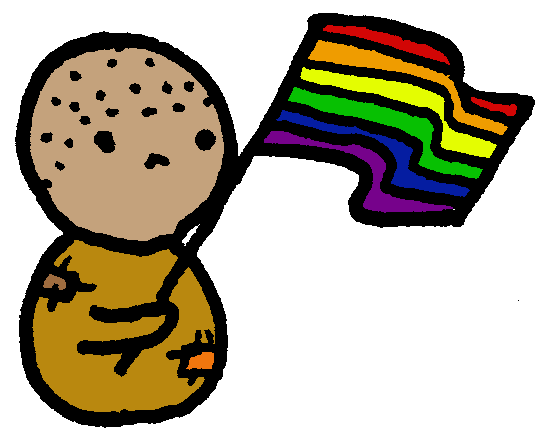
\includegraphics[width=0.25\textwidth]{2c3.png}}
\end{wrapfigure}
La comunidad budista Rainbodhi LGBTQIA+ creó este librillo para proporcionar consejos prácticos sobre cómo ayudar a que los templos, monasterios y organizaciones budistas sean espacios seguros e inclusivos para les budistas LGBTQIA+.

\phantomsection
\section*{La sigla del arcoíris}
\addcontentsline{toc}{section}{La sigla del arcoíris}

La sigla `LGBTQIA+' significa Lesbiana, Gay, Bisexual, Trans, Queer, Intersexual, Asexual, y el signo `+' representa a otras identidades posibles. Este término tiene por nombre `sigla del arcoíris' porque nuestra comunidad está conformada por muchos grupos distintos, tal y como un arcoíris está conformado por muchos colores.

El término `LGBTQIA+' abarca una gran diversidad de identidades, incluidas las características físicas, la orientación sexual y las identidades de género. Estos grupos son bastante diferentes entre sí, pero a veces se pueden yuxtaponer. Por ejemplo, los términos `lesbiana', `gay' y `bisexual' son orientaciones sexuales; el término `transgénero' se refiere a la identidad de género; `queer' puede referirse tanto a la identidad de género como a la sexualidad; `intersexual' se refiere a las personas que nacen con características físicas tanto femeninas como masculinas; `asexual' se refiere a una ausencia de sexualidad. También puede existir muchas combinaciones de estos aspectos.

A pesar de que hay diversas identidades dentro de la comunidad LGBTQIA+, todas comparten desafíos comunes como los prejuicios, la discriminación, los obstáculos legales y la violencia, solo por ser elles mismes.

\phantomsection
\section*{Hacer el cambio juntes}
\addcontentsline{toc}{section}{Hacer el cambio juntes}

Las personas LGBTQIA+ a menudo se enfrentan al rechazo y a la opresión por parte de la sociedad y de comunidades religiosas.
Frecuentemente, El Buda habló en contra de la discriminación y dijo que todos los seres sintientes merecían amor sin distinción alguna. Ya que todes somos capaces de alcanzar la iluminación, debemos asegurarnos de no excluir a nadie en nuestras comunidades budistas.

No siempre somos conscientes de que nuestras organizaciones, templos y centros de retiro budistas no son necesariamente lugares acogedores para la comunidad LGBTQIA+, y
es posible que muchas personas no entiendan que sus acciones y sus palabras pueden dañar a las personas de la comunidad LGBTQIA+. Puede que las organizaciones no se den cuenta de cómo excluyen a las personas pertenecientes a esta comunidad.

La buena noticia es que todo esto está cambiando, y podemos ser parte de ese cambio.

\phantomsection
\section*{Escucha a la comunidad LGBTQIA+}
\addcontentsline{toc}{section}{Escucha a la comunidad LGBTQIA+}

\begin{wrapfigure}{l}{0.15\textwidth}
    \centering
    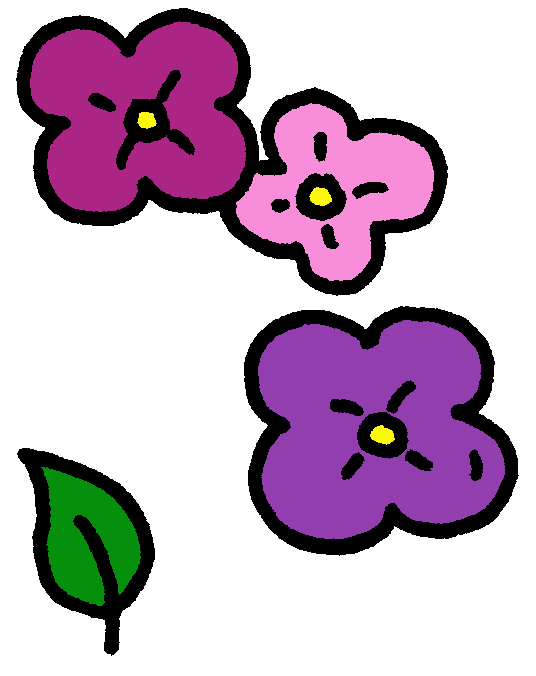
\includegraphics[width=0.15\textwidth]{2c4.png}
\end{wrapfigure}

Es fundamental escuchar la voz de les budistas LGBTQIA+ para entender sus experiencias. Un estudio reciente patrocinado por Rainbodhi y dirigido por el Dr. Stephen Kerry de la Universidad Charles Darwin (Australian LGBTQIA+ Buddhists Research Project, Darwin 2020),  descubrió que las comunidades budistas australianas pueden ser entornos difíciles para les budistas LGBTQIA+. Con respecto a los centros budistas que frecuentan, les encuestades informaron lo siguiente:

\begin{itemize}
\setlength\itemsep{-0.3em}
  \item El 61\% intió que los centros budistas ignoran o invisibilizan a la comunidad LGBTQIA+ y sus desafíos
  \item El 55\% ha estado inseguro de revelar su identidad LGBTQIA+
  \item El 54\% ha atestiguado actos o comentarios sexistas
  \item El 37\% ha atestiguado actos o comentarios homófobos
  \item El 26\% ha atestiguado actos o comentarios transfóbicos
  \item El 26\% ha atestiguado actos o comentarios racistas
  \item El 16\% de les encuestades le dijeron que su identidad LGBTQIA+ era incompatible con las enseñanzas budistas.
\end{itemize}

Estos resultados muestran que los centros budistas no siempre son espacios seguros para budistas LGBTQIA+. Reconocer la existencia de los prejuicios y la discriminación es un primer paso importante para llevar a cabo los cambios necesarios para crear más comunidades budistas seguras e inclusivas.

\phantomsection
\section*{El budismo tiene un pasado (y futuro) LGBTQIA+}
\addcontentsline{toc}{section}{El budismo tiene un pasado (y futuro) LGBTQIA+}

Las personas gay, trans e intersexuales siempre han existido en la historia de la humanidad; también son espirituales, por lo que no es de sorprenderse que el budismo tenga un pasado relacionado a esta comunidad.

Los antiguos textos budistas tratan sobre la atracción por el mismo sexo y la sexualidad sin ningún tinte de juicio moral o negatividad, y hay también relatos de laicos y monjes/monjas que han cambiado de género. La antigua sociedad india reconocía una categoría de personas que no se consideraban ni hombres ni mujeres, a quienes hoy en día podríamos denominar `transgénero' o `personas de tercer género', y otra categoría de personas que tenían características sexuales tanto masculinas como femeninas, a las que quizás nos podríamos referir hoy como `intersexuales'. Algunos de estos grupos han sido estigmatizados y han sufrido adversidades sociales a lo largo de la historia del budismo, y para algunos de ellos, esta discriminación continúa a día de hoy.

\subsubsection*{El Orgullo LGBTQIA+ en el budismo}

Las personas de la comunidad LGBTQIA+ han participado en el desarrollo del budismo como adeptos al monasticismo, seguidores láiques, profesores, investigadores y académiques. Sin embargo, sus historias a menudo caen en el olvido y sus experiencias, en el silencio. Ya que, en general, la sociedad ha comenzado a comprender y aceptar más a la comunidad LGBTQIA+, estamos en el momento indicado para que les practicantes y organizaciones budistas  celebren nuestra comunidad arcoíris y muestren su apoyo de una manera concreta. De esta forma, las personas de la comunidad LGBTQIA + podrán estar seguras de que se les considerará como parte íntegra de la comunidad budista en el futuro.

\begin{figure}[h]
    \centering
    \makebox[0pt]{%
    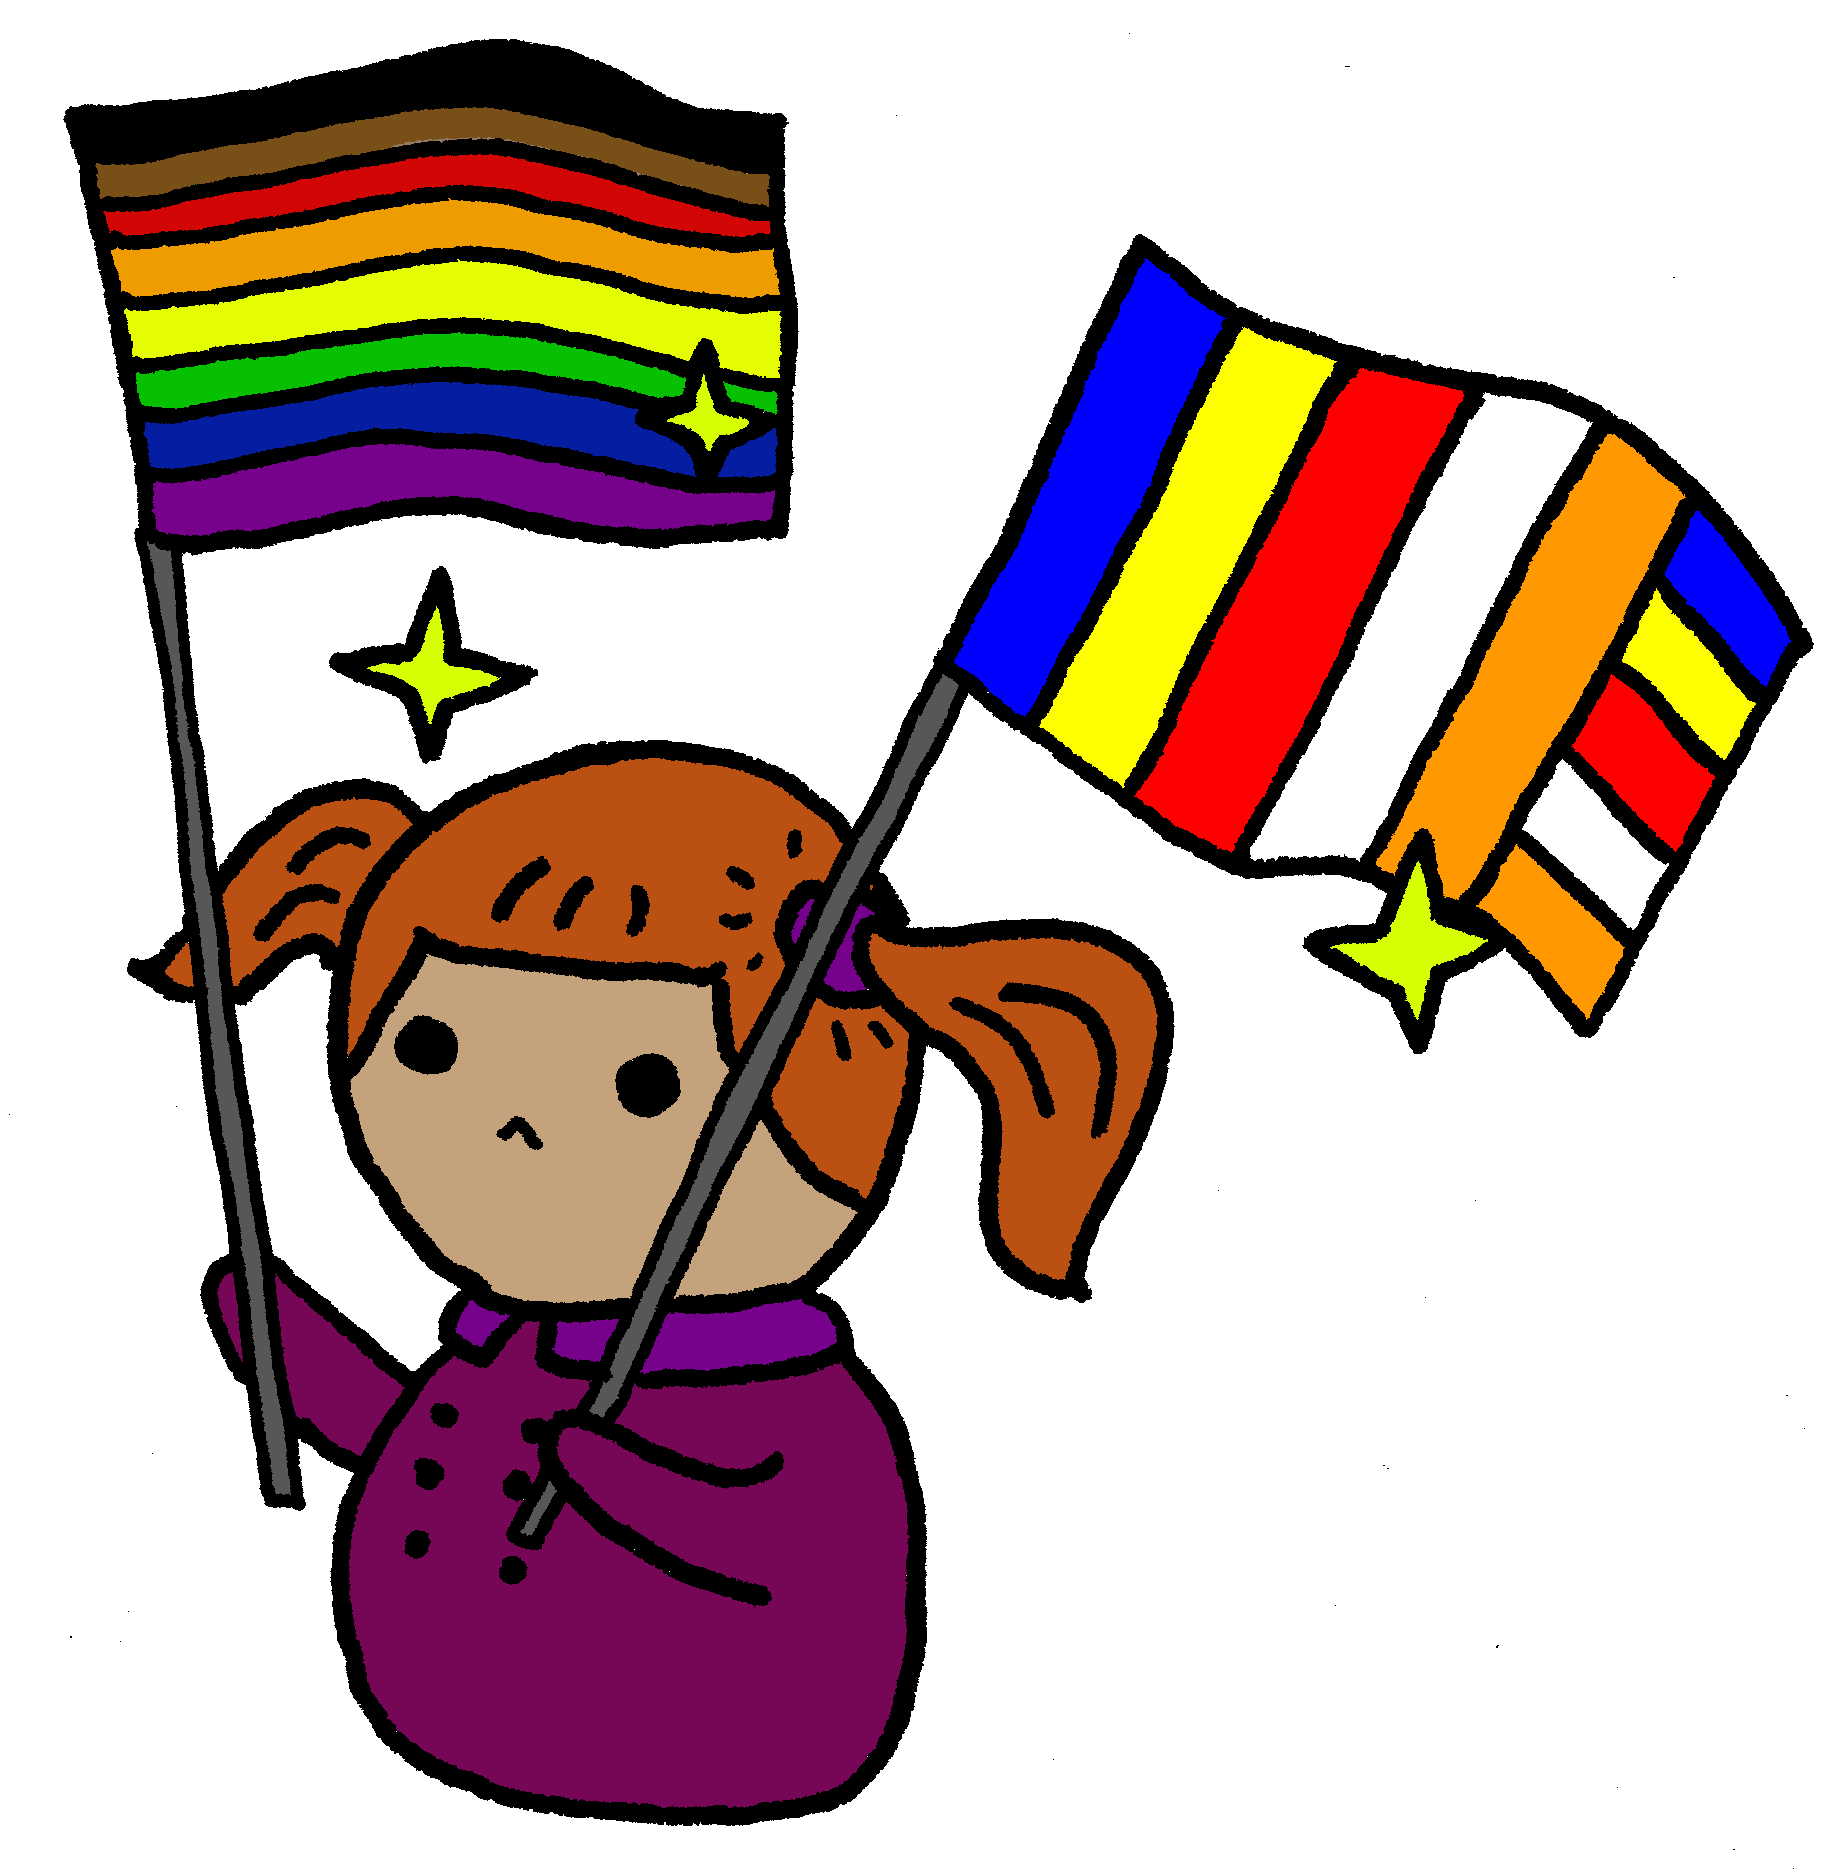
\includegraphics[width=0.4\paperwidth]{9.png}}
\end{figure}

\begin{quote}
\centering
\doublespacing
\textit{\Large \textcolor{purple}{\textbf{Todes, independientemente de su género y sexualidad, merecen vivir sin miedo a ser rechazades y estar orgulloses de quiénes son.}}}
\end{quote}

\newpage
\thispagestyle{empty}

\begin{figure}[h]
    \centering
    \makebox[0pt]{%
    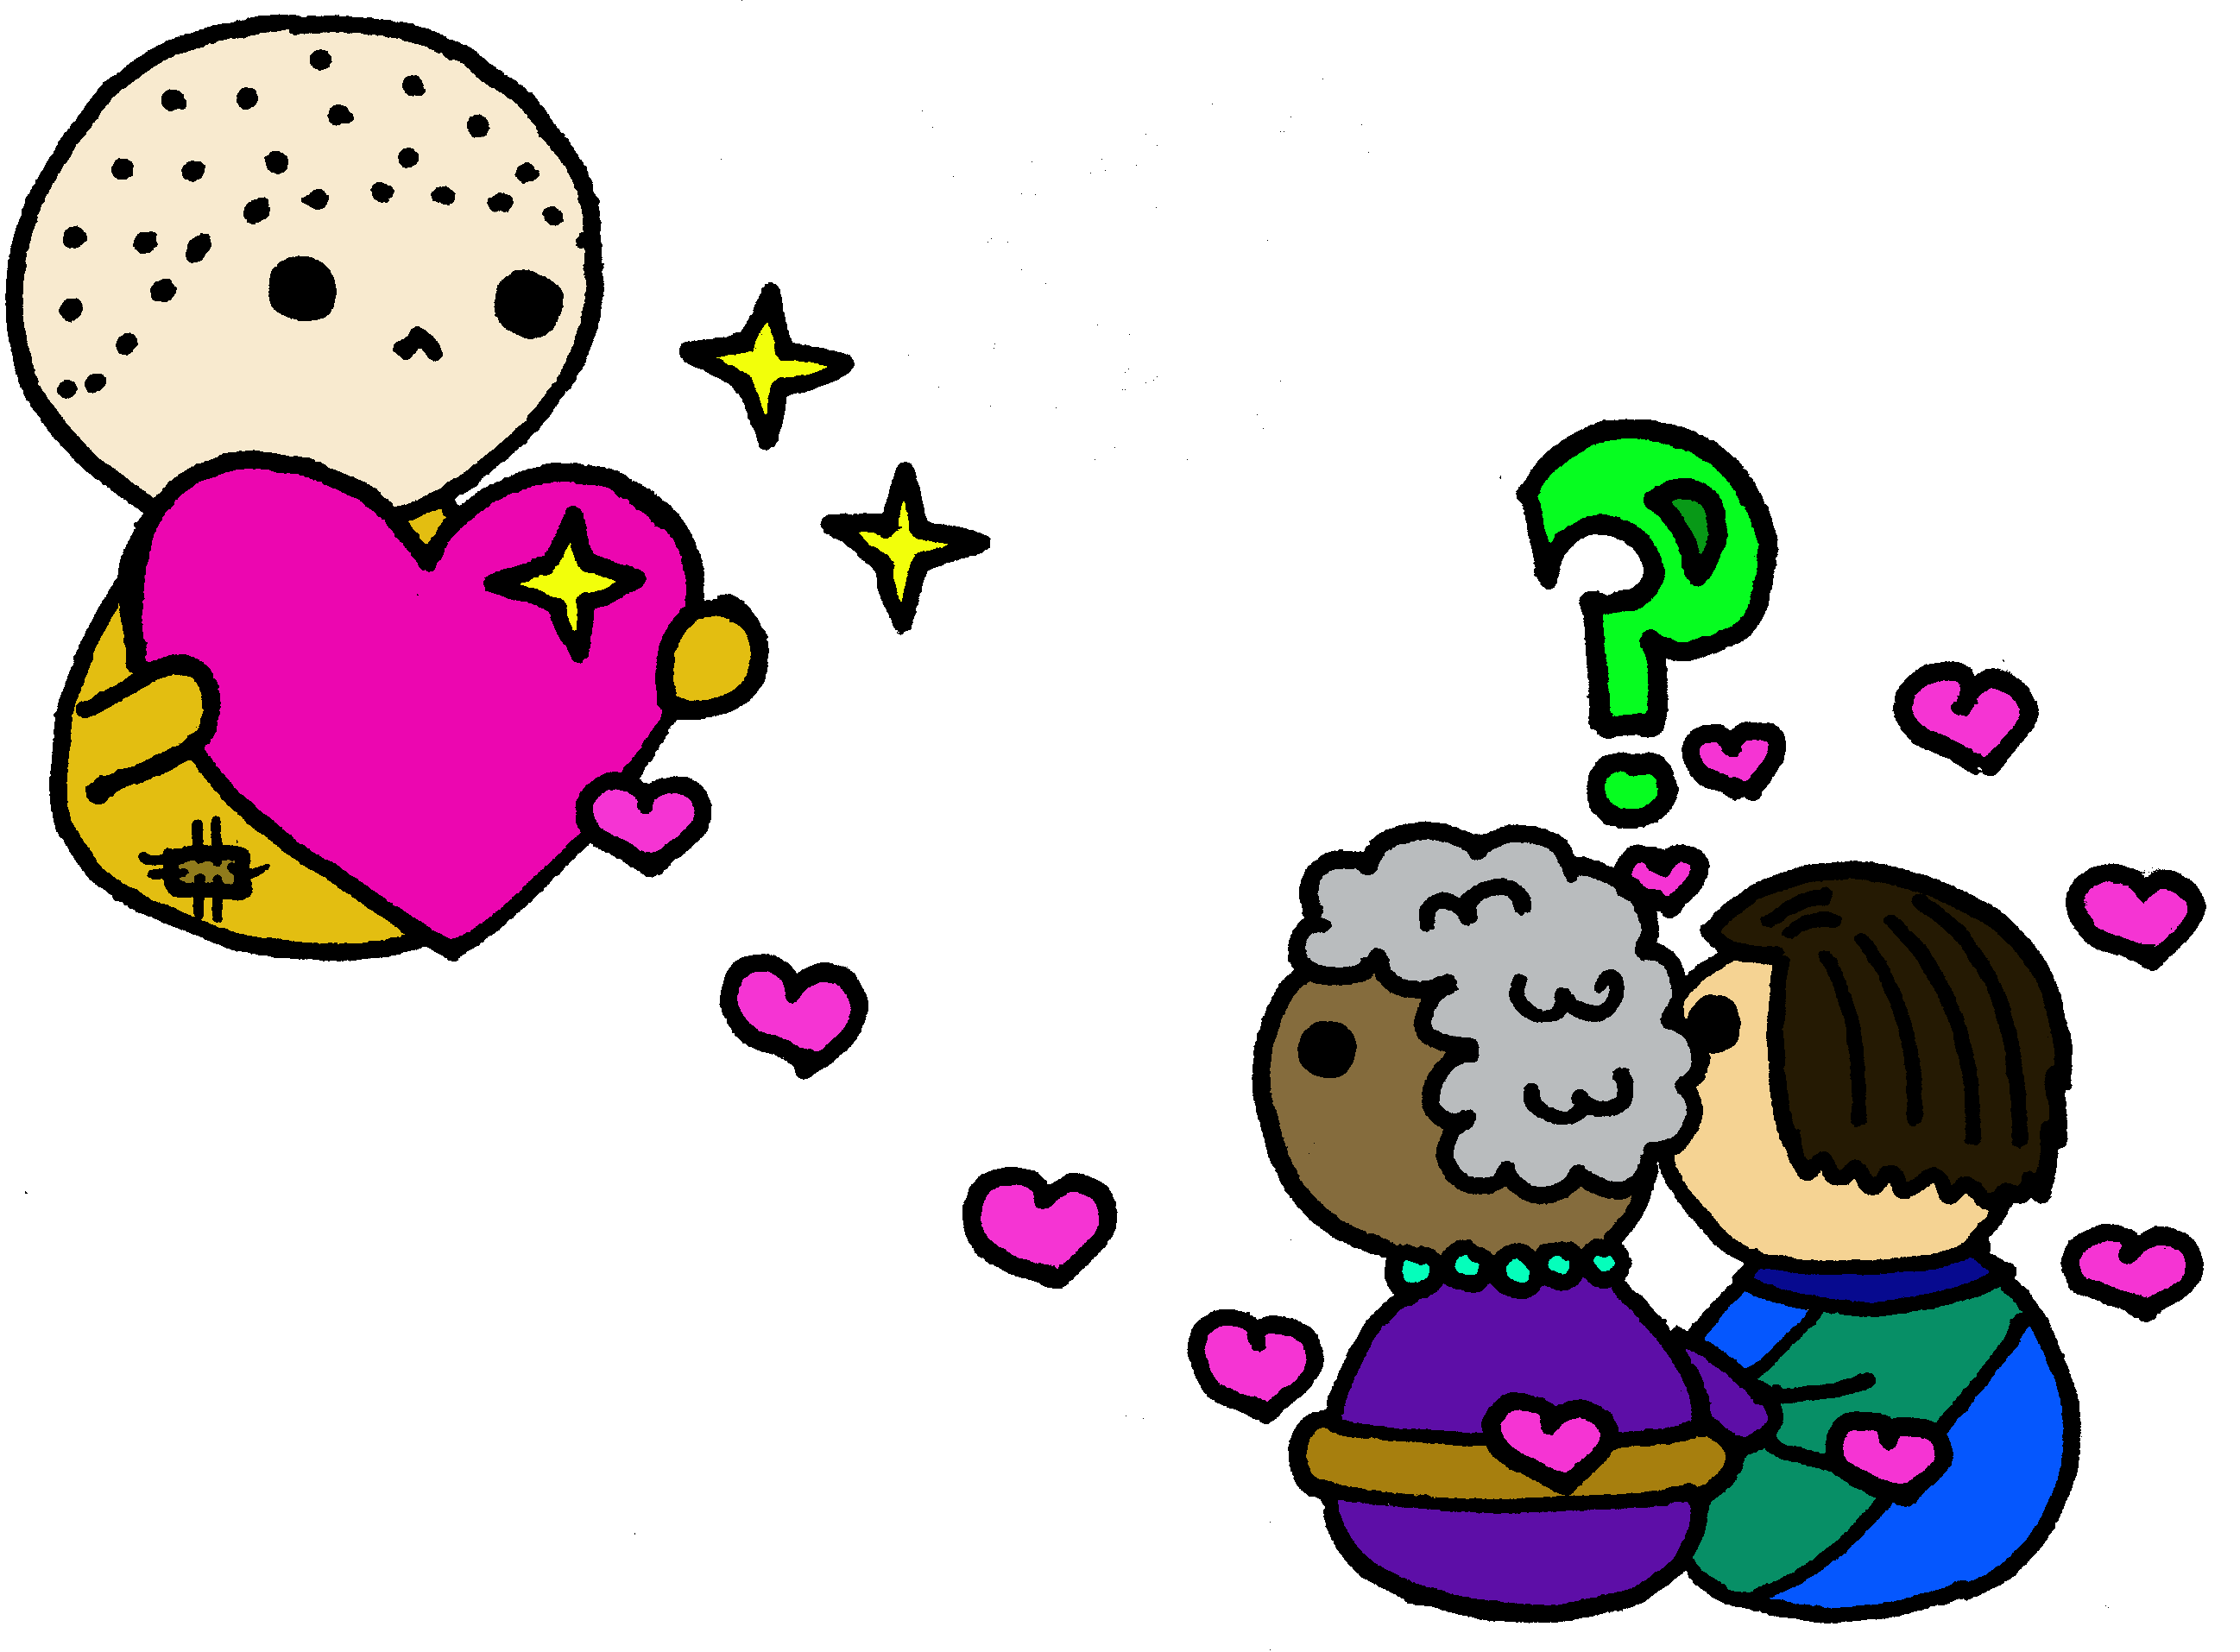
\includegraphics[width=0.9\paperwidth]{10.png}}
\end{figure}

\begin{quote}
\centering
\doublespacing
\textit{\Large \textcolor{orange}{\textbf{Las buenas amistades son la totalidad del camino espiritual.}}}
\end{quote}

\chapter*{Sé une amigue espriritual de les budistas LGBTQIA+}
\addcontentsline{toc}{chapter}{Sé une amigue espriritual de les budistas LGBTQIA+}
% \markboth{Darle la bienvenida al arcoíris}{Sé une amigue espriritual de les budistas LGBTQIA+}

\phantomsection
\section*{Sé una persona aliada}
\addcontentsline{toc}{section}{Sé una persona aliada}

Ser une amigue espiritual es una parte importante de ser budista; al ser une aliade de la comunidad LGBTQIA+ y al alzar la voz por les demás  puedes ayudar a que otres se sientan segures y bienvenides.

Una persona aliada es aquella que apoya los derechos de la comunidad LGBTQIA+ y que lucha activamente en contra la homofobia, la bifobia y la transfobia. Les aliades tienden a ser heterosexuales y/o cisgénero (personas que se identifican con el sexo que se les asignó al nacer).

Las personas aliadas reconocen los obstáculos que experimentan las personas LGBTQIA+ y, por lo tanto, usan su privilegio para contrarrestar la discriminación que sufre esta comunidad. Une aliade puede también ser alguien que pertenezca a la comunidad LGBTQIA + y apoye una disidencia de la cual no formen parte. Por ejemplo, un hombre gay cisgénero puede ser un aliado de las personas transgénero, o una persona intersexual podría apoyar los derechos de las personas atraídas por su mismo sexo.

Las personas aliadas ayudan a las personas LGBTQIA + a explicar los problemas que experimentan en el mundo. Para ser una buena persona aliada, primero es importante escuchar a las personas LGBTQIA+ y aprender sobre sus experiencias diversas, lo cual implica aprender algunas nociones básicas: qué significan las letras de la sigla del arcoíris, la diferencia entre sexualidad y género, saber que los problemas que sufren las personas trans son diferentes a los problemas sufren las personas LGB, cuáles son los derechos humanos por los que luchan las personas intersexuales… Todes podemos ser une aliade de les demás, independientemente de su sexualidad o género.

\begin{figure}[h]
    \centering
    \makebox[0pt]{%
    
\includegraphics[width=0.5\paperwidth]{12.png}}
\end{figure}

\begin{quote}
\centering
\doublespacing
\textit{\Large \textcolor{orange}{\textbf{Ser une aliade es un acto de amistad y compasión}}}
\end{quote}

\phantomsection
\section*{Promueve la inclusión}
\addcontentsline{toc}{section}{Promueve la inclusión}

Es importante recordar que ya hay personas LGBTQIA+ en las comunidades budistas. Nunca debemos asumir que todes son heterosexuales ni que podemos saber el género o los pronombres de alguien basándonos en su apariencia física. Reconocer que las personas LGBTQIA+ están presentes en nuestros templos, retiros y centros es el primer paso para encarnar la inclusión.

Frecuentemente, las personas LGBTQIA+ han sido invisibilizadas en las comunidades budistas, y sus necesidades específicas no han sido reconocidas ni atendidas. A veces, no pueden mencionar sus identidades porque temen el rechazo y pueden sentirse incómodes al hablar sobre los problemas que sufren. Es posible que no estén segures, debido a una mala experiencia pasada con otro centro budista o con la religión en general, de si las comunidades budistas son seguras . El hecho de hacerle saber a les budistas LGBTQIA+ que son bienvenides en nuestras comunidades demuestra buena voluntad y amistad espiritual. La inclusión permite a los budistas arcoíris saber que son bienvenides y valorades.

\subsubsection*{La inclusión implica cambiar}

Darle la bienvenida a las personas LGBTQIA+ a las comunidades budistas es un gran paso, pero la verdadera inclusión involucra eliminar las barreras que actualmente les excluyen. La inclusión requiere comprender la perspectiva de las personas LGBTQIA+, reconocer qué es lo que les daña y hacer los cambios necesarios para evitar dicho daño. Esto podría implicar la modificación de las prácticas administrativas (como los formularios de membresía y registro que tienen únicamente opciones `hombre' o `mujer') o modificaciones físicas (como proporcionar baños y opciones de alojamiento para todos los géneros). También podría involucrar un cambio a nivel personal, como ser más conscientes de las palabras que usamos o el tipo de preguntas que hacemos para que las personas LGBTQIA+ no se sientan rechazadas.

Debe haber políticas de inclusión en los centros budistas para que todes sepan que son bienvenides. Estas medidas de inclusión tienen que ser respaldadas por procedimientos de vigilancia para asegurar que todes quienes sean invitades a un espacio estén segures a lo largo de su estancia y que tengan medidas resolutivas en caso de necesitarlas.

\phantomsection
\section*{Celebra la diversidad}
\addcontentsline{toc}{section}{Celebra la diversidad}

Las personas y comunidades budistas pueden mostrar su apoyo a la comunidad arcoíris de muchas formas: la celebración de la diversidad brinda muchas oportunidades para que surja una alegría empática de la felicidad de les demás.

\begin{itemize}
  \setlength\itemsep{-0.3em}
  \item Realiza capacitaciones sobre diversidad e inclusión LGBTQIA+ para ti y toda tu organización. Anima a otras organizaciones budistas a hacer lo mismo.
  \item Utiliza carteles o stickers para que tu comunidad sepa que apoyas la inclusión de personas LGBTQIA+ en tu centro. Incluye también un símbolo de arcoíris (que muestre que tu centro es un espacio seguro) en su sitio web y materiales publicitarios.
  \item Menciona que tu organización recibe con brazos abiertos y apoya a las personas LGBTQIA+ en pláticas y eventos.
  \item Organiza un evento del Orgullo para las personas LGBTQIA+ y aliades en tu comunidad.
  \item Invita a personas LGBTQIA+ a participar en todos los aspectos de tu organización, incluyendo la enseñanza, la administración y el voluntariado.
  \item Lleva a cabo procesos de protección disponibles públicamente para que las personas puedan plantear problemas e inquietudes sobre discriminación o prejuicio, y garantice que habrá un seguimiento y una solución.
\end{itemize}
\begin{figure}[h]
    \centering
    \makebox[0pt]{%
    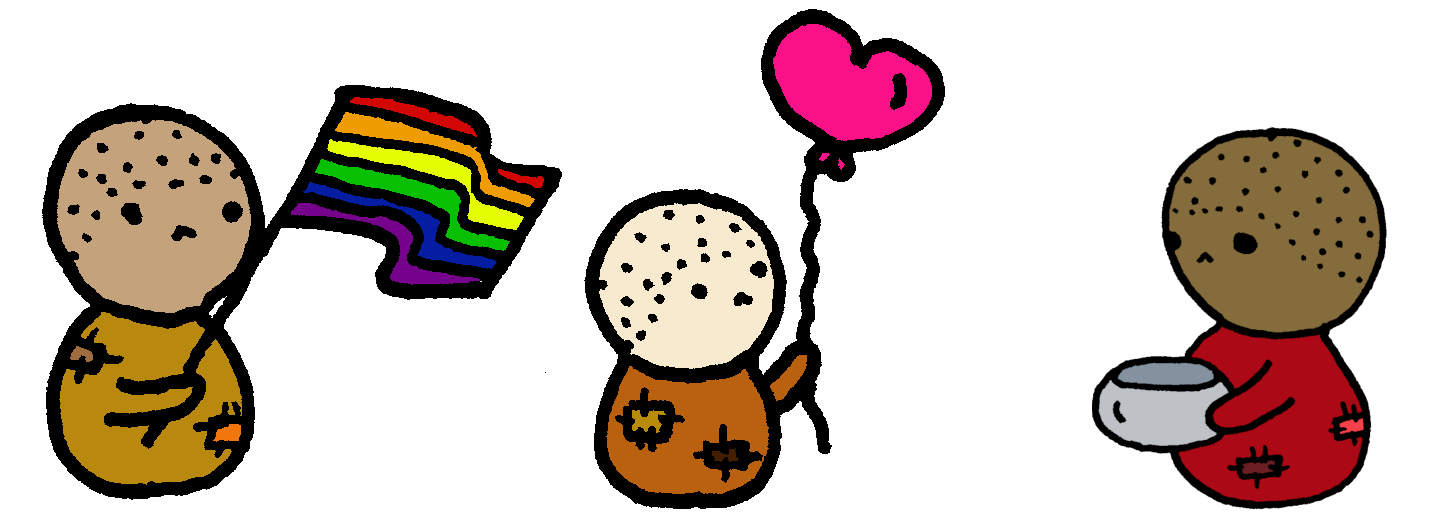
\includegraphics[width=0.8\paperwidth]{13.png}}
\end{figure}


\newpage
\thispagestyle{empty}
\begin{figure}[h]
    \centering
    \makebox[0pt]{%
    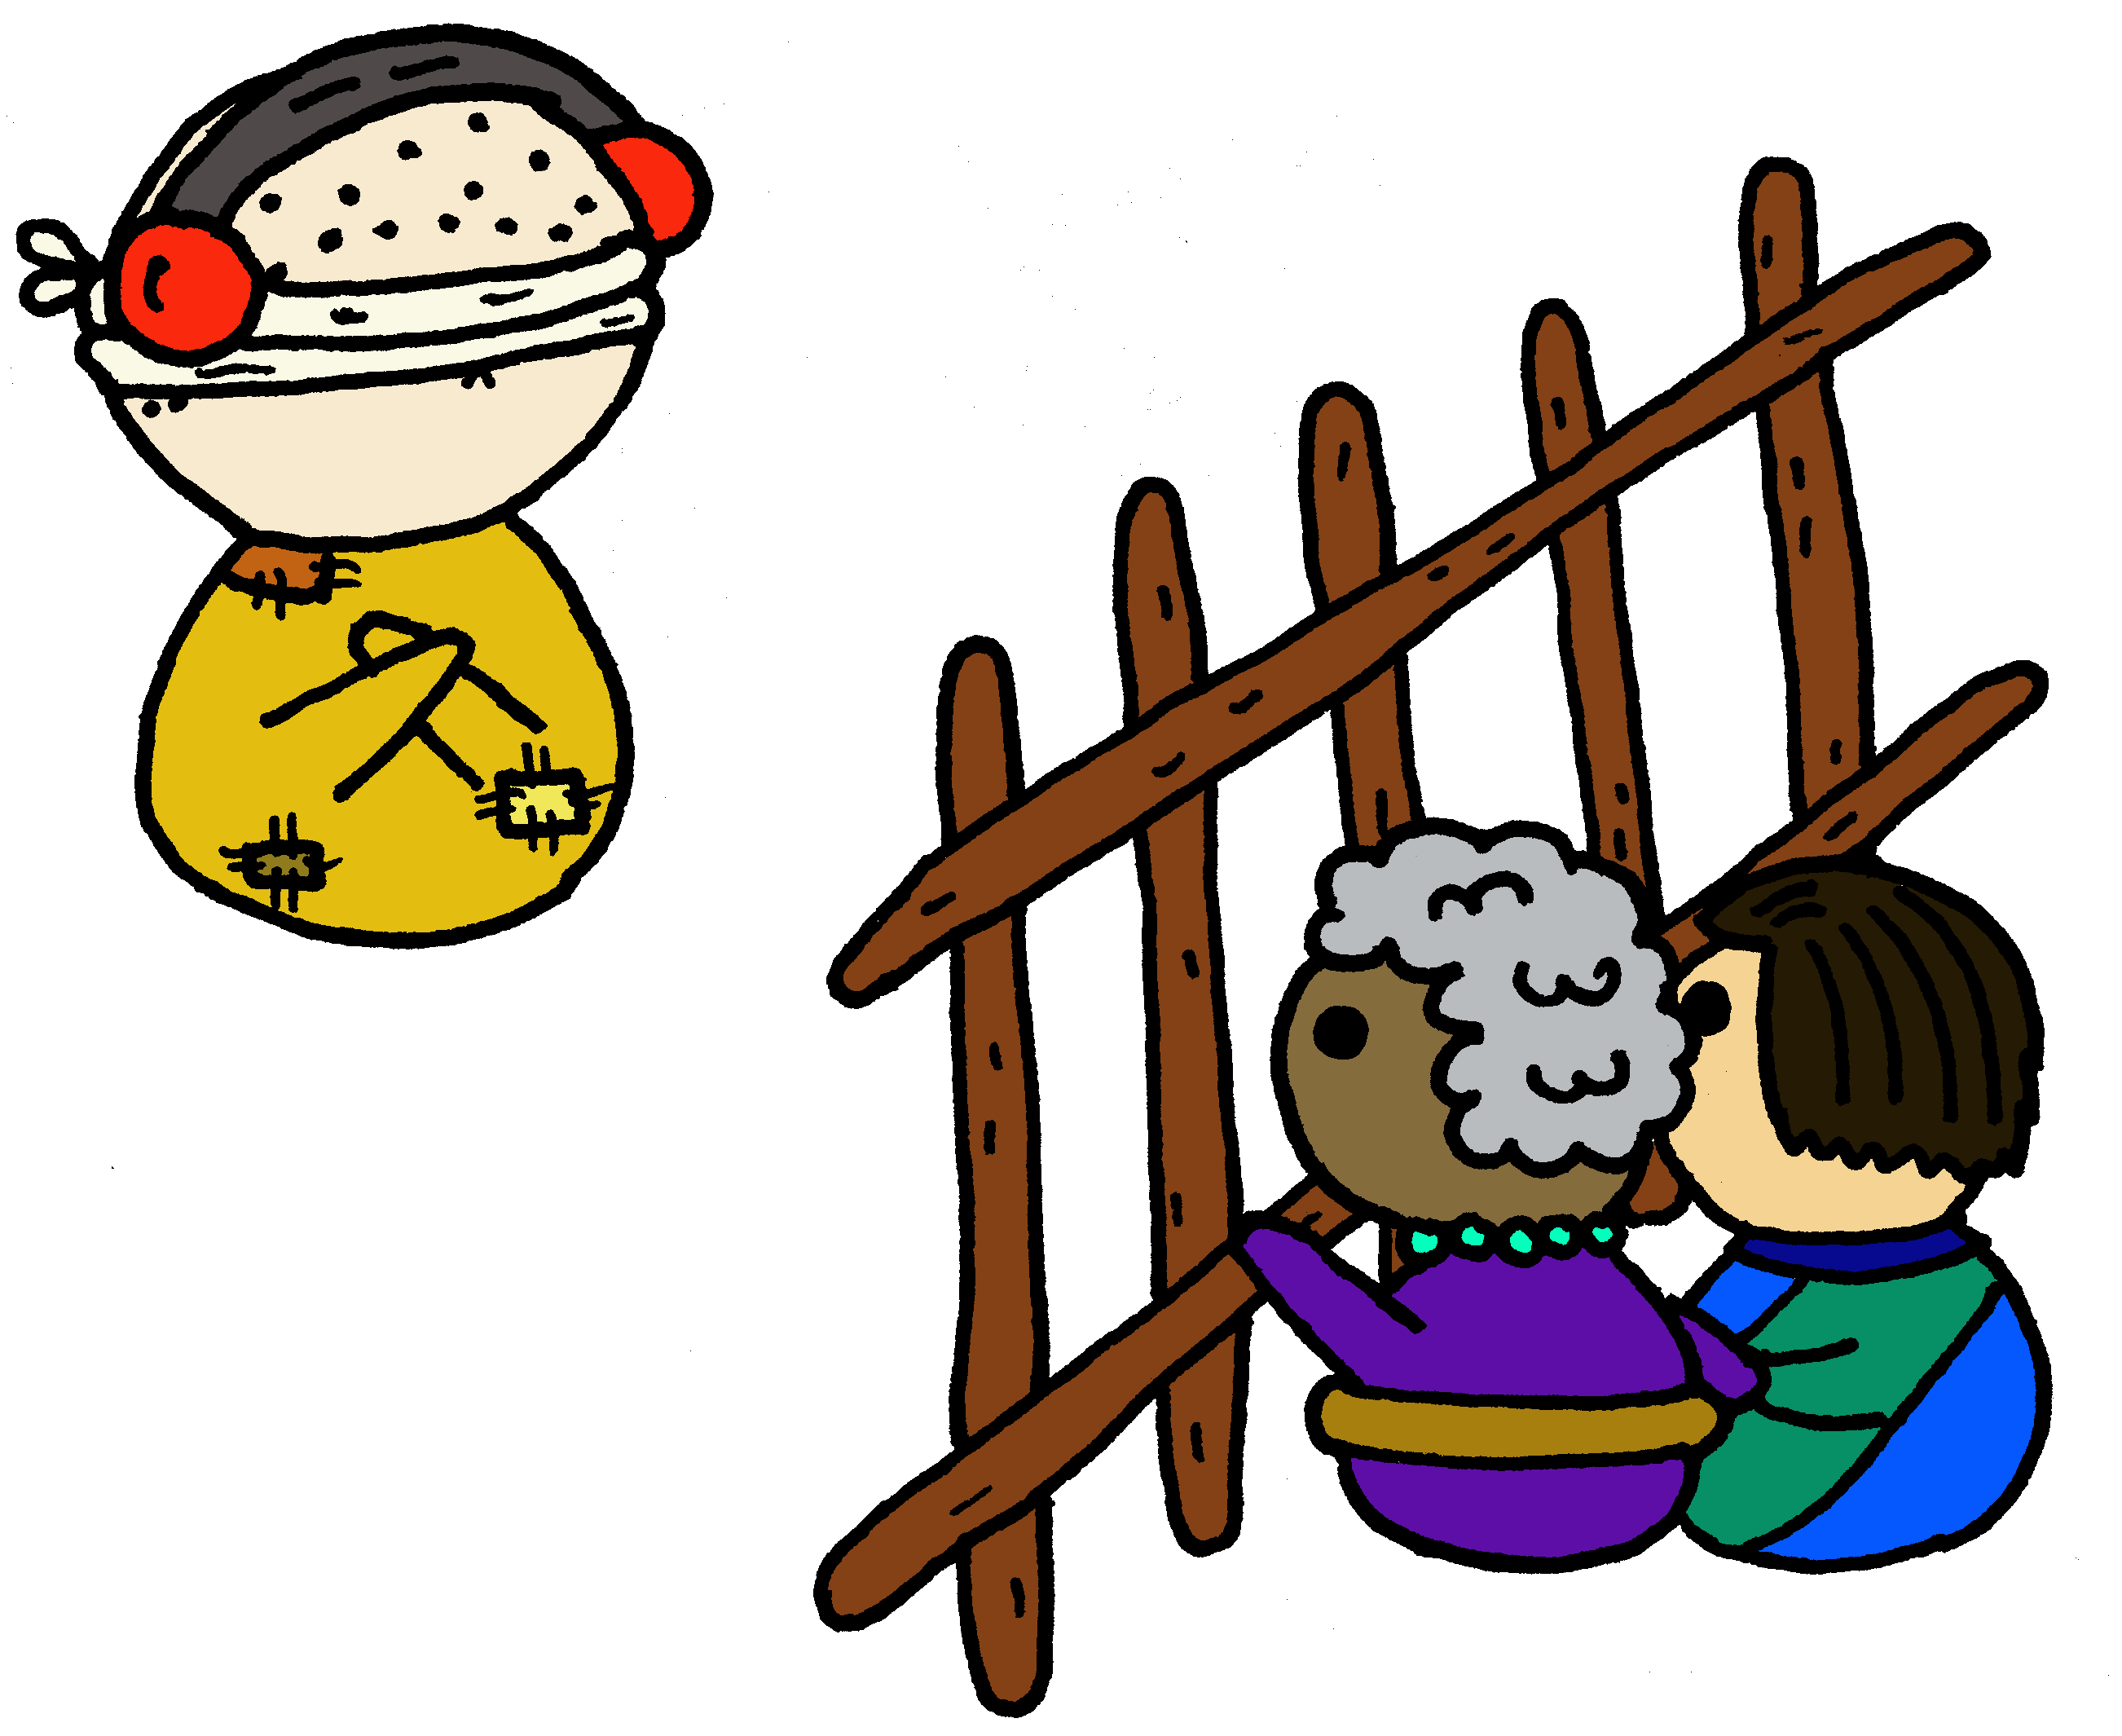
\includegraphics[width=0.8\paperwidth]{14.png}}
\end{figure}

\begin{quote}
\centering
\doublespacing
\textit{\Large \textcolor{blue}{\textbf{Si las personas y organizaciones budistas no son activamente inclusivas, las personas LGBTQIA+ seguirán siendo excluidas.}}}
\end{quote}

\chapter*{Obstáculos que impiden la inclusión de la personas LGBTQIA+}
\addcontentsline{toc}{chapter}{Obstáculos que impiden la inclusión de la personas LGBTQIA+}
\markboth{Darle la bienvenida al arcoíris}{Obstáculos que impiden la inclusión de la personas LGBTQIA+}

La forma en la que las organizaciones budistas se establecen y gestionan puede resultar en la posible exclusión de personas y de su participación. Por ejemplo, las barreras físicas, como los escalones, pueden excluir a las personas que usan sillas de ruedas; los edificios pueden tener rampas y ascensores para promover la inclusión. De igual manera, existen barreras administrativas, físicas y mentales que excluyen a las personas LGBTQIA+ de las cuales ni siquiera seamos conscientes, pero existen y tienen consecuencias tangibles.

\begin{quote}
\centering
\doublespacing
\textit{\Large \textcolor{blue}{\textbf{Podemos ayudar a eliminar todo aquello que excluye a las personas \mbox{LGBTQIA+} y así crear comunidades budistas más seguras e inclusivas.}}}
\end{quote}

\phantomsection
\section*{Obstáculos administrativos excluyentes}
\addcontentsline{toc}{section}{Obstáculos administrativos excluyentes}

Los formularios de registro, de membresía y las bases de datos en línea tienden a tener solamente opciones de hombre o mujer, lo cual excluye a muchas personas trans, personas no binarias y también a algunas personas intersexuales que prefieren no identificarse ni como hombre ni como mujer. Tener solo opciones binarias le muestra a estas personas que no son comprendidas ni bienvenidas, incluso antes de que se hayan inscrito en un retiro o se hayan unido a su boletín electrónico.

Para promover la inclusión, se puede añadir una opción alterna en los formularios que pregunten sobre el género, al igual que una opción como `X' además de las opciones de Sra. o Sr. El nombre y el género que algunas personas usan en la vida diaria pueden ser diferentes a lo que aparece en sus documentos de identificación oficiales, por lo que se pueden añadir opciones para preguntar por el nombre preferido y por los pronombres que usen les estudiantes. Considere también si es necesario incluir el género y el sexo en algunos formularios, o si esta información no tienen ningún fin concreto.

\phantomsection
\section*{Obstáculos físicos excluyentes}
\addcontentsline{toc}{section}{Obstáculos físicos excluyentes}

\subsubsection*{Asientos separados por género}

Algunos centros budistas tienen áreas de asientos diferenciados por género en sus salas de meditación, comedores y otros espacios. A veces, esto puede ser incluso un acomodo `jerárquico', con las mujeres sentadas detrás de los hombres. Las áreas públicas separadas por género no funcionan para todes en nuestra comunidad y pueden impedir que las personas se sientan seguras o que pertenezcan con les demás.

Para algunas personas trans, los espacios separados por género crean atención no deseada y miedo al rechazo. Para las personas no binarias, verse obligadas a tomar una decisión sobre dónde sentarse puede causar angustia cuando no se reconoce su género, mientras que a otras personas no les gusta la separación de género porque parece anticuada e innecesaria.

\subsubsection*{Baños}

\begin{wrapfigure}{r}{0.2\textwidth}
    \centering
    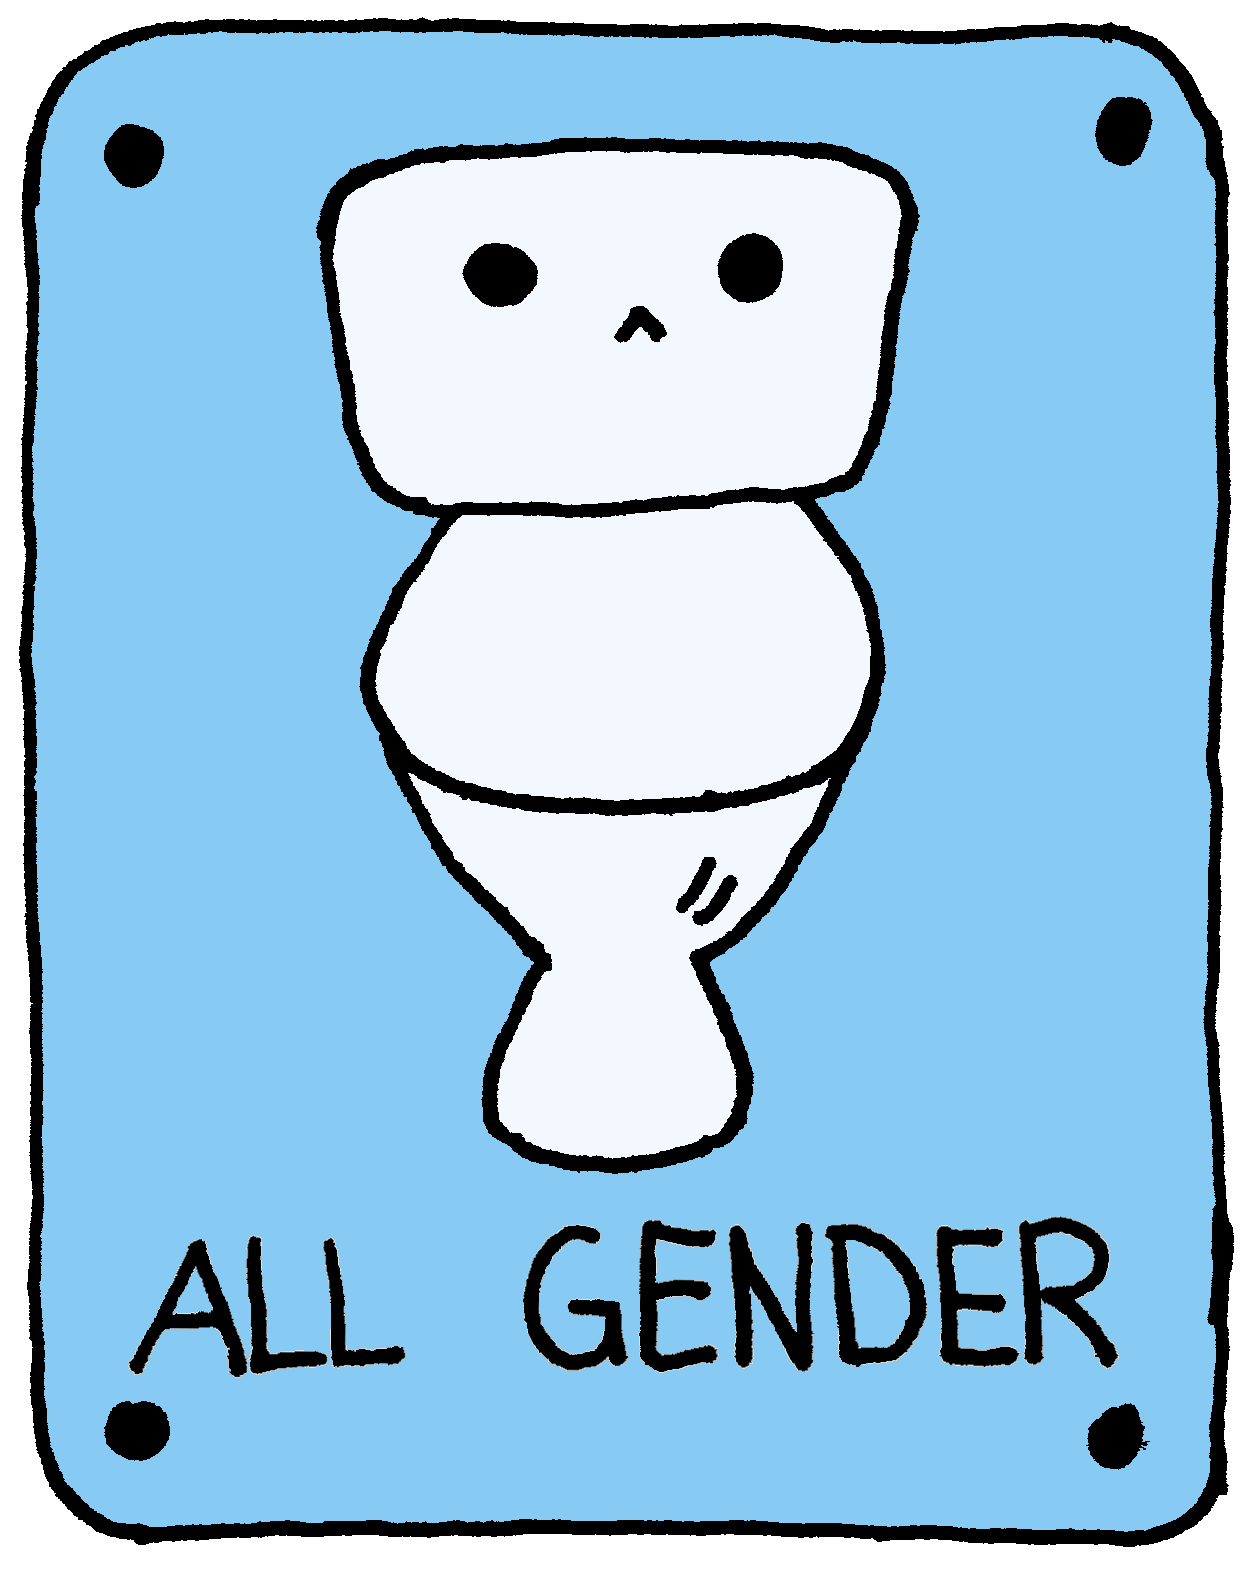
\includegraphics[width=0.2\textwidth]{16.png}
\end{wrapfigure}
Las personas deben sentirse cómodas para usar el baño que coincida con su identidad de género. Algunas personas trans y no binarias prefieren usar un baño neutro en lugar de tener que elegir entre baños para hombres y para mujeres. Asegurarse de que haya baños neutros en su centro y en los retiros ayuda a que las personas de género diverso se sientan seguras e incluidas.

\subsubsection*{Alojamiento durante los retiros}

Todes deben sentirse bienvenides y segures en un retiro, pero para muchas personas LGBTQIA+, los problemas de alojamiento pueden ser una razón de estrés. Pueden preocuparse por el rechazo debido a su sexualidad,  por ser excluidos por su género, o por sentir que sus necesidades simplemente no están siendo tomadas en consideración.

Todas las personas, ya sean cisgénero, trans o no binarias, deben tener derecho a elegir la opción de alojamiento que mejor se adapte a su identidad de género.
Ya que muchos centros de retiro dividen las instalaciones de alojamiento entre hombres y mujeres, es importante que las organizaciones sean conscientes de sus obligaciones jurídicas con respecto a la discriminación ilegal contra las personas trans que utilizan dichos espacios.

Siempre habrá una necesidad de alojamiento para un solo sexo, pero para ciertas personas trans y no binarias, dicha opción no reconoce que hay más identidades de género ni que hay personas que no se identifican ni como hombre ni como mujer. Las organizaciones de retiros pueden ofrecer diversas opciones de alojamiento para promover la inclusión y ofrecer alternativas seguras: una opción para mujeres, otra para hombres y otra para todos los géneros. Este tipo de opciones en los formularios le permiten a las personas escoger la opción que más prefieran.

Algunas personas que se sienten atraídas por personas su mismo género pueden preferir quedarse en un habitación neutra, ya que quedarse en una para un solo sexo puede ser una experiencia difícil: otras personas en su habitación podrían excluirles por ser homosexuales, o que el deseo se convierta en una distracción.

Por las razones anteriormente mencionadas, la opción de alojamiento neutro le permite a las personas trans, no binarias y a aquellas atraídas por su mismo sexo tomar una decisión oportuna. Otra opción podría ser la de ofrecer habitaciones privadas a las personas LGBTQIA+, haciendo que su experiencia de retiro será lo más cómoda posible.

He aquí algunos consejos para darle la bienvenida a la comunidad LGBTQIA+ en un retiro desde antes que empiece:

\begin{itemize}
  \setlength\itemsep{-0.3em}
  \item Asegúrate de que la publicidad indique que el retiro será un espacio seguro e inclusivo para personas LGBTQIA+
  \item Elabora formularios con opciones para diversos géneros, pronombres, y preferencias de alojamiento
  \item Asegúrate de que les voluntaries y gestores sean conscientes de prácticas inclusivas para personas LGBTQIA+
  \item Establece opciones de baños y alojamiento neutros usando señalización
  \item Recuérdale a les participantes durante la primera sesión que el retiro será un espacio seguro e inclusivo para todes, incluyendo a la comunidad LGBTQIA+.
\end{itemize}

\begin{figure}[h]
    \centering
    \makebox[0pt]{%
    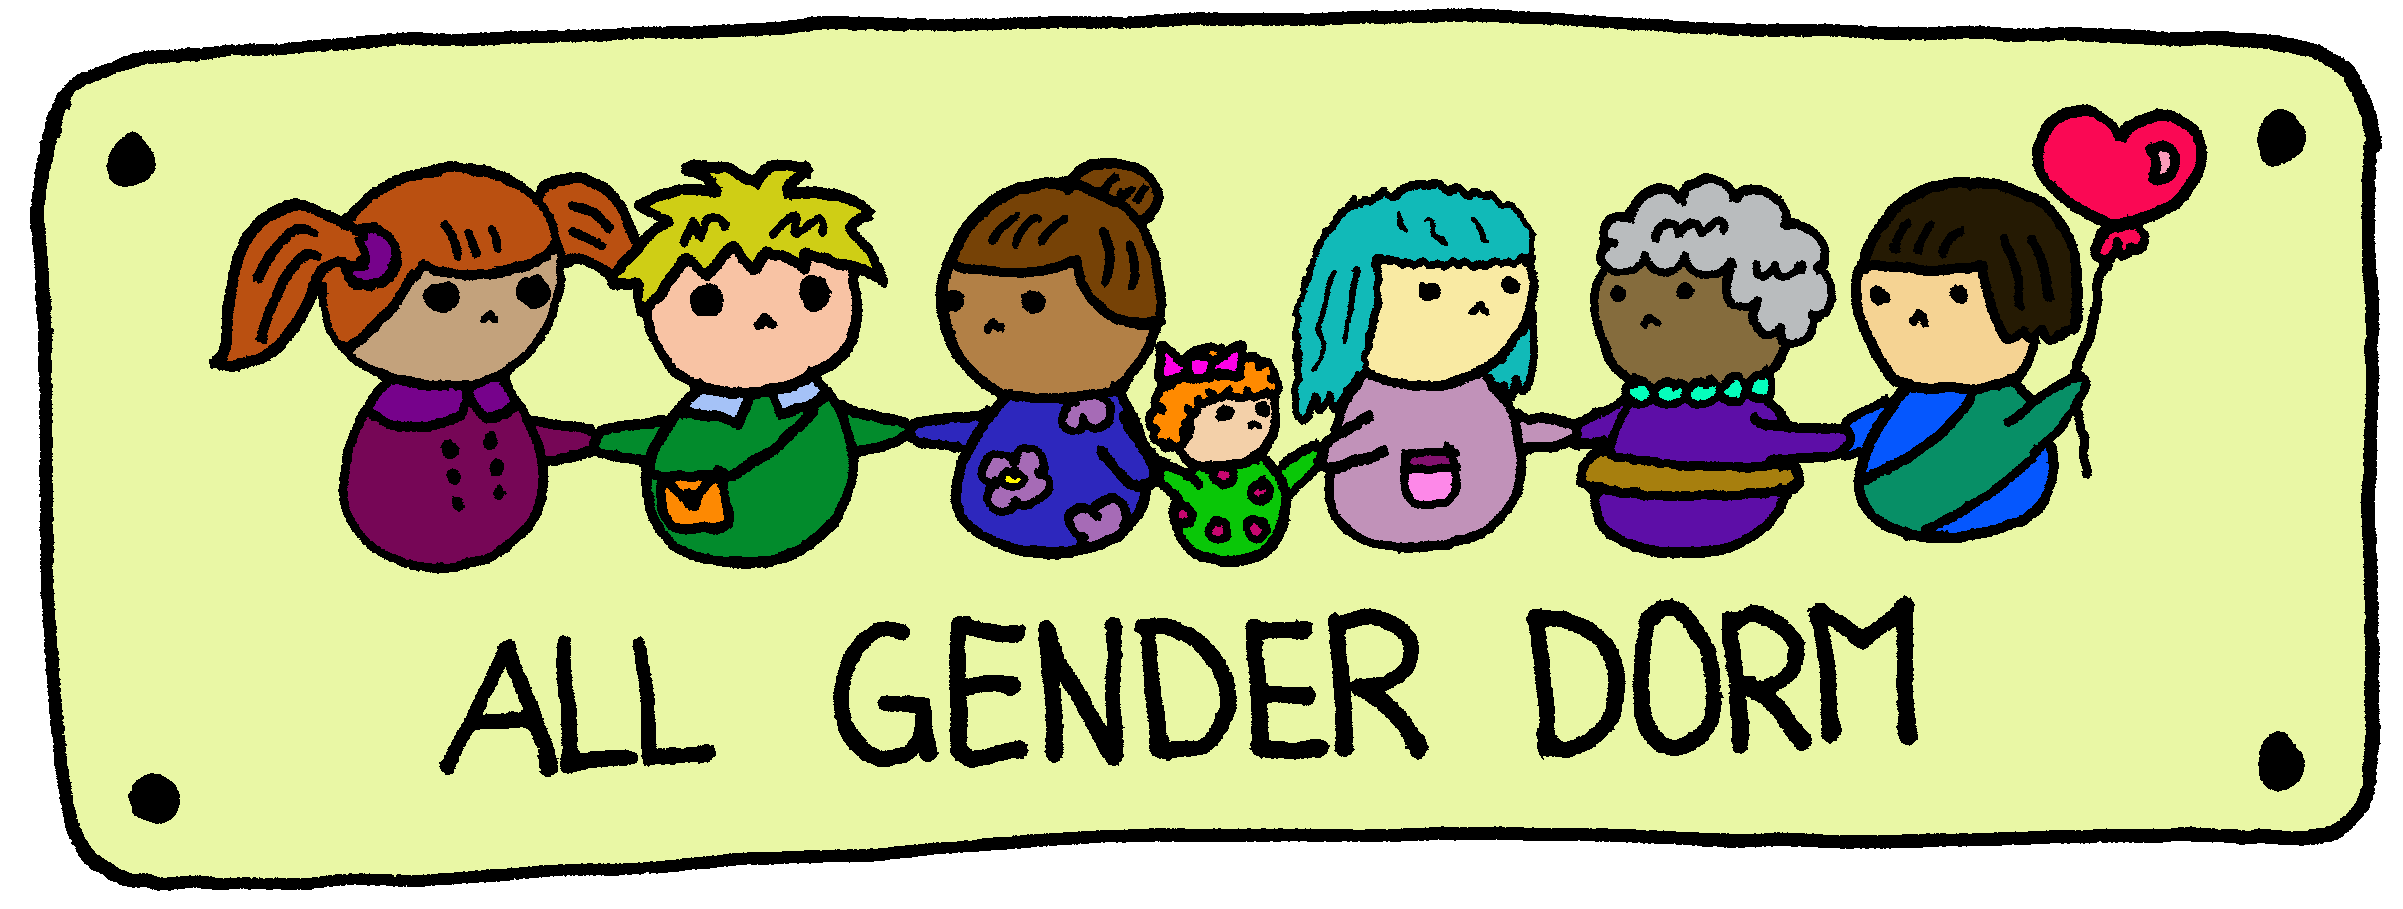
\includegraphics[width=0.6\paperwidth]{18-19.png}}
\end{figure}

\newpage
\thispagestyle{empty}
\begin{figure}[h]
    \centering
    \makebox[0pt]{%
    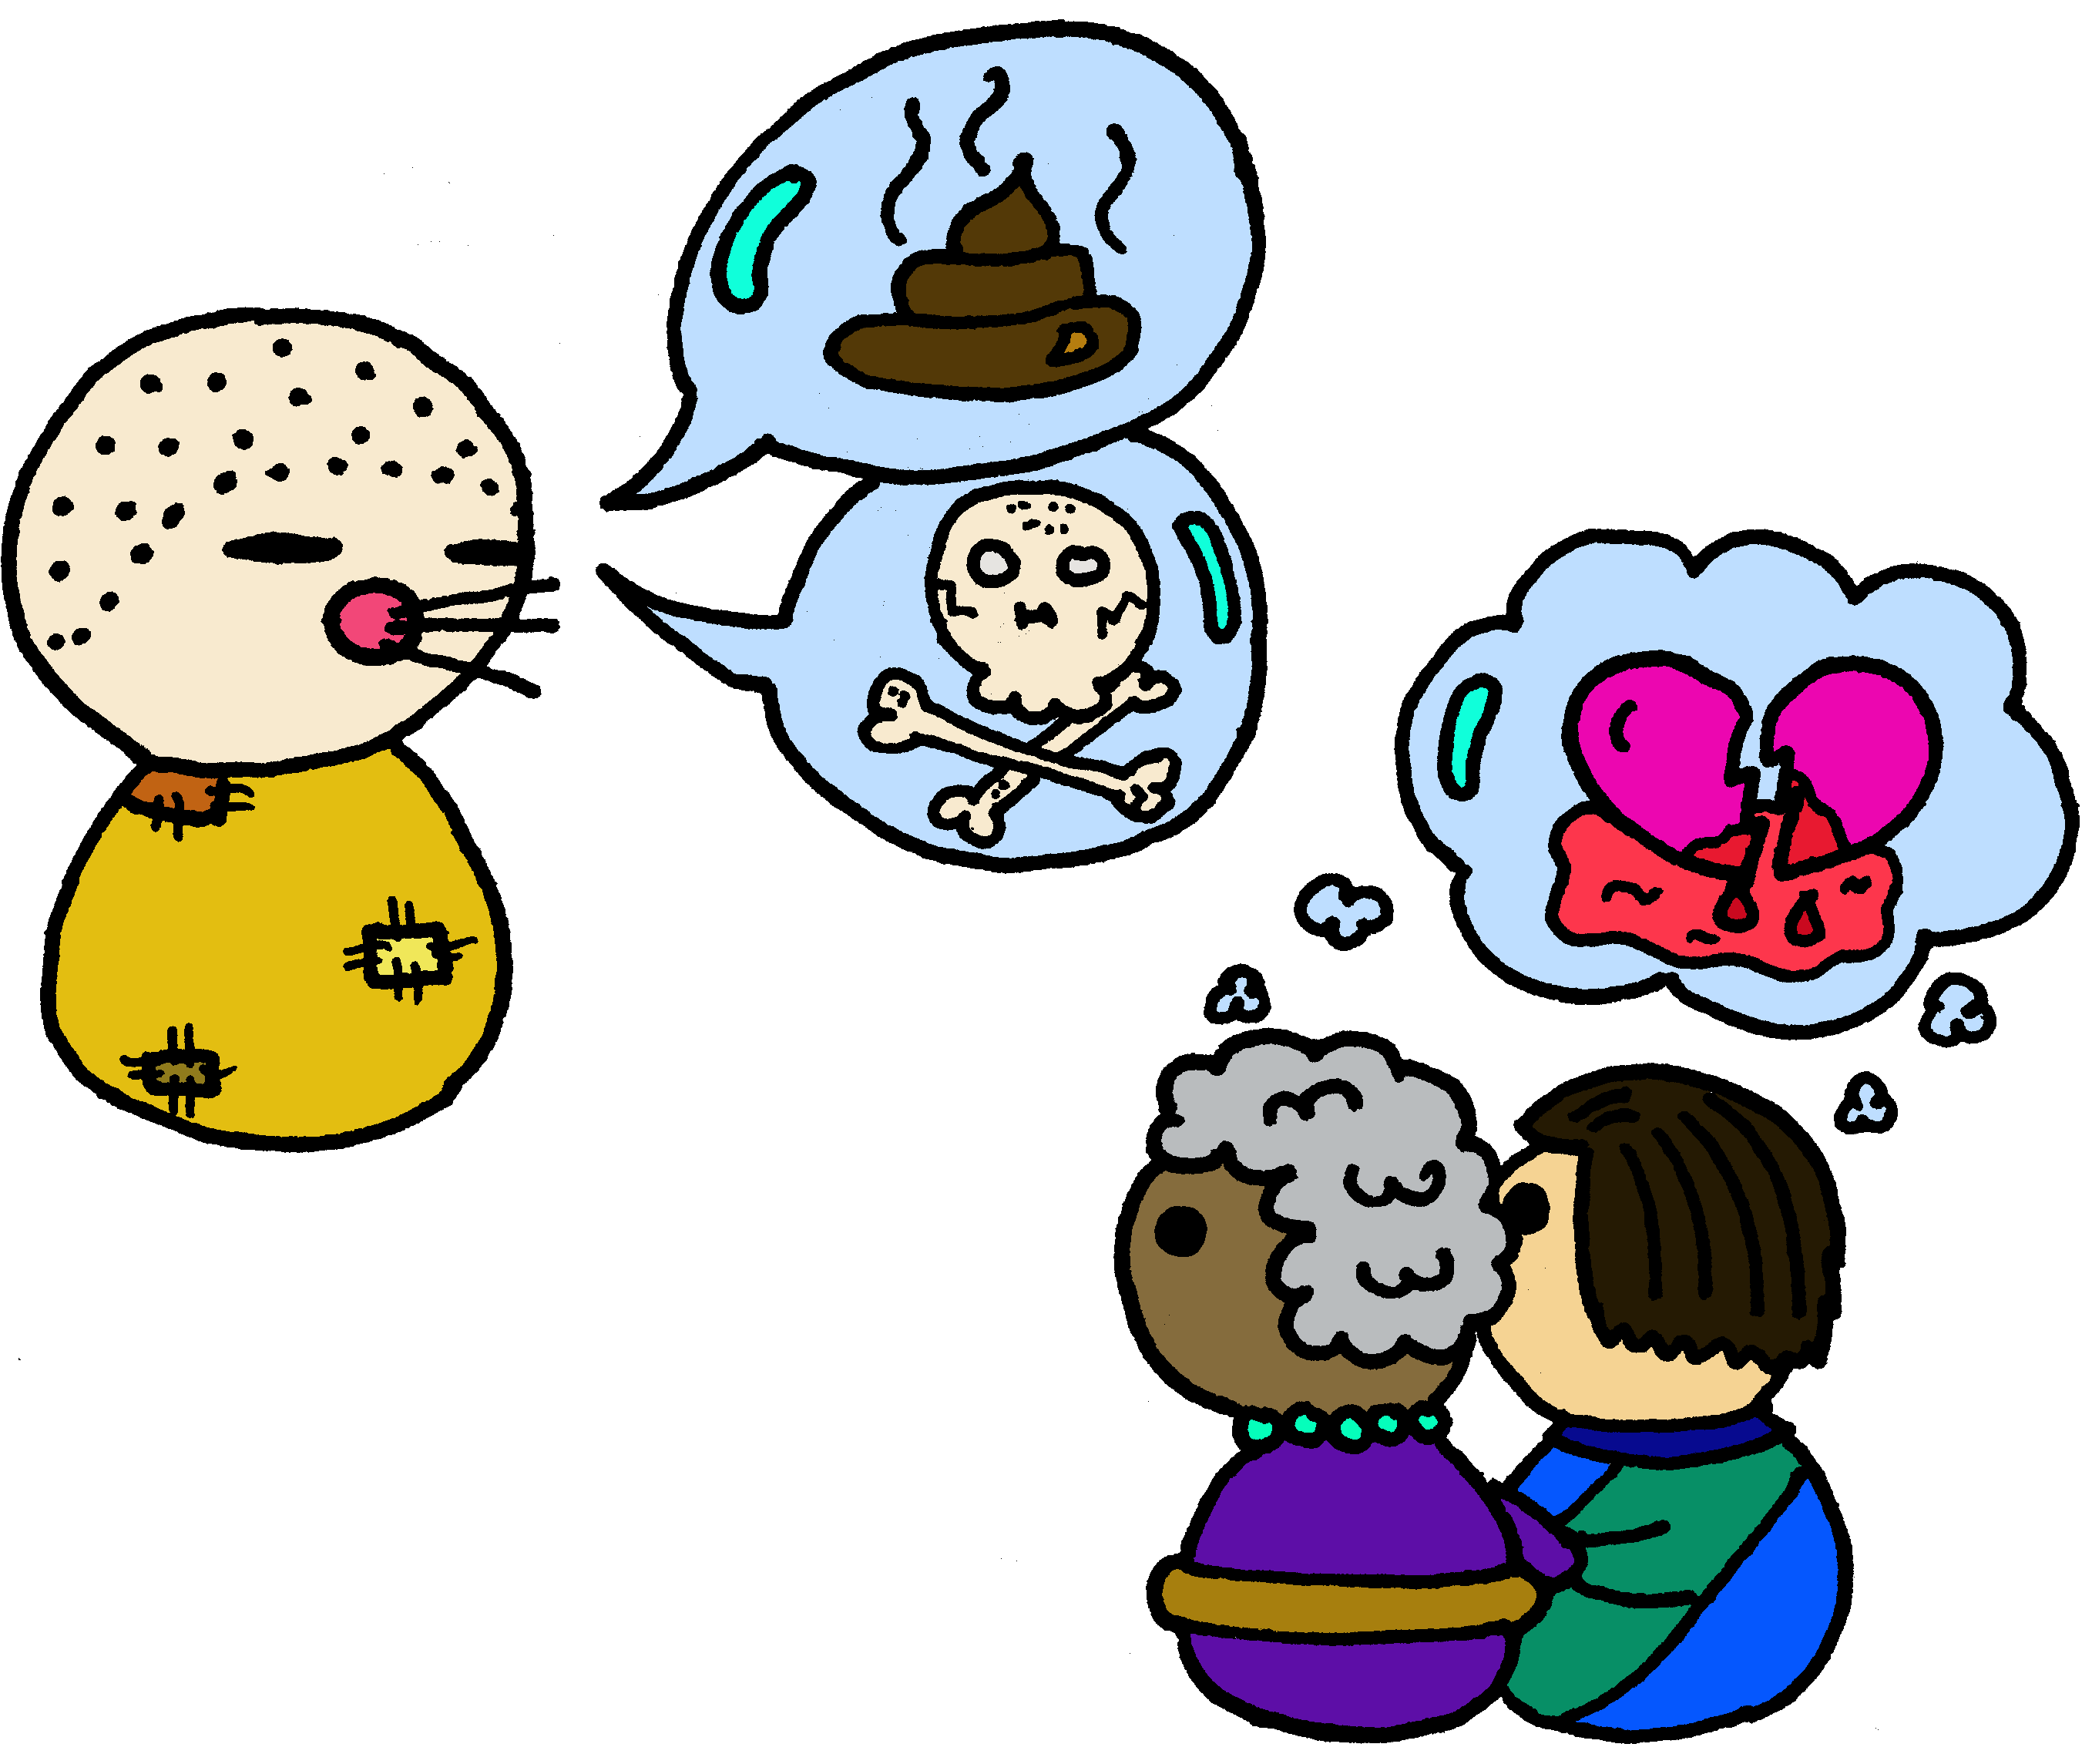
\includegraphics[width=0.8\paperwidth]{20.png}}
\end{figure}

\begin{quote}
\centering
\doublespacing
\textit{\Large \textcolor{violet}{\textbf{Nuestra habla puede otorgar seguridad, respeto e inclusión, pero también pueden causar incomodidad, daño y exclusión.}}}
\end{quote}

\chapter*{Lenguaje hiriente }
\addcontentsline{toc}{chapter}{Lenguaje hiriente }
\markboth{Darle la bienvenida al arcoíris}{Lenguaje hiriente }

\phantomsection
\section*{Palabras hirientes}
\addcontentsline{toc}{section}{Palabras hirientes}

El habla correcta es un concepto budista importante. Nuestras palabras tienen consecuencias: las palabras amables no dañan y muestran respeto por las personas de nuestra comunidad. Por otra parte, las palabras también pueden lastimar a las personas y hacer que no se sientan cómodes. El lenguaje irrespetuoso, los chistes ignorantes y las preguntas invasivas no son discursos correctos, y obstaculizan la participación de las personas LGBTQIA+ en las comunidades budistas.

Hay algunos elementos importantes que debemos tener en cuenta al hablar con personas LGBTQIA+.

\subsubsection*{Lenguaje irrespetuoso}

Sé amable siempre y sé consciente de las palabras que puedan lastimar; el discurso ofensivo puede tener también consecuencias legales.

\begin{itemize}
  \setlength\itemsep{-0.3em}
  \item Evita usar términos anticuados, como `hermafrodita', `transexual', y otras palabras parecidas; estas tienen connotaciones médicas que estigmatizan a las personas de la comunidad LGBTQIA+.
  \item No uses palabras peyorativas, como `marica', `puto', `lencha', `bollera', `tortillera', `trava', u otros términos despectivos que insulten a cualquier disidencia LGBTQIA+.
  \item Evita emplear oraciones que denigren a las personas LGBTQIA+, como `¡Qué gay!', o `eso es de maricones'.
\end{itemize}

\subsubsection*{Lenguaje excluyente}

Una buena forma de que nuestras comunidades budistas sean espacios seguros e inclusivos es ser conscientes de lo que decimos. He aquí algunos consejos al respecto:

\begin{itemize}
  \setlength\itemsep{-0.3em}
  \item Evita usar el lenguaje binario que excluye a las personas trans y no binarias. En lugar de decir `señoras y señores' o `hermanos y hermanas', puedes simplemente decir `hola a todes'.
  \item Evita usar lenguaje excluyente. En lugar de decir `la historia del hombre', puedes decir `la historia de la humanidad'. En lugar de decir `chicos' o `todos', di `todes'.
  \item Sé consciente de la exclusión en contra de personas que les atrae su mismo sexo. En lugar de decir `marido y mujer', puedes decir `pareja(s)'. En lugar de decir `atracción al  sexo opuesto', puede simplemente decir `atracción'.
  \item Nunca deshumanices a alguien enfocándote únicamente en su cuerpo o en su orientación sexual. Recuerda que todes somos personas holísticas y que somos más que solamente esos conceptos. No te refieras a alguien por su orientación sexual (`ese gay de allá') o por su historial médico (`es un hombre que se hizo mujer' o `todavía no se hace la cirugía').
\end{itemize}


\begin{figure}[h]
    \centering
    \makebox[0pt]{%
    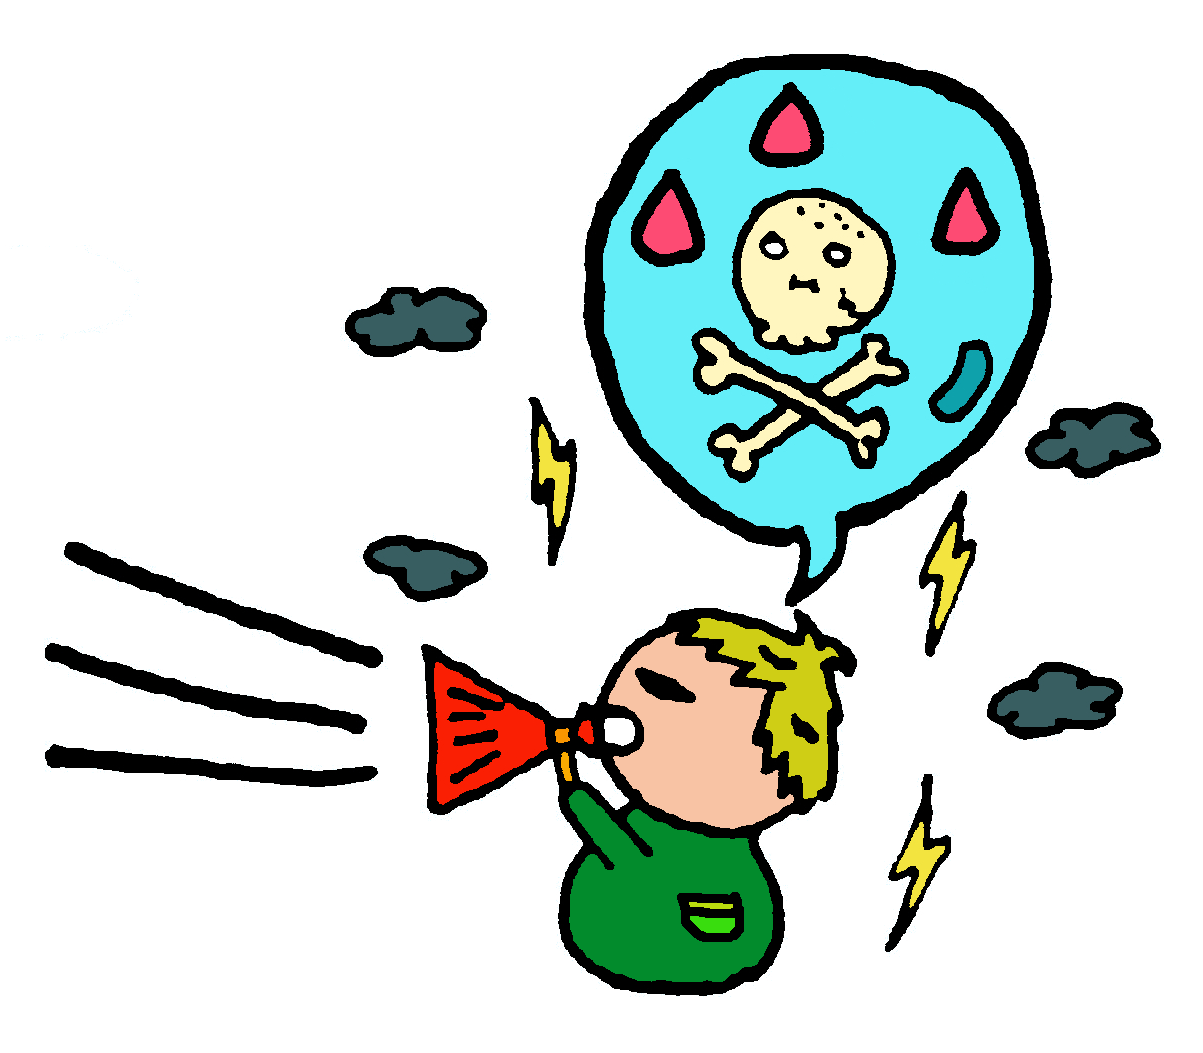
\includegraphics[width=0.6\paperwidth]{22.png}}
\end{figure}

\begin{quote}
\centering
\doublespacing
\textit{\Large \textcolor{violet}{\textbf{Todes se sienten bienvenides cuando usamos lenguaje inclusivo, mientras que muches son rechazades al usar lenguaje excluyente}}}
\end{quote}


\begin{figure}[h]
    \centering
    \makebox[0pt]{%
    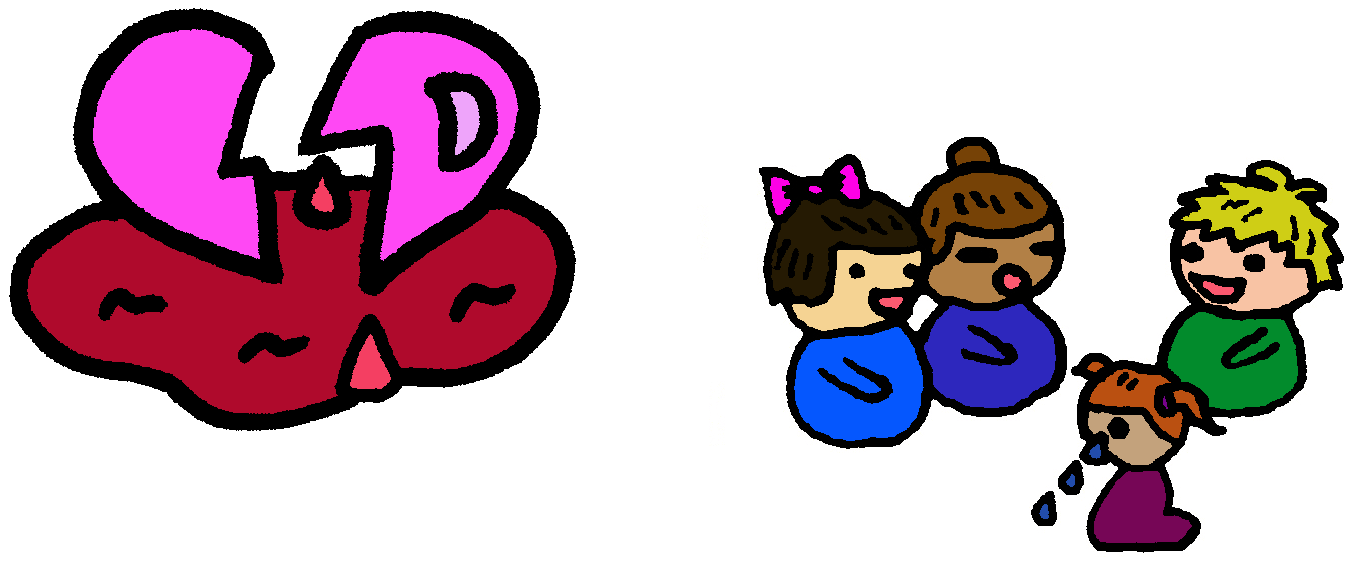
\includegraphics[width=0.6\paperwidth]{23.png}}
\end{figure}

\subsubsection*{Preguntas inapropiadas}

Las preguntas invasivas sobre la vida personal de les demás siempre serán inapropiadas en un espacio comunitario. El preguntarle a alguien sobre sus genitales, los procedimientos quirúrgicos que ha tenido, orientación o vida sexual es desagradable ya que todos estos elementos son parte de la vida privada de les demás. Algunas preguntas inapropiadas podrían ser:

\begin{itemize}
  \setlength\itemsep{-0.3em}
  \item ¿Eres hombre o mujer?
  \item ¿Te has hecho alguna cirugía?
  \item ¿Cuál era tu nombre antes de que hicieras la transición?
  \item ¿Quién es el hombre en la relación?
  \item ¿Cuál es tu rol sexual?
  \item ¿Alguna vez has tenido relaciones sexuales con alguien del sexo opuesto?
  \item Si eres bisexual, ¿cómo es que te casaste con una sola persona?
\end{itemize}

\subsubsection*{Insultos disfrazados de cumplidos}

Hacerle un cumplido a alguien por parecer heterosexual o cisgénero implica que es mejor que parecer LGBTQIA+, lo cual es ofensivo. Estos cumplidos tienen sus orígenes en estereotipos, mas no en el reconocimiento de la verdadera diversidad de nuestra comunidad.

\begin{figure}[h]
    \centering
    \makebox[0pt]{%
    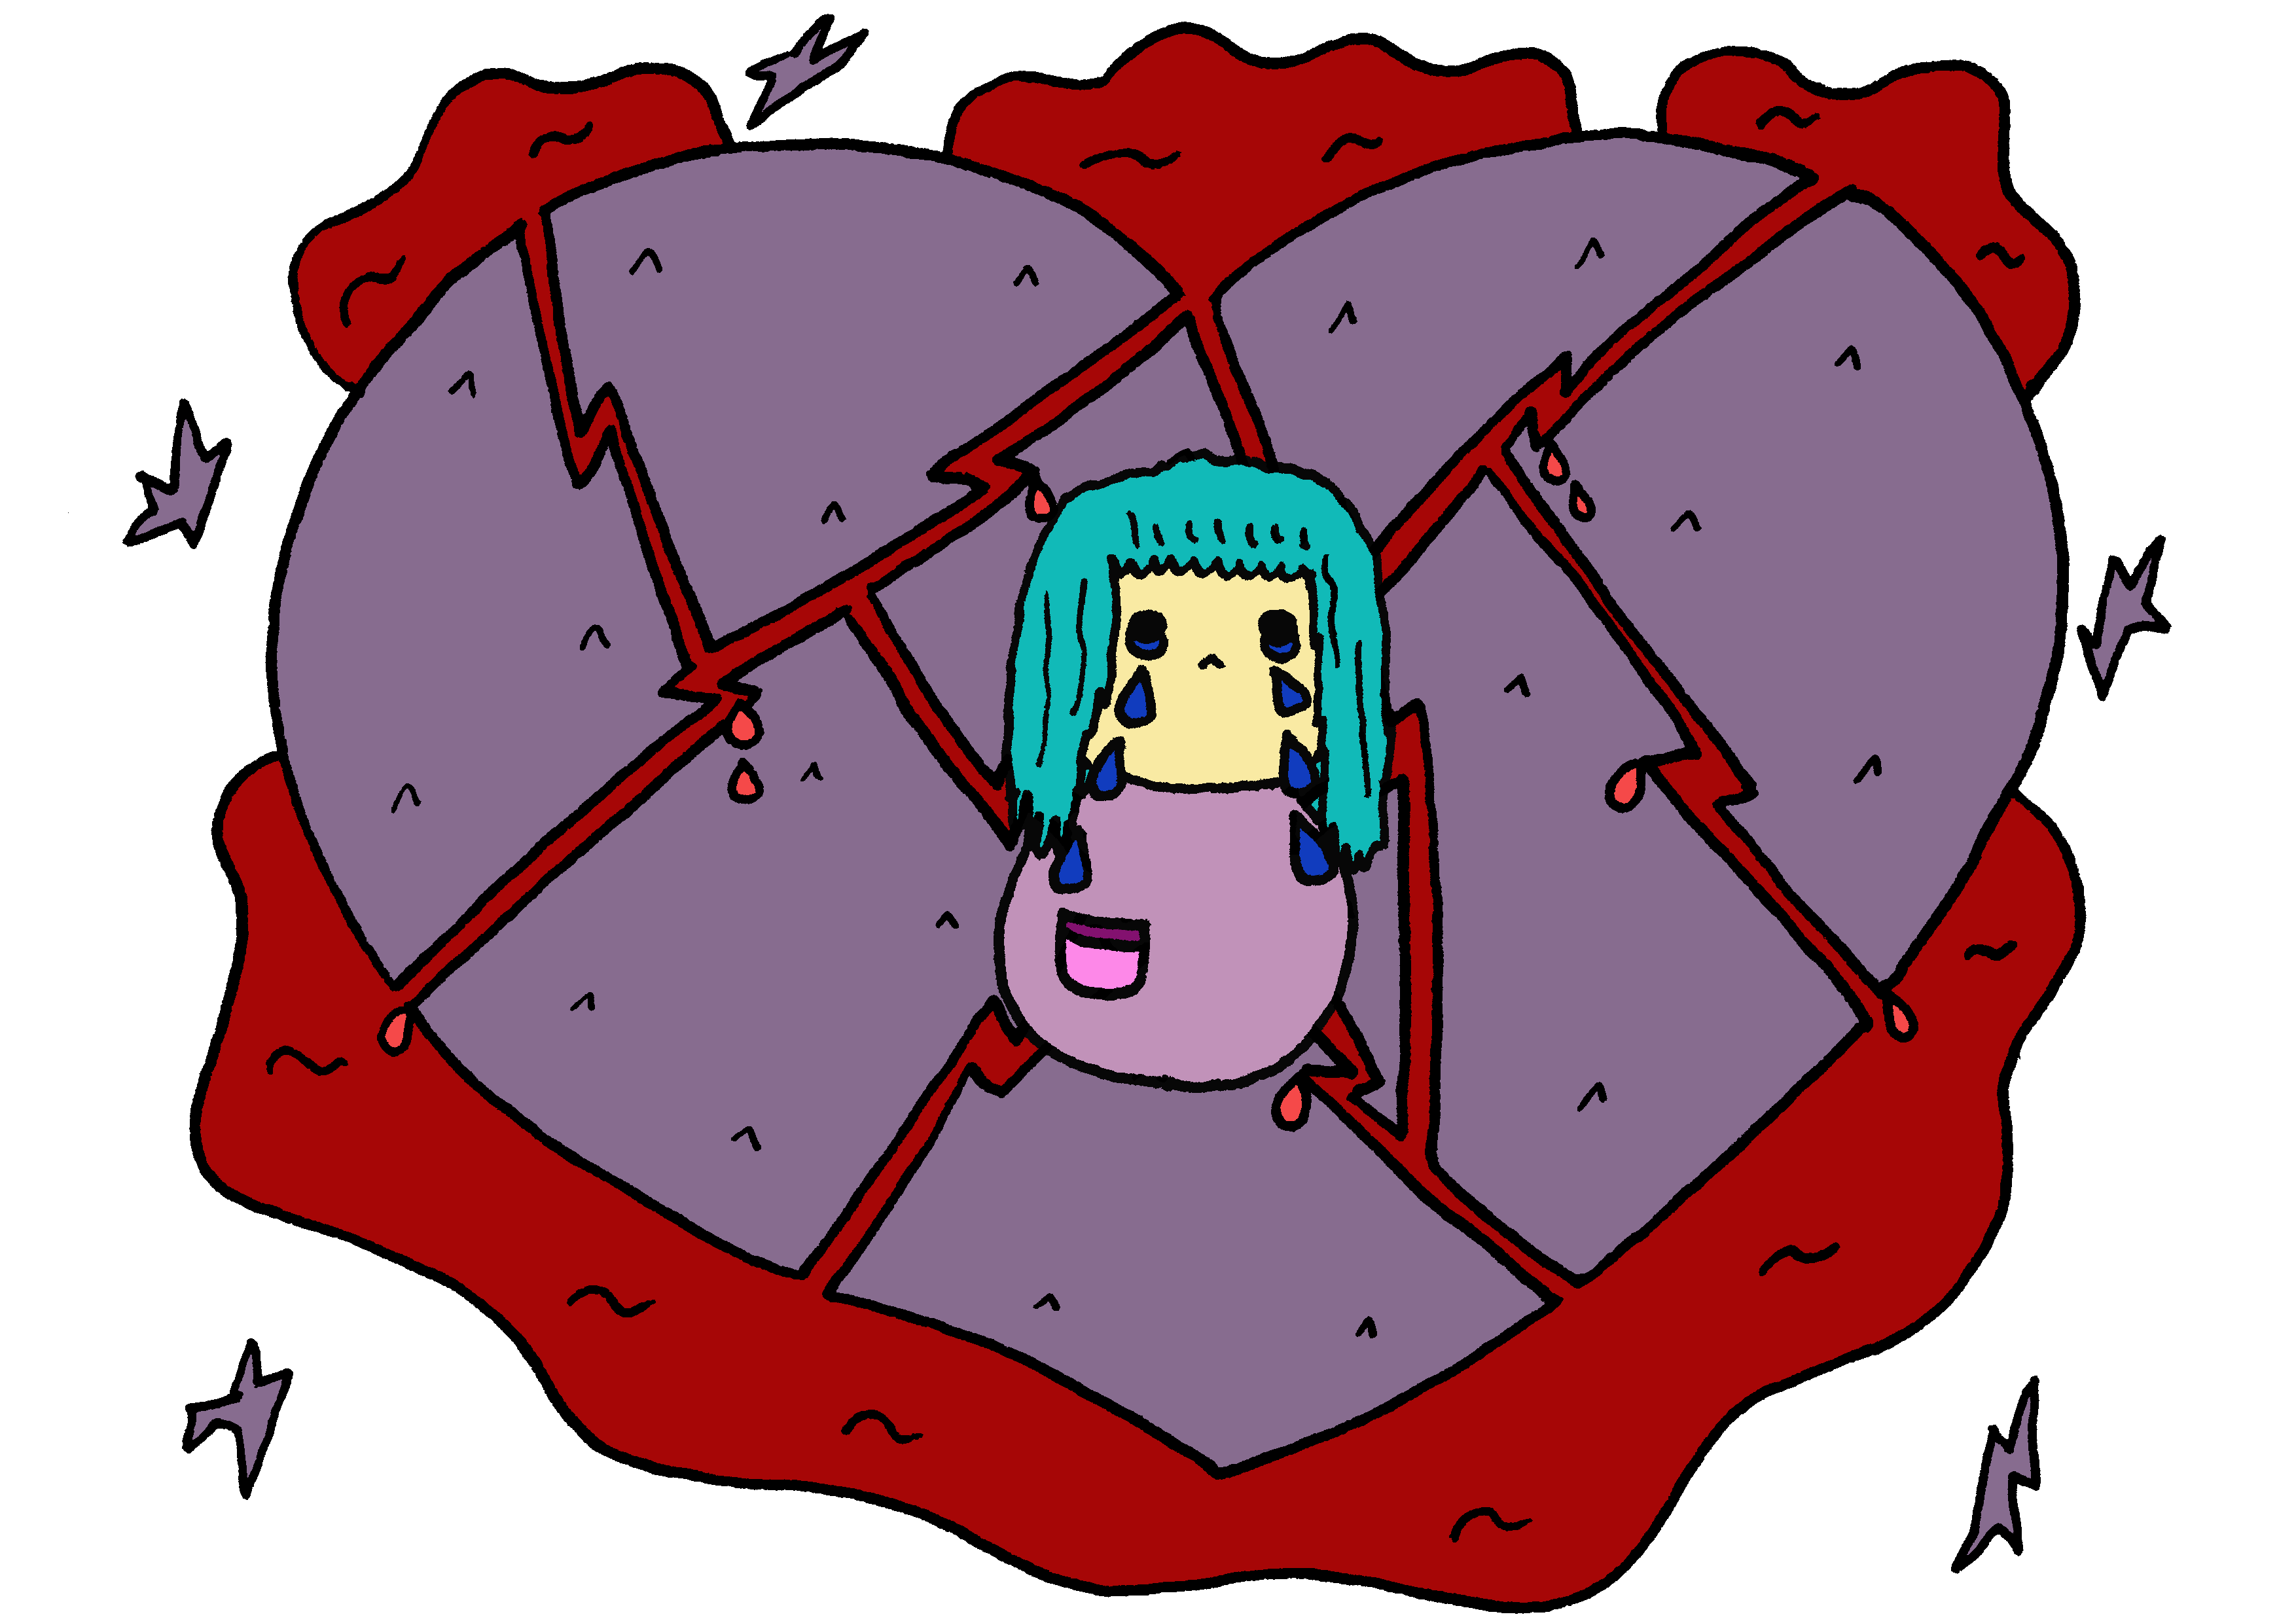
\includegraphics[width=0.35\paperwidth]{29.png}}
\end{figure}
\begin{itemize}
  \setlength\itemsep{-0.3em}
  \item `¡No pareces gay!'
  \item `Nunca hubiera imaginado que eres trans'
  \item `Para ser un hombre gay, eres bastante masculino'
  \item `No pareces lesbiana'
\end{itemize}

\subsubsection*{Bromas y chistes inapropiados}

Lo que para alguien puede ser gracioso puede también lastimar a alguien más. Generalmente, los chistes y bromas sobre el género, la sexualidad y los cuerpos de les demás no son graciosos, puesto que tienden a excluir, acosar o humillar. 

\subsubsection*{Bromas y chistes de doble sentido}

En un espacio de comunidad, siempre será inapropiado hacer gestos o comentarios sobre los cuerpos, el género o la sexualidad de les demás.

\subsubsection*{Estereotipos}

Al caer en estereotipos, negamos la individualidad de las personas a las cuales nos referimos. Recuerda que hay muchas diferencias entre los grupos de la comunidad LGBTQIA+; no todes tienen los mismos gustos o intereses.

\subsubsection*{Sacar del armario a alguien (Outing)}

No expongas la sexualidad o el género de alguien más sin su permiso. Chismorrear sobre estos temas lastima a otras personas y es además habla incorrecta.

\begin{figure}[h]
    \centering
    \makebox[0pt]{%
    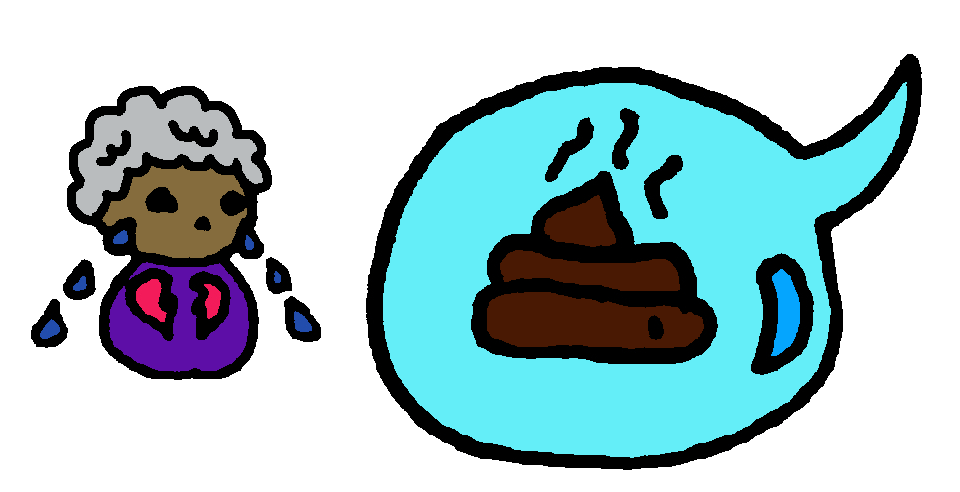
\includegraphics[width=0.45\paperwidth]{24.png}}
\end{figure}

\phantomsection
\section*{La importancia de los pronombres}
\addcontentsline{toc}{section}{La importancia de los pronombres}

A todes nos gusta que se reconozca y respete nuestras identidades.

Los pronombres son palabras que se emplean para referirse a las personas sin tener que mencionar su nombre, como `yo' o `tú', y pueden también describir el género, como es el caso con `él' o `ella'. Tal y como las personas cisgénero, las personas trans o de género diverso también quieren que se refieran a ellas con los pronombres correctos. Los pronombres son, junto con los nombres, parte de la identidad de las personas.

\begin{figure}[h]
    \centering
    \makebox[0pt]{%
    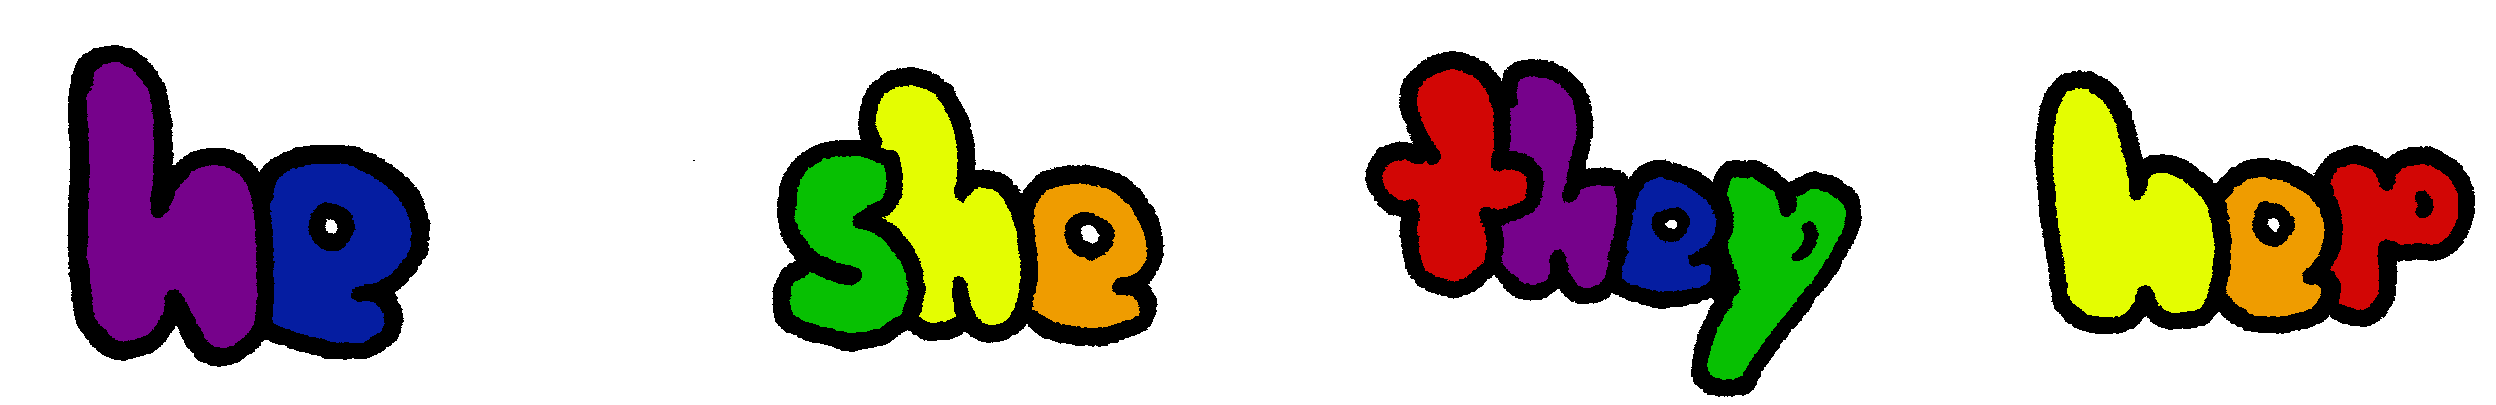
\includegraphics[width=0.7\paperwidth]{26.png}}
\end{figure}

Generalmente, el pronombre de alguien hace referencia a su identidad de género. Sin embargo, el género es un espectro: cómo alguien se ve o suena no implica que así se identifique. Por ello, no debemos asumir los pronombres de alguien meramente por su apariencia o su forma de hablar. Debemos, pues, preguntarles de manera discreta cuáles son sus pronombres para así emplearlos cuando estemos en su cercanía o con otras personas.

\noindent\fbox{%
    \parbox{\textwidth}{%
\textit{\textbf{\Large \textcolor{white}{El pronombre `elle' y el masculino genérico}}}

\bigskip

\textcolor{white}{El pronombre `elle' se usa para referirse, generalmente, a personas cuyas identidades van más allá de las opciones `hombre' o `mujer'. Un ejemplo de su uso es: `Elle me dio su paraguas antes de irse'. En español, tendemos a usar la `o' del masculino genérico para referirnos o adjetivar a un grupo de personas sin importar cómo se identifican, siempre y cuando haya un solo hombre en dicho grupo. Para evitar este masculino genérico que puede invisibilizar a otras personas que no se identifican como hombres, podemos recurrir a usar la `e' en el discurso oral y la `e' y/o la `x' en discursos escritos: `todes', `todxs', `les demás', `lxs demás', `sabies', `sabixs'…}
    }%
}

\subsubsection*{Tipos de pronombres}

Los pronombres tradicionales son `él', `ella', `ellos' y `ellas', pero hay ciertas personas que se identifican más allá del binarismo hombre/mujer y deciden usar otros pronombres, como `elle'. Otras prefieren usar `él' y `ella' para demostrar que su género es fluído, y otras más preferirán que se refieran a ellas únicamente con nombre de pila.

\subsubsection*{Emplea los pronombres correctos}

Para demostrar la importancia de los pronombres, podemos emplear el lenguaje inclusivo en nuestros centros budistas, lo cual ayudará a que las personas trans y de género diverso se sientan bienvenides, comprendides e incluídes.

\begin{itemize}
\setlength\itemsep{-0.3em}
\item Preséntate mencionando tus pronombres. Por ejemplo: `Hola, me llamo Bodhi y mi pronombre es ‘ella’'.
\item Si es apropiado, pregunta de forma discreta y amable para saber qué pronombres usa alguien más: `Hola, me llamo Pema y mi pronombre es ‘elle’. ¿Cómo quieres que me refiera a ti?'
\item Emplea siempre los pronombres y el nombre que la persona use en ese momento, incluso cuando te refieras a esa persona hablando de su pasado.
\item Si alguien malgeneriza o usa un nombre incorrecto al referirse a alguien más, hazles notar ese error y ayúdales a entender la importancia del uso del nombre y pronombre correctos.
\item Añade tus pronombres al final de tus correos electrónicos, perfiles digitales o en tu biografía. Por ejemplo: `Mitra Lovegood (ella), contadora'.
\end{itemize}\begin{figure}[h]
    \centering
    \makebox[0pt]{%
    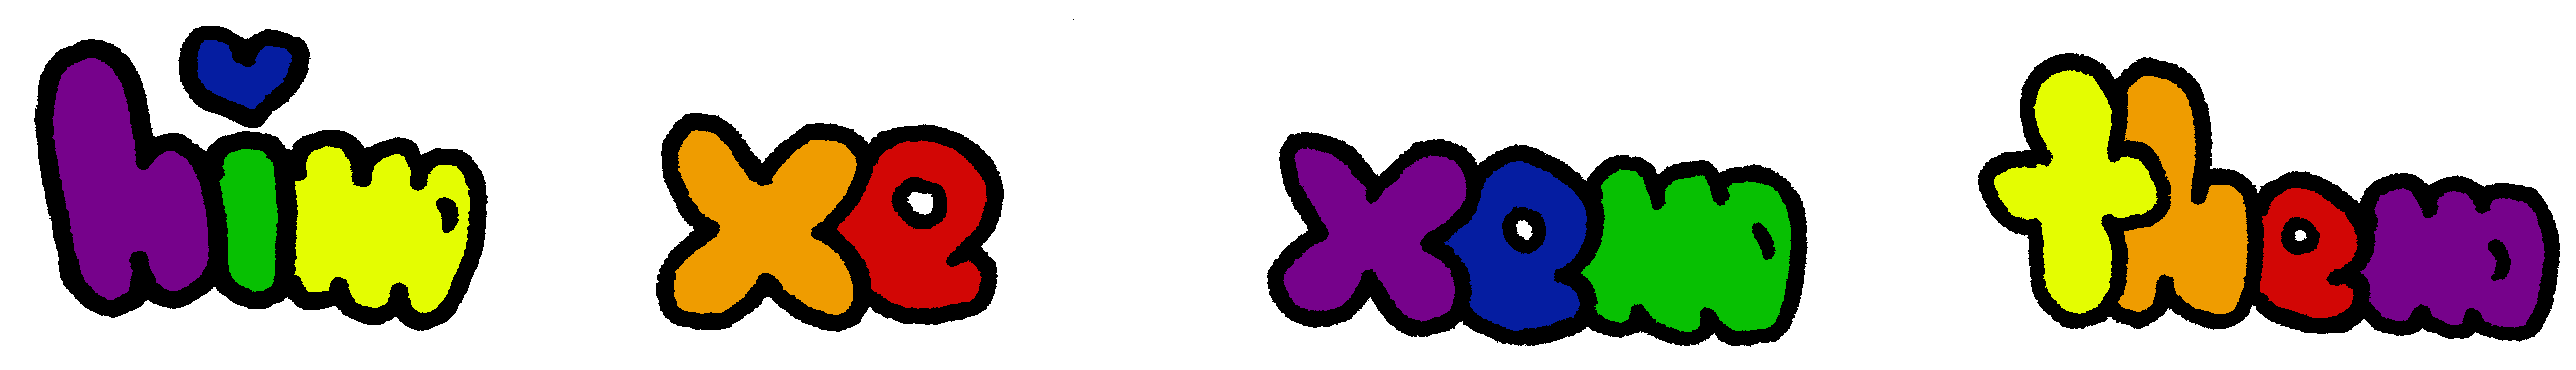
\includegraphics[width=0.7\paperwidth]{27.png}}
\end{figure}

Toma en consideración que habrán ciertas personas que no van a querer mencionar sus pronombres, y no se debe forzar a nadie a que los mencione.

\phantomsection
\section*{Malgenerizar (cometer misgendering)}
\addcontentsline{toc}{section}{Malgenerizar (cometer misgendering)}

La acción de malgenerizar sucede cuando describimos o nos referimos a alguien usando palabras que no van de acuerdo a cómo se identifica esa persona. El referirnos a alguien como desee que sea nombrada es un acto de amabilidad elemental. Cuando malgenerizamos, les demás se sentirán invalidades, ignorades y lastimades, y no se sentirán incluides. Una forma sencilla de respetar la identidad de género de una persona es preguntarle por sus pronombres, y usarlos correctamente. Si no sabes los pronombres de alguien, puedes optar por usar el Lenguaje No binario Indirecto (LNI), en el que intentas eliminar cualquier marca de género explícita. Por ejemplo, en vez de decir `ella es una estudiante', puedes decir `es parte del alumnado'. Una vez que conozcas los pronombres de alguien, úsalos correctamente. Si hay una persona que se identifica como hombre o mujer y así te lo indica, no uses pronombres neutros o LNI: usa los pronombres que esa persona te indique.

¡Está bien si te equivocas! Todes lo hacemos de vez en cuando, así que si usas un pronombre incorrecto, pide perdón, usa el pronombre correcto y no hagas un drama. Si te diste cuenta de un error después de una conversación, pide disculpas de forma privada y sigue con tu vida.

\subsubsection*{Uso del necrónimo (Deadnaming o Misnaming)}

Los nombres son importantes para todes, y usar el nombre correcto de alguien es un acto de amabilidad básico. El necrónimo es el nombre de una persona antes de que realizara su transición. Si nos referimos a una persona trans con su necrónimo, la vamos a lastimar. Nunca le pidas a alguien que te diga el nombre que tenía antes de su transición y cuando alguien haya decidido reafirmar su identidad con un nuevo nombre, debes emplear dicho nuevo nombre para mostrar tu apoyo y respeto.

\phantomsection
\section*{Instrucciones incómodas}
\addcontentsline{toc}{section}{Instrucciones incómodas}

Les maestres de meditación tienen que ser conscientes de que hay ciertas personas trans que se sienten incómodes con sus cuerpos. El sentimiento de angustia que surge por la incongruencia entre el sexo asignado al nacer y la identidad de género es conocido como `disforia de género'. Si une meditadore lidia con este problema, propón técnicas meditativas que no se centren en áreas del cuerpo que gatillen dicha disforia. Si, por ejemplo, une meditadore lidia con disforia de género sobre su pecho, propón una meditación en el caminar o una meditación sobre el amor bondadoso o cualquier otra técnica que no se enfoque en el área del pecho.

Cuando estamos en un grupo, es buena idea plantear distintas técnicas meditativas. Esto puede ser sumamente útil si hay personas novatas en la meditación y todavía no tienen las herramientas necesarias para controlar sus emociones o sensaciones desagradables.

Les maestres deben también tomar en cuenta el uso de lenguaje que incluye a todes sin importar el cuerpo, identidad de género, orientación sexual, y no deben asumir que todes les estudiantes son heterosexuales y/o cisgénero.

\newpage
\thispagestyle{empty}

\vfill

\begin{figure}[h]
    \centering
    \makebox[0pt]{%
    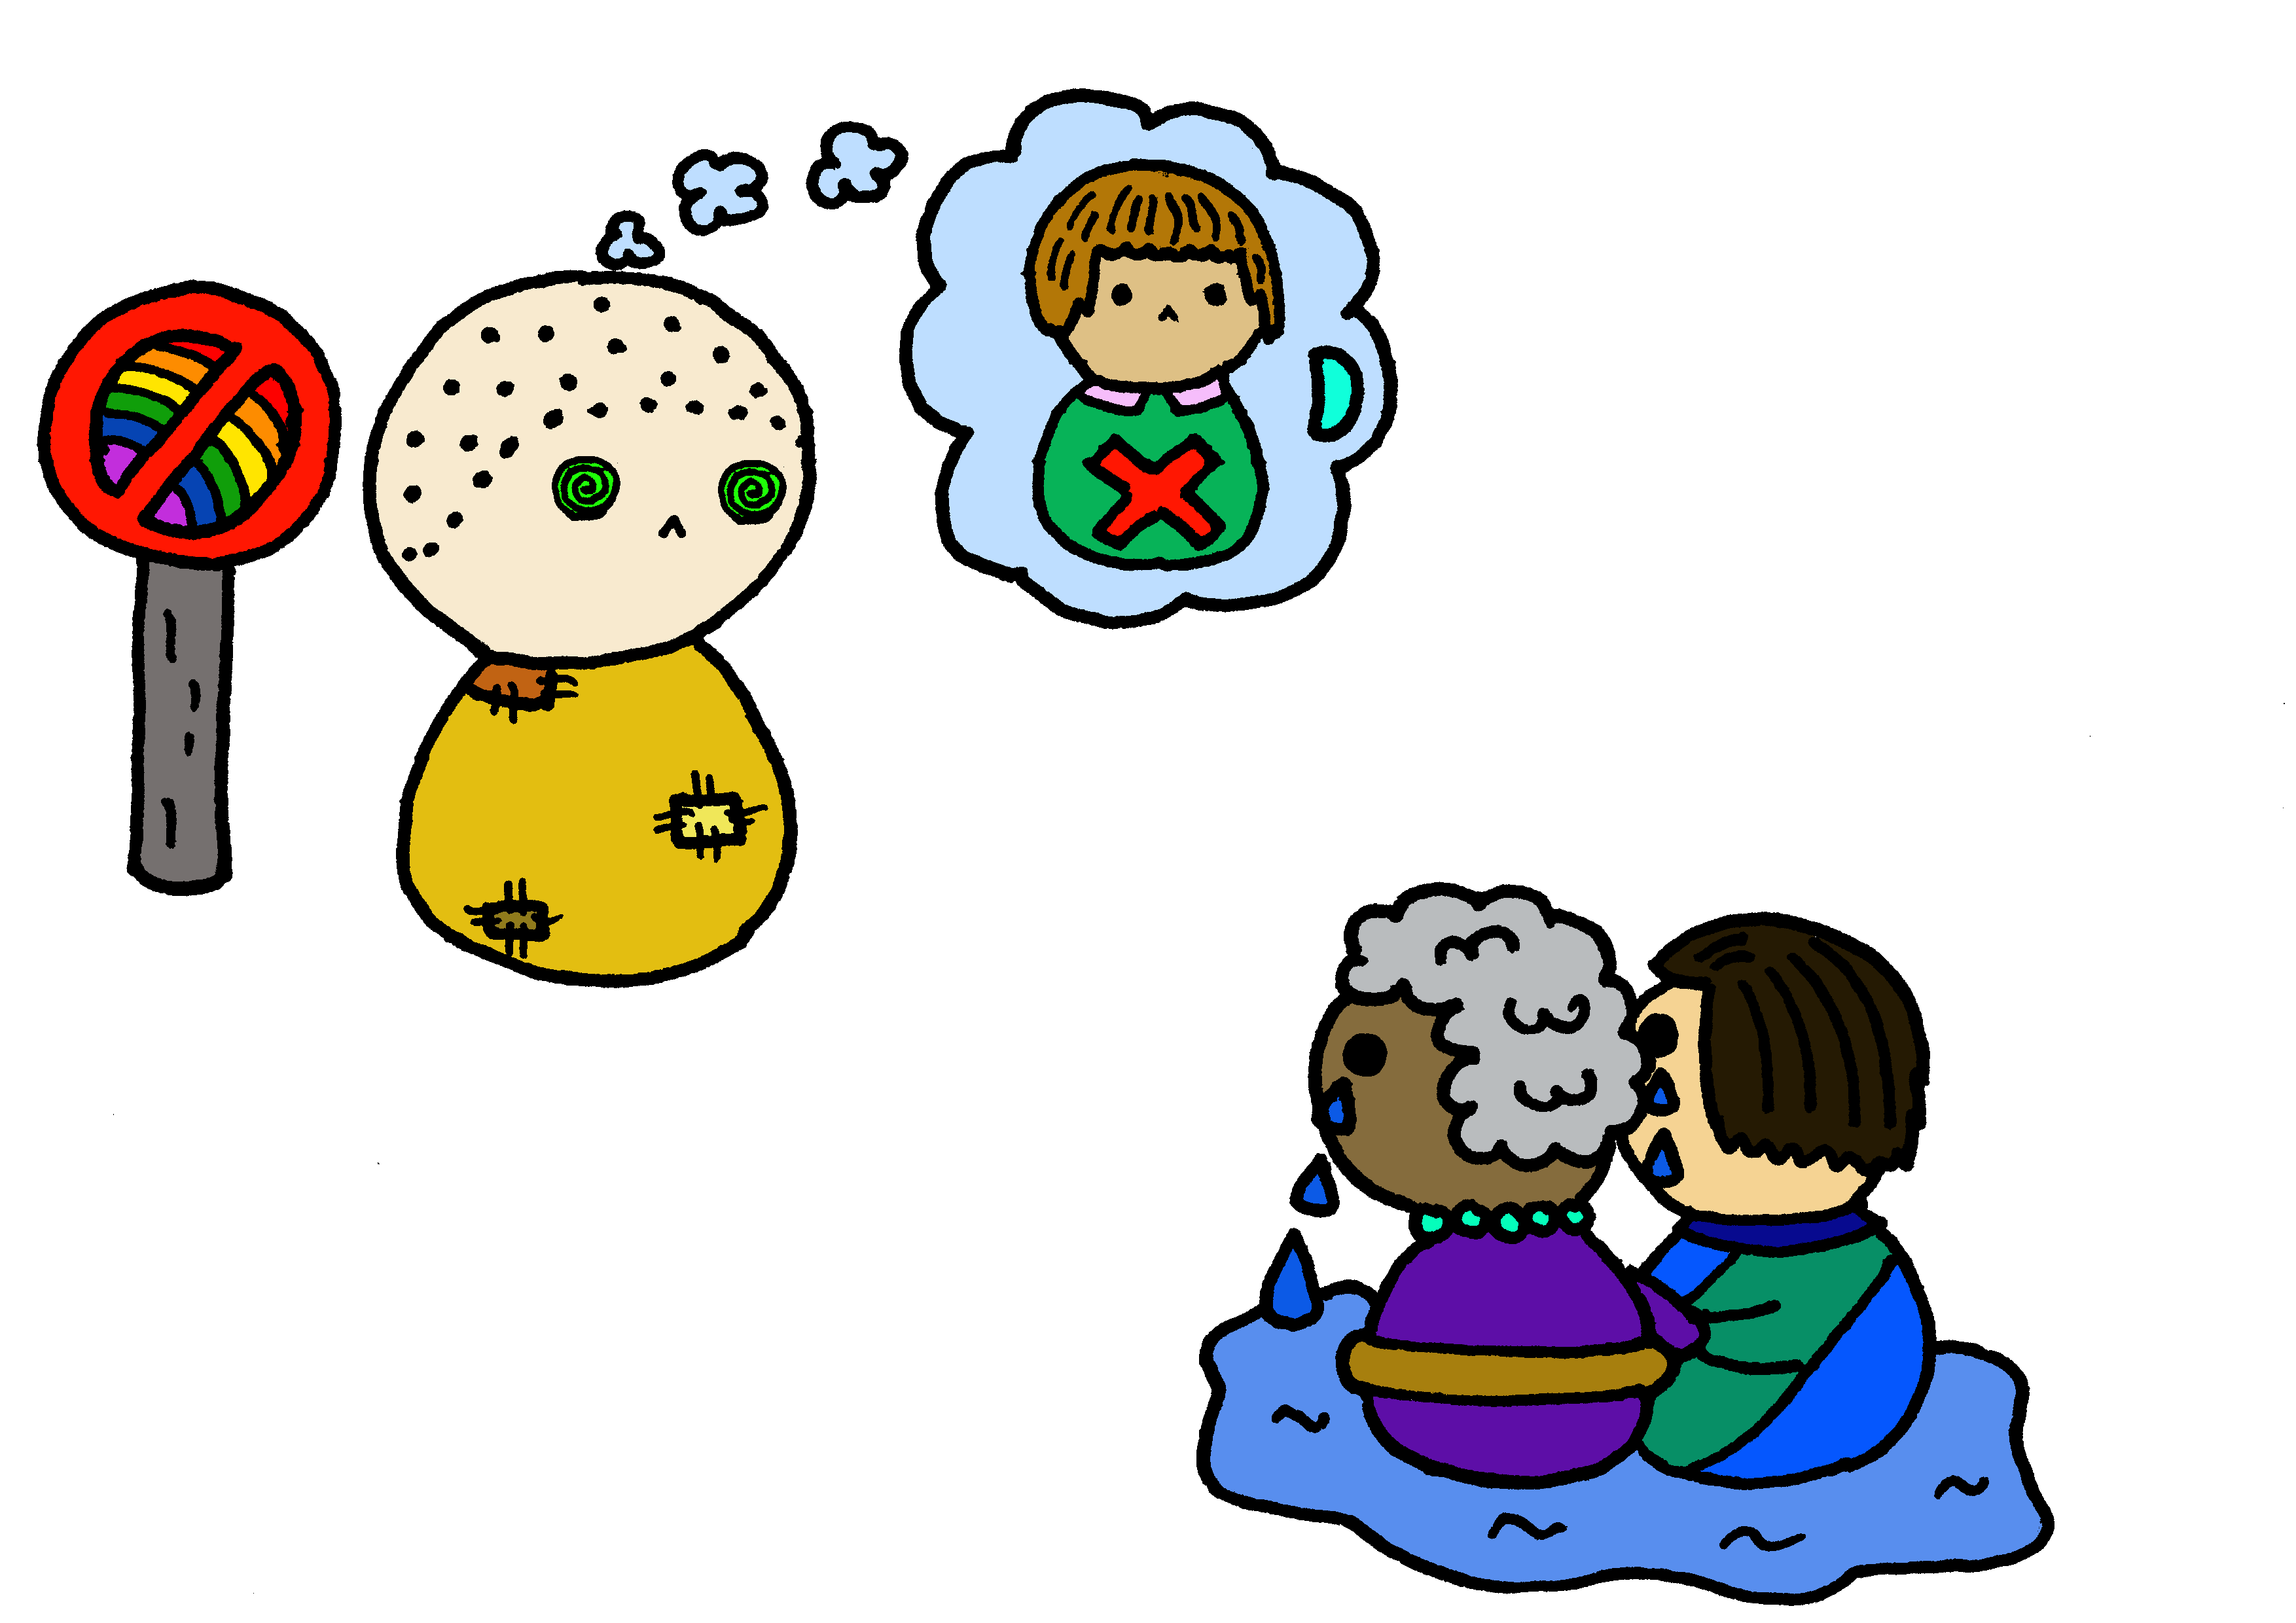
\includegraphics[width=0.6\paperwidth]{30.png}}
\end{figure}

\begin{quote}
\centering
\doublespacing
\textit{\Large \textcolor{red}{\textbf{Las opiniones de ciertas personas pueden crear prejuicios, intolerancia, fomentar la disriminación, la opresión, el odio y la violencia hacia la comunidad LGBTQIA+.}}}
\end{quote}

\chapter*{Opiniones dañinas}
\addcontentsline{toc}{chapter}{Opiniones dañinas}
\markboth{Darle la bienvenida al arcoíris}{Opiniones dañinas}

\phantomsection
\section*{La dolorosa realidad de la discriminación}
\addcontentsline{toc}{section}{La dolorosa realidad de la discriminación}

A pesar de que la mayor parte de la población LGBTQIA+ es feliz, las investigaciones muestran que una cantidad desproporcionada de personas de dicha comunidad sufren de mala salud mental y tienen una mayor tendencia a comportamientos suicidas. Esto está directamente vinculado a las experiencias de estigma, prejuicio, discriminación y abuso que sufren por ser parte de la comunidad LGBTQIA+.

Las personas LGBTQIA+ también sufren acoso, hostigamiento, abuso verbal y ataques violentos en muchos países. Por ello, es de suma importancia hablar sobre la discriminación y los prejuicios para así comprender los obstáculos que sufre la comunidad LGBTQIA+. Al hacerlo, podremos crear espacios seguros e incluyentes para todes.

\noindent\fbox{%
   \parbox{\textwidth}{%
\textit{\textbf{\Large \textcolor{white}{Algunos datos sobre la discriminación en contra de personas LGBTQIA+}}}

\textcolor{white}{\begin{itemize}
\setlength\itemsep{-0.3em}
\item 72 países criminalizan las relaciones sexuales consensuadas entre hombres.
\item 44 países criminalizan las relaciones sexuales consensuadas entre mujeres.
\item 11 países aplican la pena de muerte si una persona tiene relaciones sexuales consensuadas con otra persona de su mismo sexo.
\item 15 países criminalizan la identidad de género de las personas trans mediante leyes de `travestismo', `suplantación' o `de engaño'.
\item Alrededor del mundo, las personas intersexuales han sido forzadas a intervenciones médicas que violan tanto a sus derechos humanos como a su integridad corporal.
\end{itemize}}
   }
}

\phantomsection
\section*{Acotación sobre el no-yo}
\addcontentsline{toc}{section}{Acotación sobre el no-yo}

Algunes budistas acusan injustamente a les practicantes LGBTQIA+ de tener una `obsesión' o `apego' a la idea del `yo', usando a la doctrina budista del \textit{anatta} (no-yo) para insistir que estas identidades disidentes no son más que concepciones ilusorias y que no existen realmente. Mencionan también que enfocarnos en una identidad va en contra de las enseñanzas budistas; que esa es la razón por la cual las personas LGBTQIA+ sufren.

Es importante recalcar que ser queer, trans o intersexo es parte fundamental de la humanidad. El mero hecho de concebir a estas facetas como irreales e irrelevantes es caer en visiones erróneas y en un mal uso de la doctrina. Al hacerlo, negamos la realidad de las experiencias de vida de muchas personas, como sus relaciones, su comunidad o su trabajo. Este enfoque es dañino pues minimiza la discriminación, los prejuicios y la violencia tangible que las personas LGBTQIA+ sufren todos los días.

Algunes budistas usan el concepto del no-yo para silenciar a la comunidad LGBTQIA+ y que no hablen de los obstáculos, incluyendo el sufrimiento palpable, que les atañen. Las personas LGBTQIA+ sufren mayormente por la discriminación hacia su identidad. Es importante mencionar que ser parte de la comunidad LGBTQIA+ no es en sí una fuente o causa de sufrimiento, tal y como ser heterosexual o cisgénero tampoco es una fuente o causa de sufrimiento. Las personas LGBTQIA+ hablan sobre y mencionan sus identidades porque, a menudo, sufren por actitudes discriminatorias y buscan hacer un cambio en estos aspectos dañinos de la sociedad. Debemos celebrar la diversidad en lugar de ignorar y silenciarla.

or lo tanto, es vital que les budistas piensen cuidadosamente sobre cómo hablar sobre el no-yo, especialmente con aquelles que son oprimides por su identidad. De lo contrario y en lugar de ser una herramienta útil de crecimiento personal, el no-yo puede convertirse en un arma dañina, en un concepto de \textit{anatta} prejuicioso que podrá sentirse como  otro ataque injustificado en contra de la comunidad LGBTQIA+.

\subsubsection*{¿Cuál es tu identidad?}

Las personas LGBTQIA+ tienden a ser criticadas por hablar de los obstáculos que sufren y por tener una obsesión a sus identidades. Cuando hablamos del no-yo, es importante subrayar que las personas cisgénero y heterosexuales tamién tienen una sexualidad y un género. Puede que sea difícil de percibirlo así puesto que estos grupos tienden a autopercibirse como `normales' y porque la sociedad refuerza sus identidades sin darse cuenta.

Podríamos preguntarnos, pues:
\begin{wrapfigure}{l}{0.25\textwidth}
    \centering
    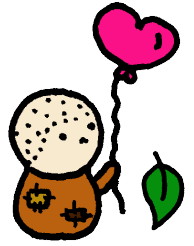
\includegraphics[width=0.25\textwidth]{33c.png}
\end{wrapfigure}
\begin{itemize}
\setlength\itemsep{-0.3em}
\item ¿Siempre escojo la misma opción de género en formatos?
\item ¿Me sentiría mal si alguien me menciona usando el género incorrecto?
\item ¿Le pediría a alguien que use mi nombre correcto si se equivocan?
\end{itemize}

¿Acaso esto significa que tengo una obsesión con mi identidad?

Podemos ser más empáticos:

\begin{itemize}
\setlength\itemsep{-0.3em}
\item ¿Cómo me sentiría si mi relación amorosa fuera criminalizada por el Estado?
\item ¿Qué sucedería si pierdo mi trabajo por razón de mi sexualidad o género?
\item ¿Alguna vez temí sufrir un ataque por demostrarle afecto a mi pareja en público?
\item ¿Lucharía por la igualdad de derechos si me trataran de estas maneras?
\end{itemize}

Independientemente de nuestra posición en el tema del `yo' y del `no-yo', las personas LGBTQIA+ siguen siendo oprimides y discriminades personalmente, socialmente y espiritualmente. Asegurémonos de no promover la opresión y no silenciemos diálogos en nuestras comunidades budistas sobre problemáticas que sufre la comunidad LGBTQIA+,

También es importante mencionar que hay ciertos aspectos del `yo' con los cuales les budistas buscan fervientemente identificarse, como la generosidad, la conducta ética, la amabilidad, la compasión y la sabiduría.

\phantomsection
\section*{Experiencias interseccionales: etnia, género y sexualidad}
\addcontentsline{toc}{section}{Experiencias interseccionales: etnia, género y sexualidad}

La población LGBTQIA+ es víctima de racismo, clasismo, capacitismo y otros tipos de prejuicios y discriminación. El término `interseccionalidad' se refiere a la comprensión de cómo puede haber una combinación de identidades (como la etnia, el género, la sexualidad, las capacidades motrices y/o cognitivas, el nivel socioeconómico, el nivel de educación escolar, la ubicación geográfica…) y cómo estas pueden conllevar discriminación y/o privilegios en la sociedad. Veamos algunos ejemplos: una mujer trans negra tendrá una experiencia completamente distinta en un centro budista occidental a la de un hombre blanco cisgénero. De igual manera, en un monasterio, la experiencia de un hombre cisgénero gay será totalmente distinta a la de una mujer blanca cisgénero heterosexual.

Si identificamos cómo estas diversas identidades pueden yuxtaponerse, podemos ser más conscientes de cómo existe una interseccionalidad entre la discriminación y el privilegio, incluso para aquellas personas que comparten ciertas identidades. Es de suma importancia entender estas diferencias puesto que demuestran que las experiencias de cada quien son distintas y que, por ello, se necesitan diversos enfoques para promover la inclusión y la equidad para las disidencias de nuestras comunidades.

\begin{figure}[h]
    \centering
    \makebox[0pt]{%
    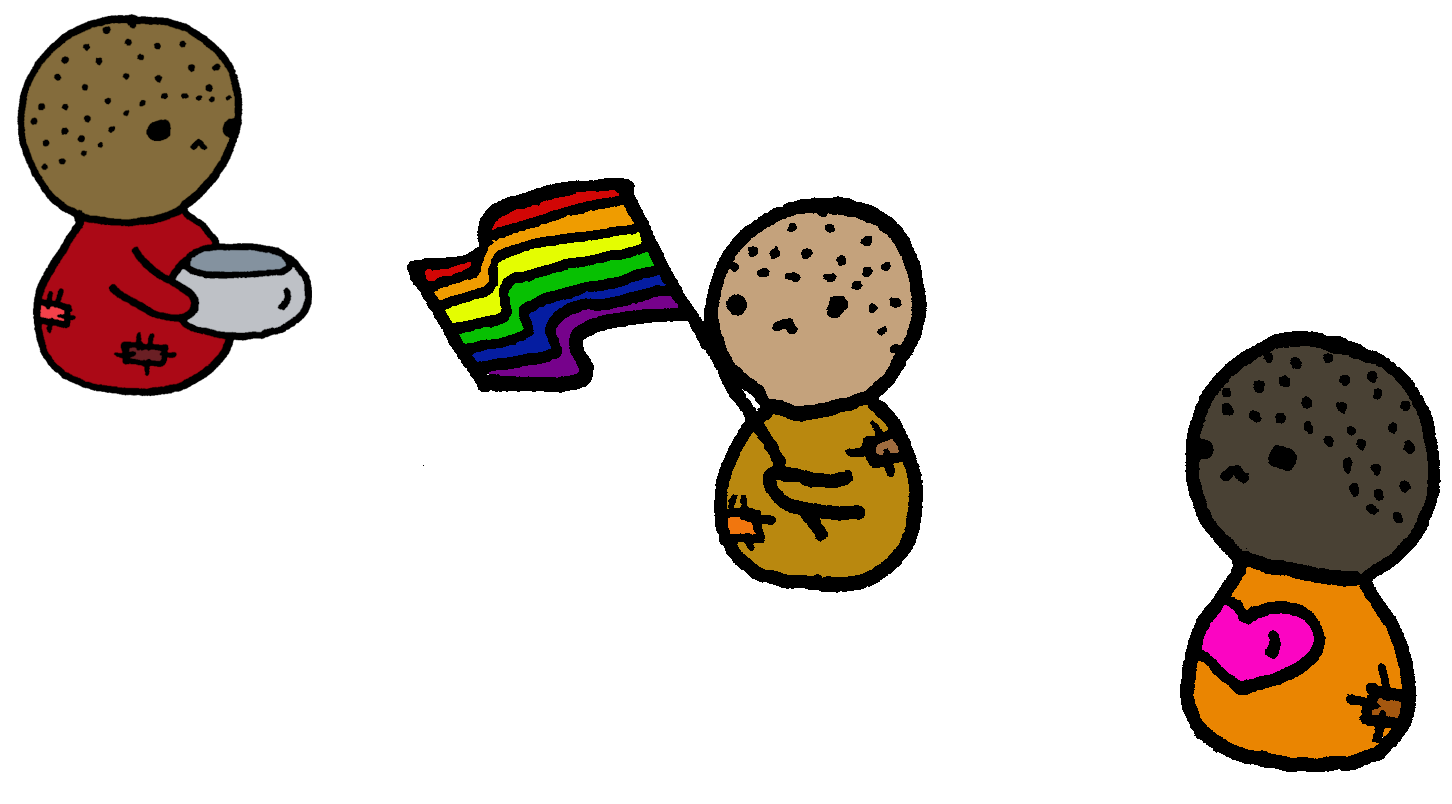
\includegraphics[width=0.5\paperwidth]{13c.png}}
\end{figure}

\begin{quote}
\centering
\textit{\Large \textcolor{red}{\textbf{Es fundamental reconocer aquello que nos diferencia y que no todes somos iguales}}}
\end{quote}

\newpage
\thispagestyle{empty}
\begin{quote}
\centering
\doublespacing
\textit{\Large \textcolor{purple}{\textbf{Existe una gran diversidad dentro de la misma comunidad LGBTQIA+: personas, relaciones, familias, amistades, subculturas ¡y mucho más!}}}
\end{quote}

\begin{figure}[h]
    \centering
    \makebox[0pt]{%
    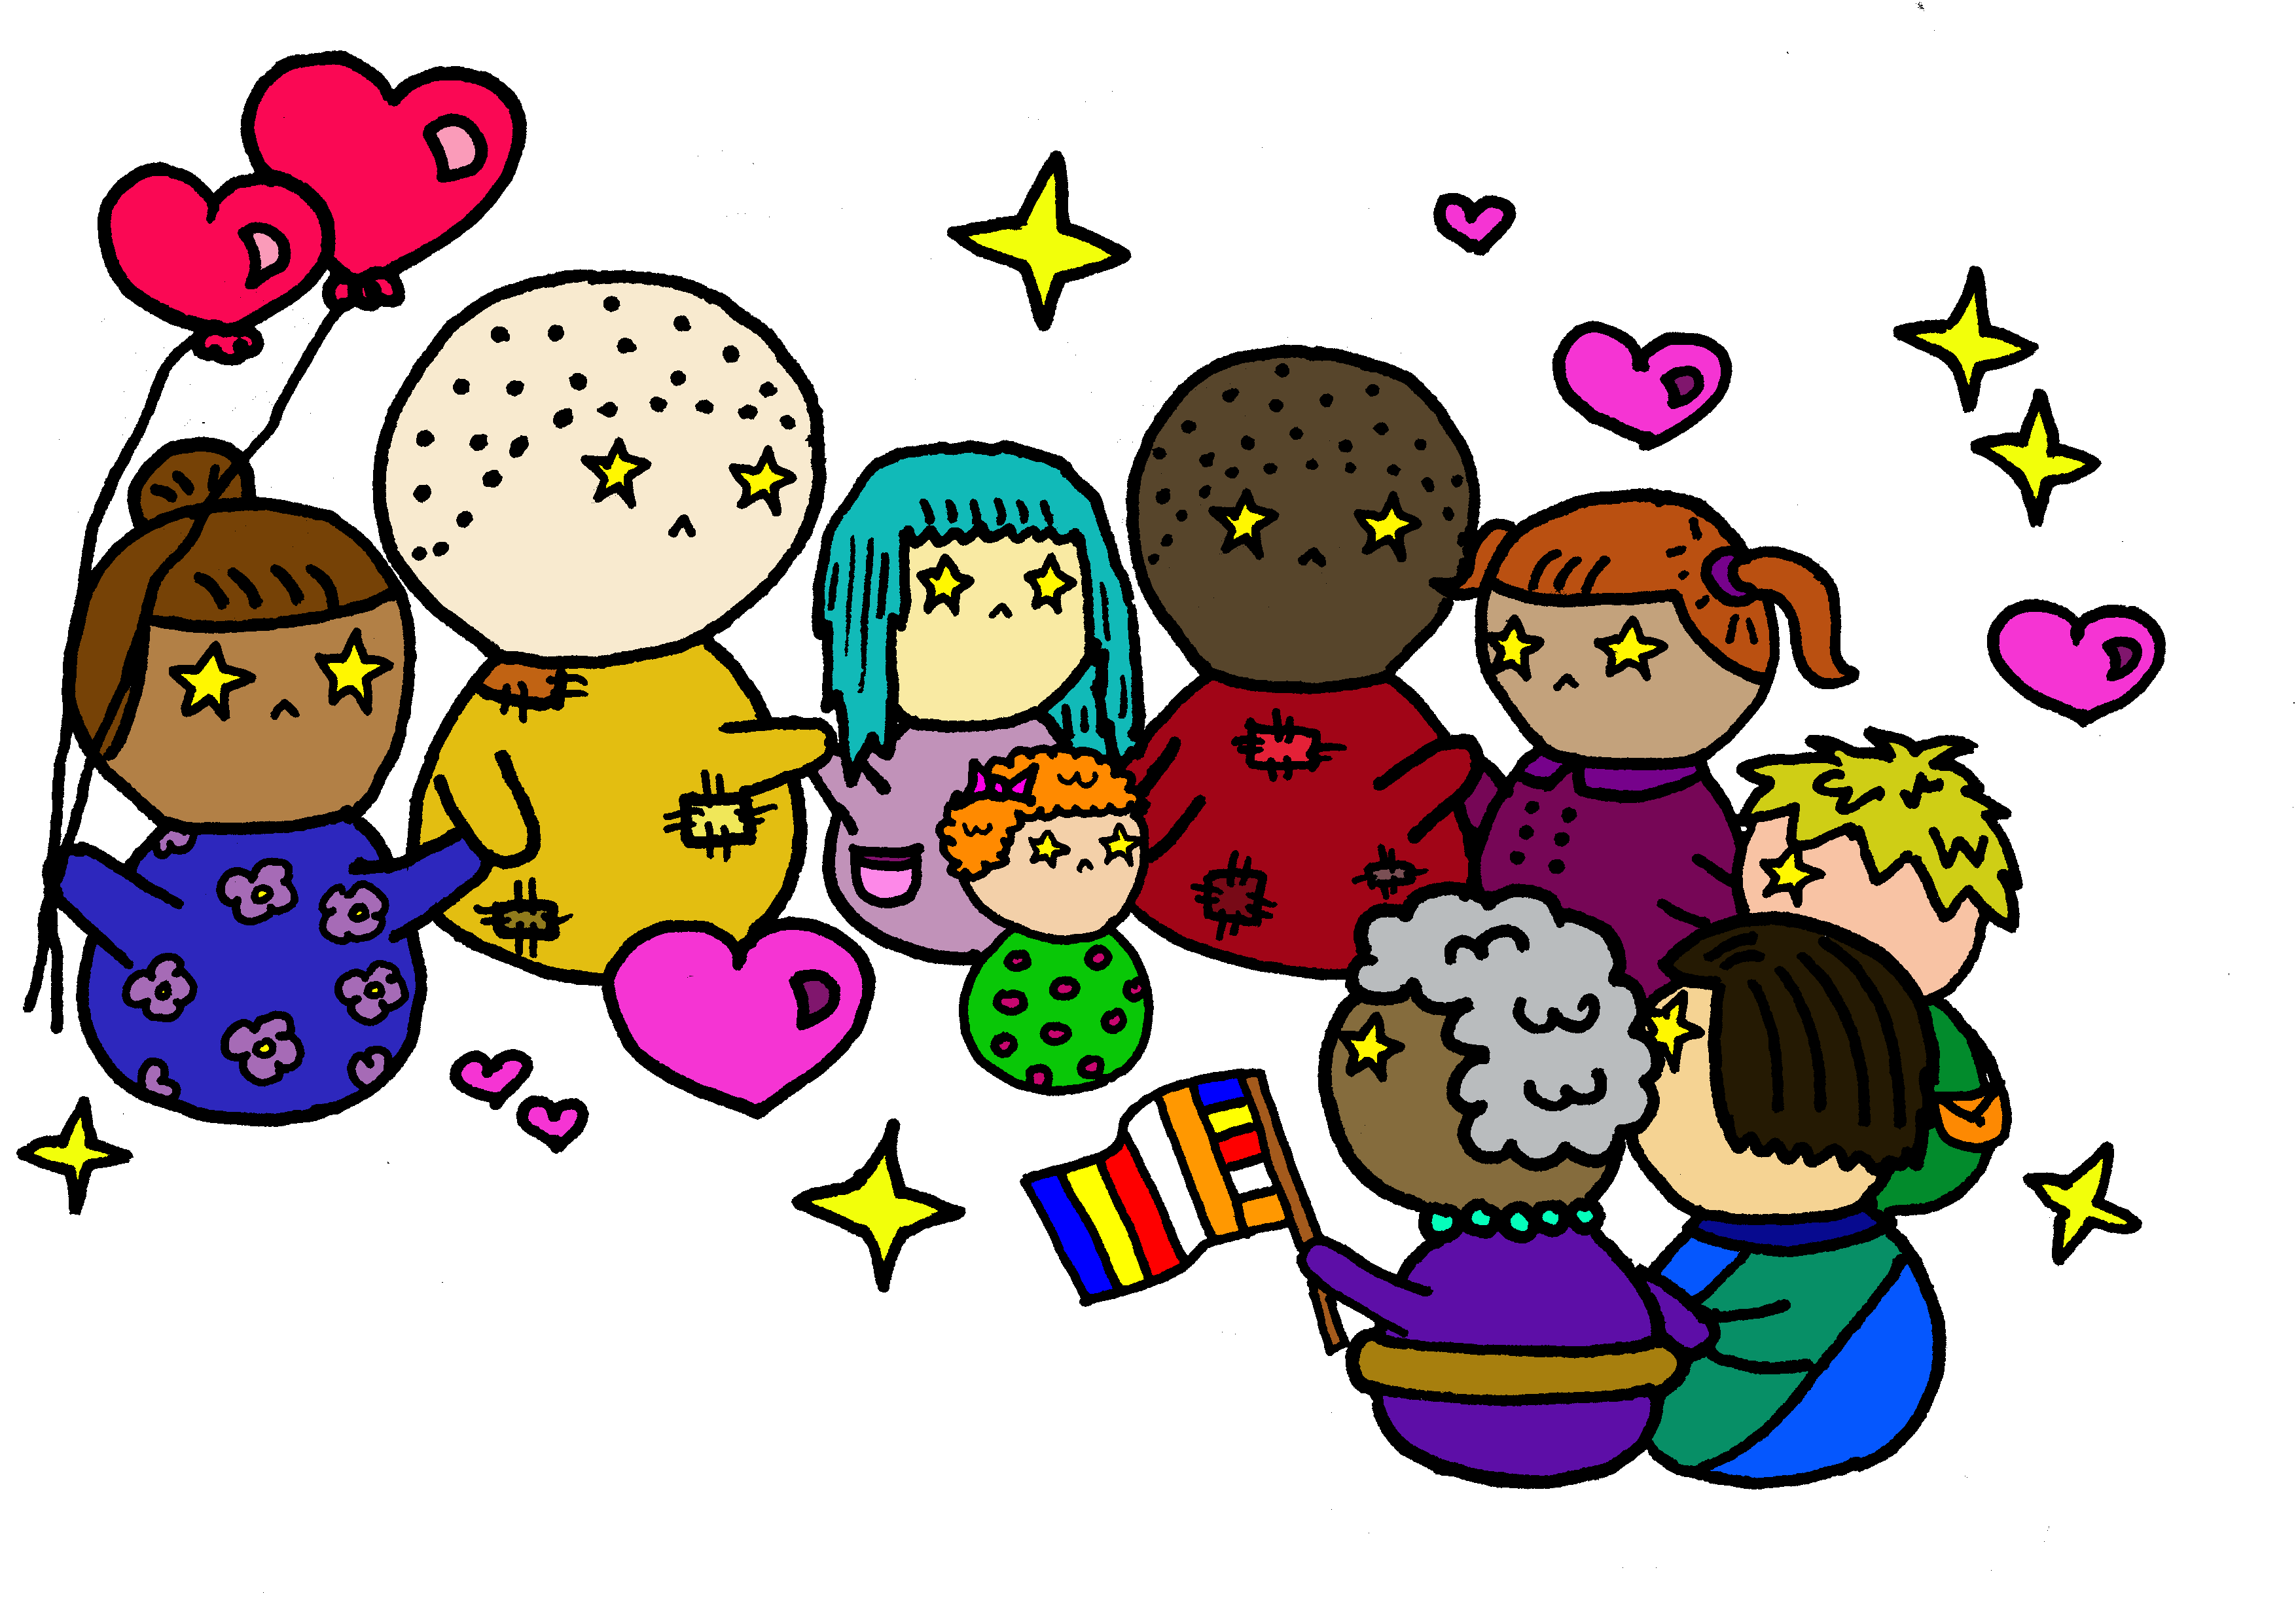
\includegraphics[width=0.9\paperwidth]{36-37.png}}
\end{figure}

\chapter*{Guía sobre las personas con experiencia de vida LGBTQIA+}
\addcontentsline{toc}{chapter}{Guía sobre las personas con experiencia de vida LGBTQIA+}
\markboth{Darle la bienvenida al arcoíris}{Guía sobre las personas con experiencia de vida LGBTQIA+}

\phantomsection
\section*{El cuerpo, la identidad de género y la sexualidad son temas que no deben confundirse}
\addcontentsline{toc}{section}{El cuerpo, la identidad de género y la sexualidad son temas que no deben confundirse}

Todes tenemos un cuerpo, una sexualidad y una identidad de género. Es vital tener, por lo menos, una comprensión básica sobre algunos conceptos y términos para entender los problemas que sufre la comunidad LGBTQIA+.

\subsubsection*{El cuerpo y las características sexuales}

Todos los cuerpos cuentan con características únicas, como la forma, la talla, entre otras. Esto incluye a las diferentes características sexuales, como los elementos físicos relacionados al desarrollo corporal, la regulación hormonal y el sistema reproductivo. Las características sexuales primarias incluyen a las gónadas, los cromosomas, los genitales y las hormonas, mientras que las secundarias surgen durante la pubertad, y pueden incluir el tejido mamario, el cambio de la voz, y el crecimiento de vello facial y púbico.

Ya que los órganos corporales no son lo que define nuestro género, es mejor usar el término `características sexuales' en lugar de `sexo biológico', `hombre biológico' o `mujer biológica'. A pesar de lo que se nos ha enseñado —que existen únicamente cuerpos de hombre y de mujer—, existe una gran diversidad de cuerpos distintos.

\begin{figure}[h]
    \centering
    \makebox[0pt]{%
    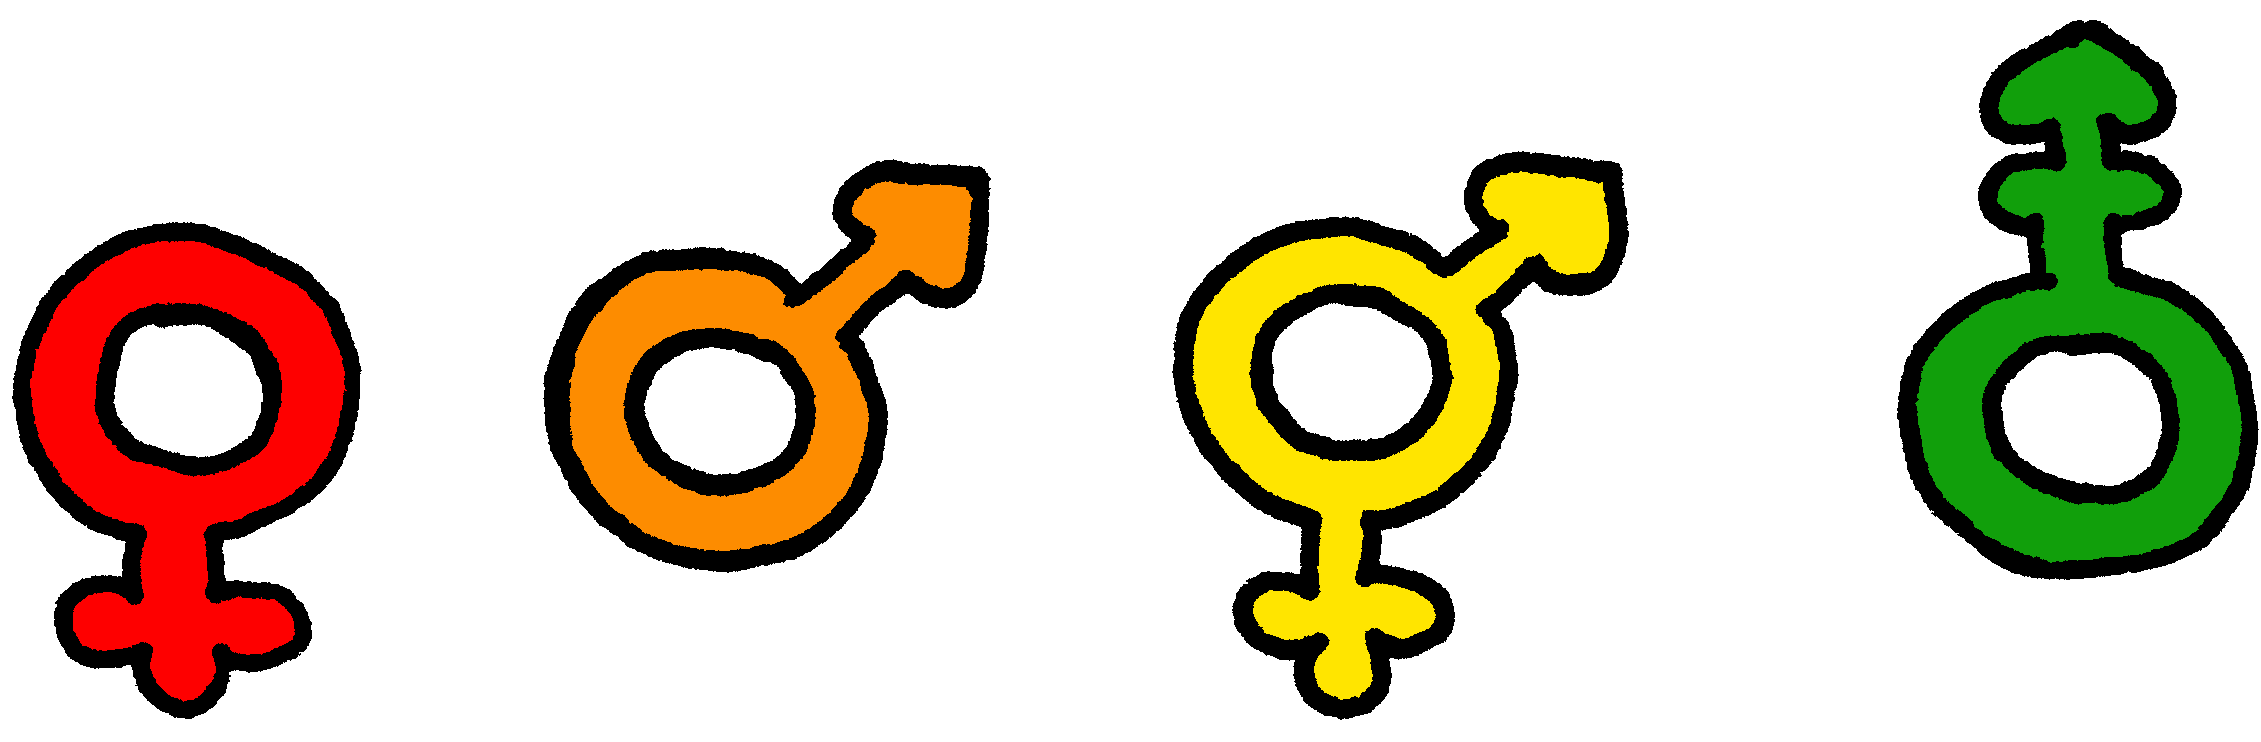
\includegraphics[width=0.5\paperwidth]{38-39c.png}}
\end{figure}

\subsubsection*{El cuerpo y el género}

El cuerpo y el género son conceptos distintos; tener un tipo de cuerpo no significa que te debas identificar con un género específico, ya que cualquier persona, sin importar su cuerpo, puede identificarse con cualquier género.

El género (hombre, mujer, ninguno de de estos, una combinación de ambos o algo totalmente distinto) es una parte de nuestra identidad. La relación que alguien tiene con su género puede cambiar con el tiempo.

\subsubsection*{Sexo asignado al nacer}

Se nos asignó un sexo un sexo a la mayor parte de nosotres, y este fue cimentado todavía más por las personas a nuestro alrededor durante nuestra infancia y adolescencia. Muches se identifican con el sexo que se les asignó al nacer, pero otres no. 

\subsubsection*{Cisgénero}

El término `cisgénero' o `cis' (que en latín significa ‘de este lado’) en un término que se usa para referirse a aquellas personas que se identifican con el sexo que se les asignó al nacer. Por ejemplo, una persona a la que se le asignó `hombre' al nacer y que se identifica como tal es un hombre cis.

\begin{figure}[h]
    \centering
    \makebox[0pt]{%
    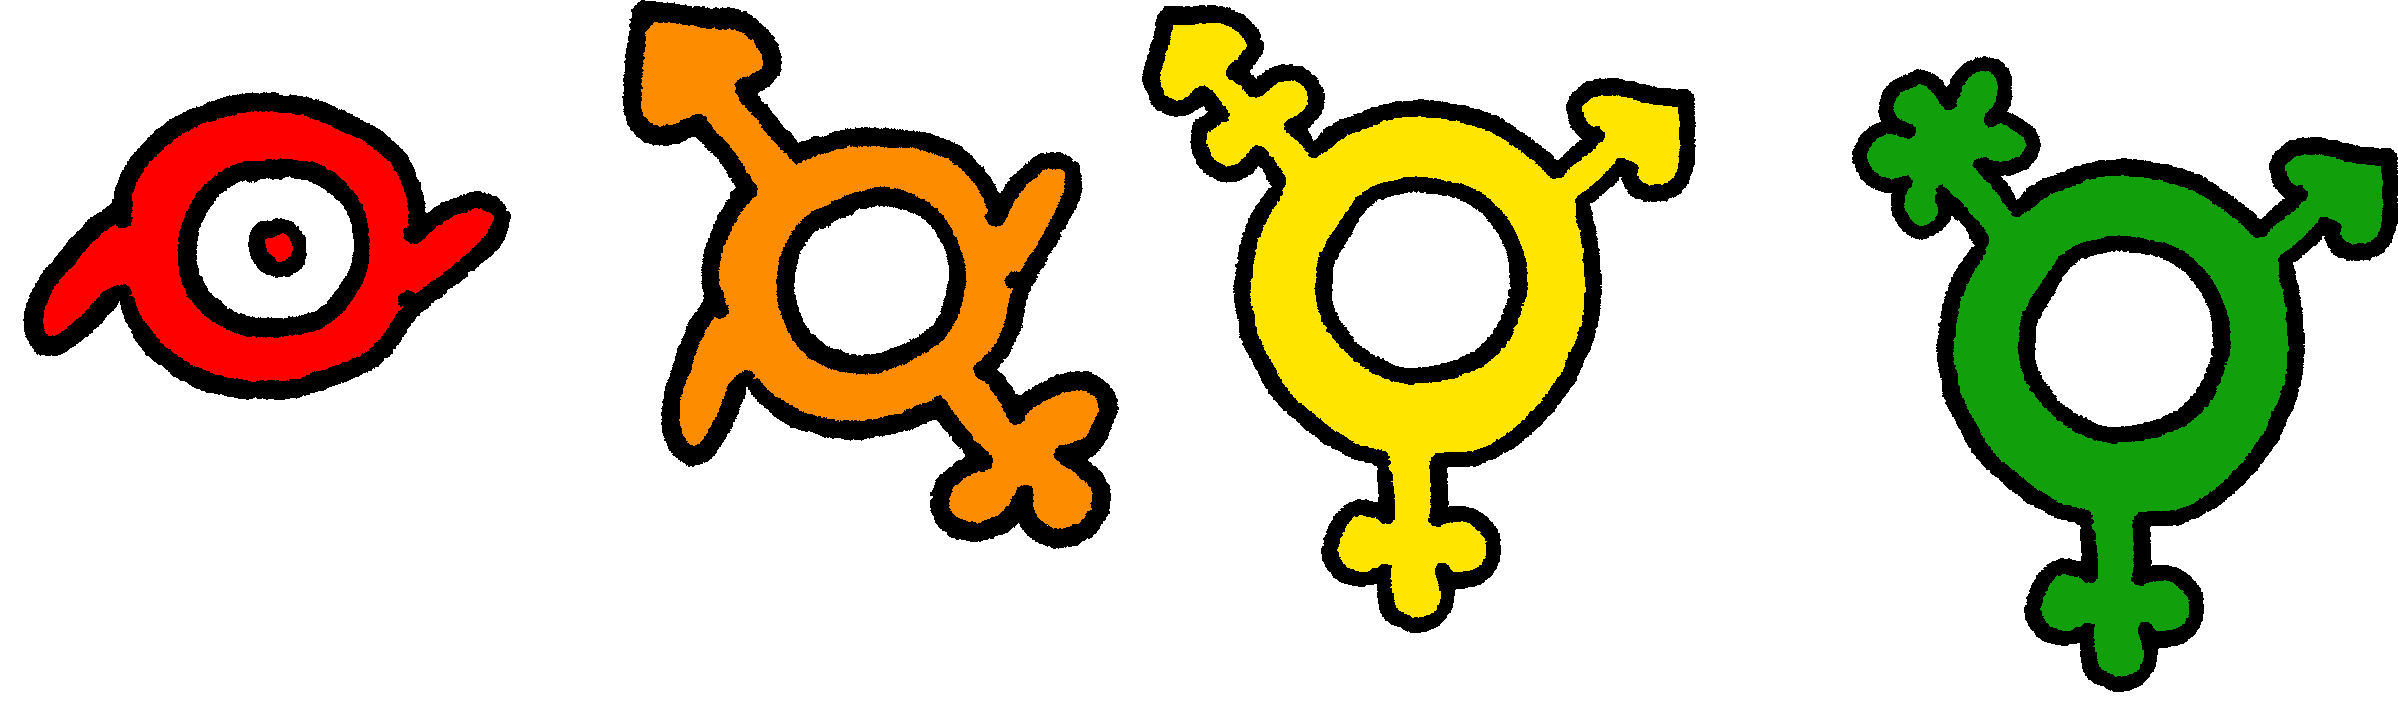
\includegraphics[width=0.5\paperwidth]{38-39c3.png}}
\end{figure}

\subsubsection*{Transgénero}

El término `transgénero',  `trans' o `género diverso' designa aquellas personas que no se identifican parcial o completamente con el sexo que se les asignó al nacer; designa una identidad de género, no una orientación sexual.

\subsubsection*{Orientación sexual}

El término `orientación sexual' o `sexualidad' se refiere a la atracción o falta de la misma que tengamos hacia les demás. Ni nuestro cuerpo ni nuestras características sexuales ni nuestra identidad de género tienen que ver con la orientación sexual que tengamos. La sexualidad es un espectro y puede cambiar con el tiempo.

\begin{figure}[h]
    \centering
    \makebox[0pt]{%
    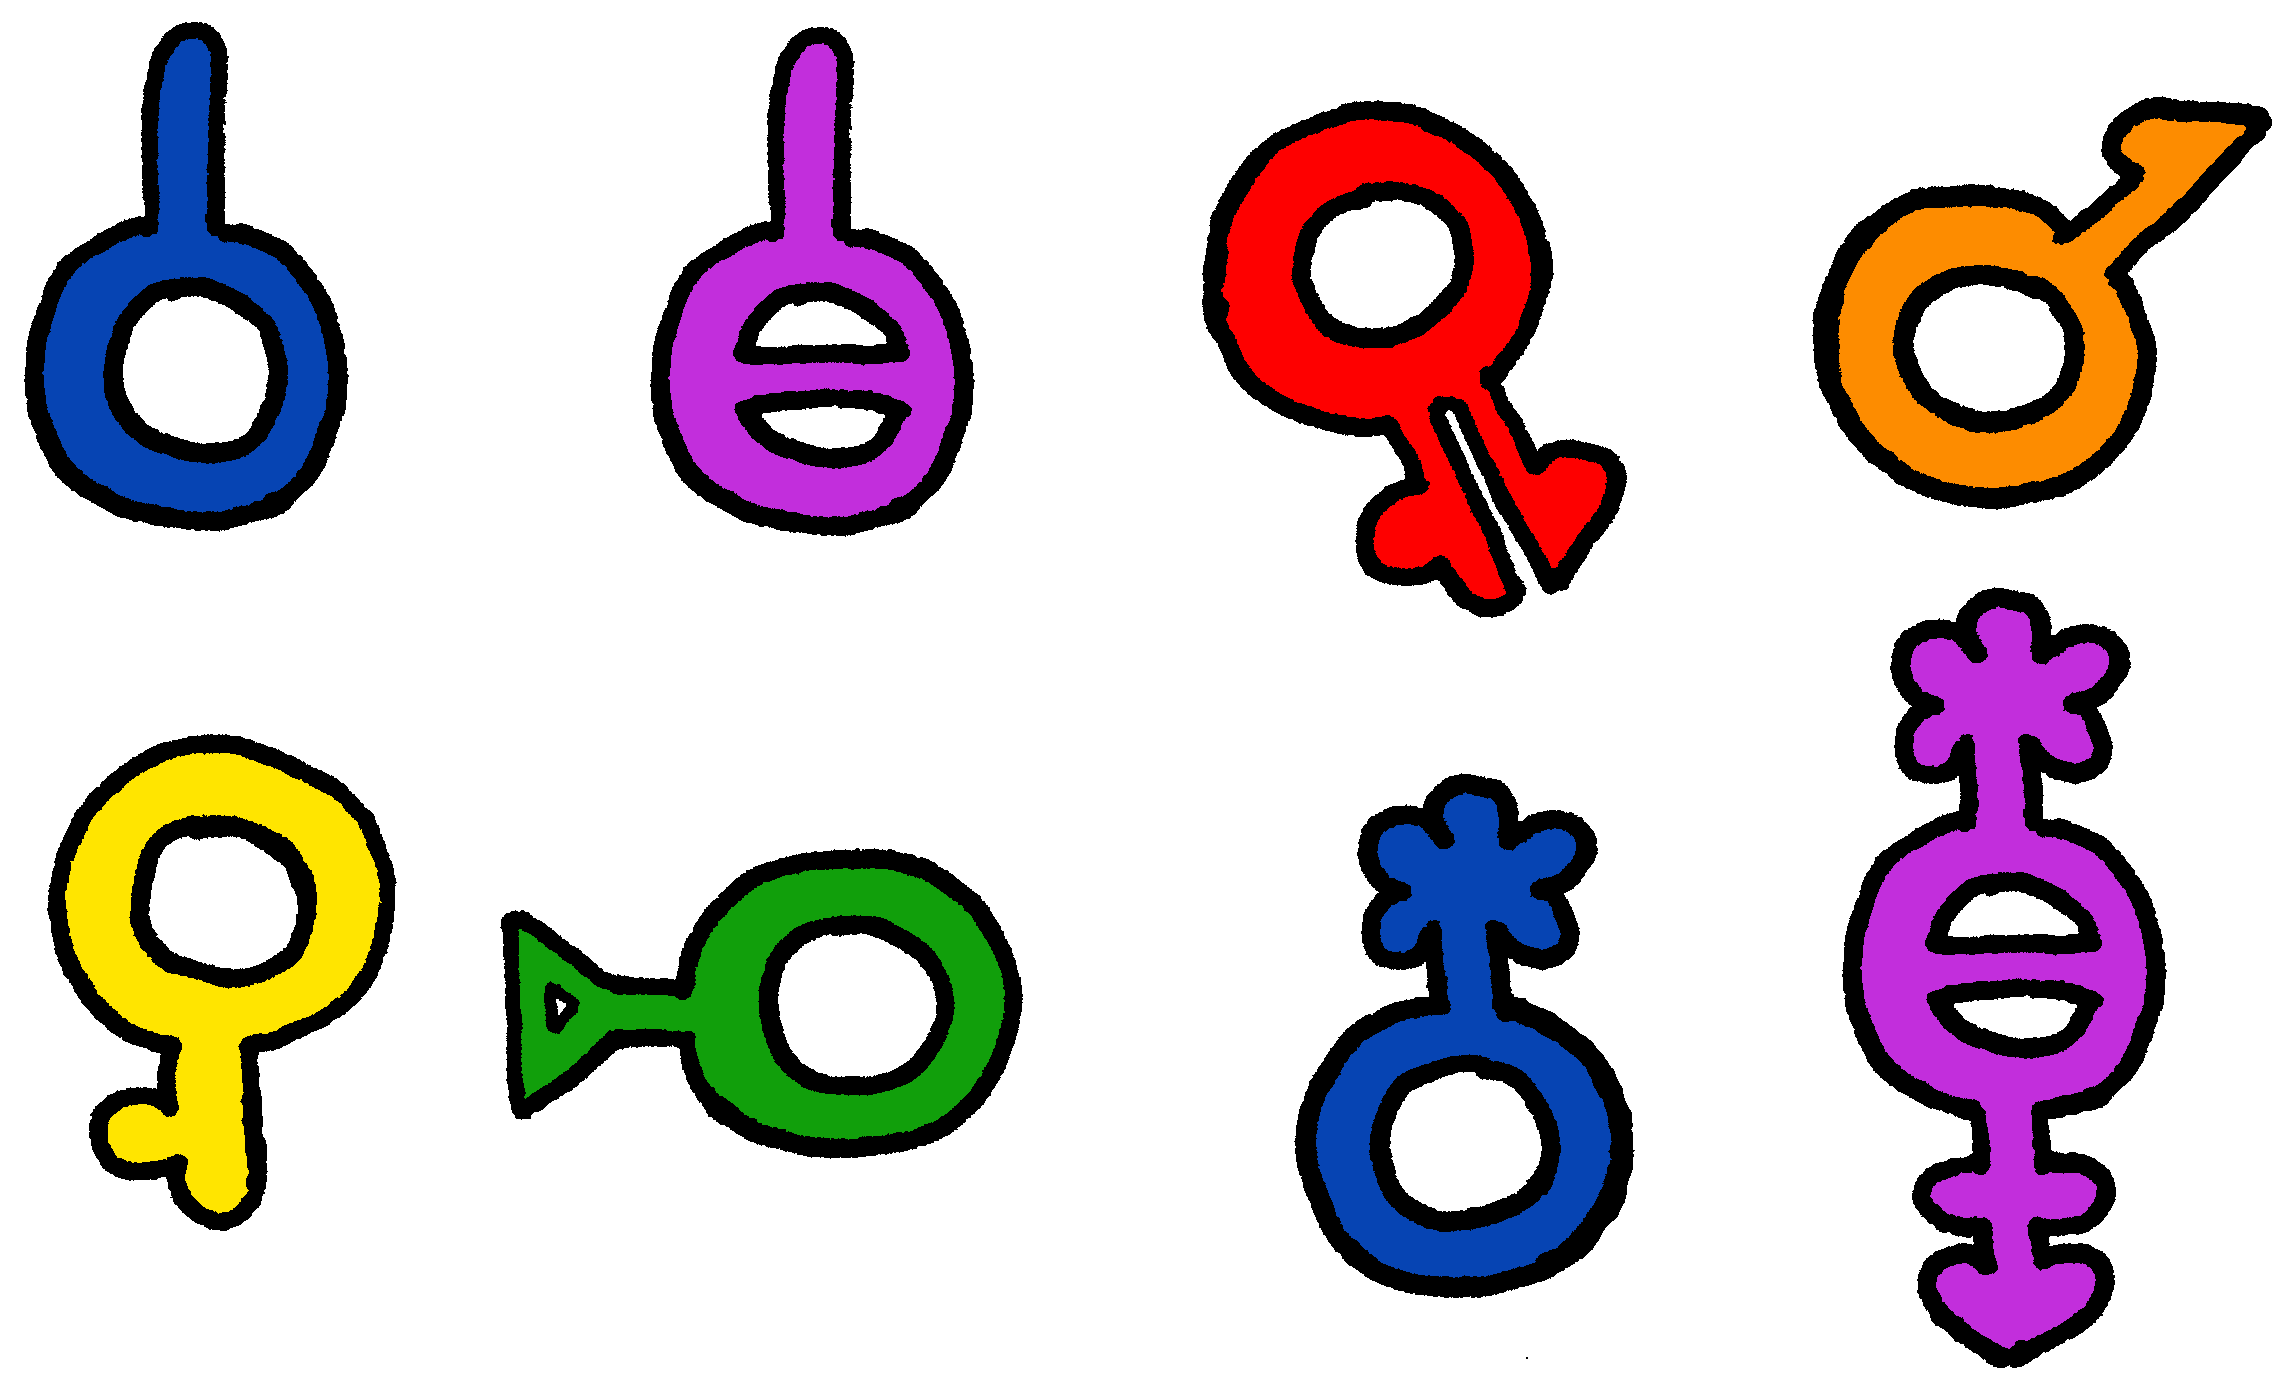
\includegraphics[width=0.5\paperwidth]{38-39c2.png}}
\end{figure}

\phantomsection
\section*{Intersexualidad}
\addcontentsline{toc}{section}{Intersexualidad}

El término `intersexualidad' es un hiperónimo que designa a aquellas personas que tienen variaciones naturales de aquello que concebimos  como cuerpos `de hombre' o `de mujer' tradicionales. Aproximadamente, el 1.7 \% de la población mundial tiene características intersexuales como características genitales, cromosómicas o físicas, las cuales pueden ser visibles durante la etapa de gestación, al momento de nacer, durante la pubertad o en la etapa adulta (por ejemplo, si se busca concebir une hije). Cada una de estas características puede variar en su nivel de expresión.

Muchas personas intersexuales se identifican con el sexo que se les asignó al nacer —hombre o mujer—, pero otras se identifican de otra forma. Ciertas personas intersexuales no se identifican con el sexo que se les asignó al nacer, pero tampoco se consideran a sí mismas como transgénero, mientras que otras sí se identifican como tal. 

Las posibilidades de identidades son las mismas tanto para personas intersexuales como para las no-intersexuales; algunes se identifican como LGBT, pero otres no. La intersexualidad no está relacionada a la identidad de género (no es lo mismo que identificarse como transgénero o como género no binario) ni a la sexualidad (una persona intersexual puede ser lesbiana, gay, bisexual, heterosexual…).

\begin{figure}[h]
    \centering
    \makebox[0pt]{%
    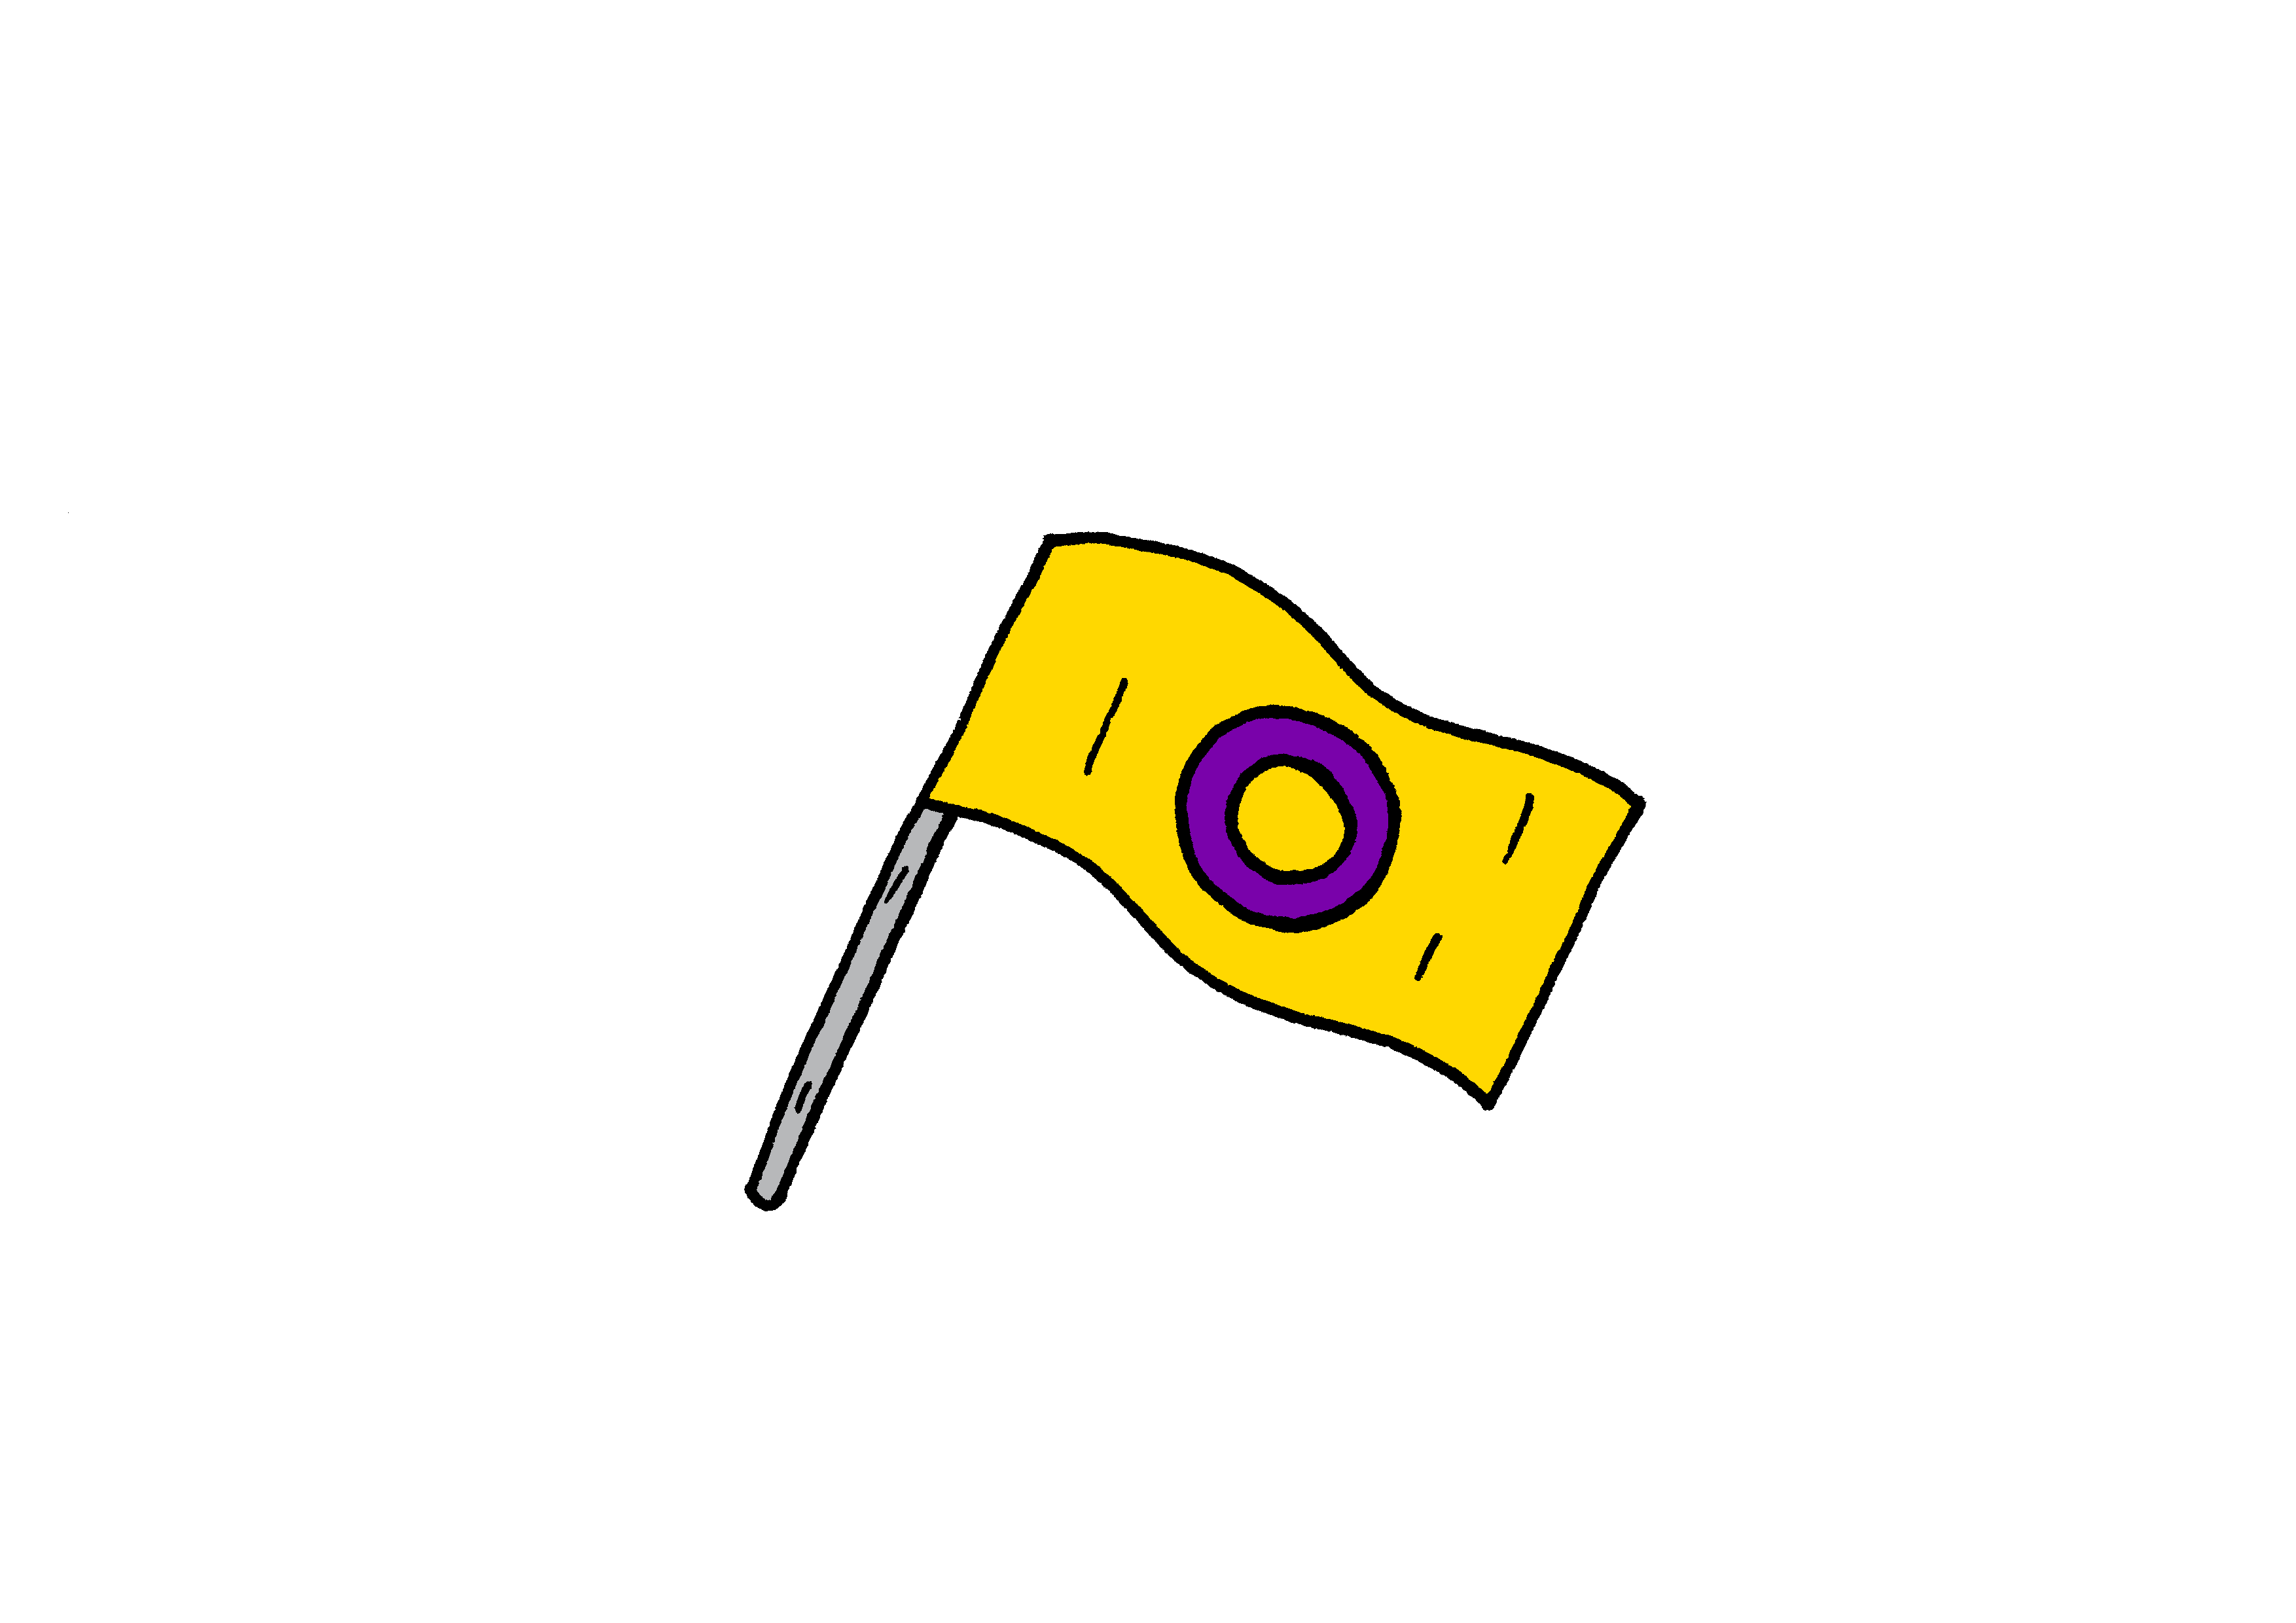
\includegraphics[width=0.6\paperwidth]{41.png}}
\end{figure}

\noindent\fbox{%
    \parbox{\textwidth}{%
\textit{\textbf{\Large \textcolor{white}{Estas son algunas realidades que lastiman a las personas intersexuales}}}

\textcolor{white}{\begin{itemize}
\setlength\itemsep{-0.3em}
\item La falta de reconocimiento pleno de la autonomía corporal y de los derechos humanos de las personas intersexuales.
\item La cirugía no consensuada y la toma de hormonas para que las infancias intersexuales para categorizarles como hombres o mujeres que busca invisibilizarles.
\item La estigmatización y el acoso social a los cuerpos en entornos educativos, deportivos, laborales y médicos, entre otros.
\item El uso de lenguaje arcaico (e. g. `hermafrodita') ofensivo y errado, o referirse a la intersexualidad como `un enfermedad', puesto que no lo es.
\end{itemize}}
    }%
}

\phantomsection
\section*{Personas trans y de género diverso}
\addcontentsline{toc}{section}{Personas trans y de género diverso}

Tanto el término `trans' como `género diverso' son hiperónimos que abarcan a aquellas personas que no se identifican con el sexo que se les asignó al nacer. Algunas ven al término `trans' como una experiencia o un antecedente en lugar de una identidad en sí; se identifican, pues, únicamente como hombres, mujeres o personas no binarias, mientras que otras personas se identifican específicamente como hombres o mujeres trans.

El término `género diverso' abarca a todas las formas de género posible en la comunidad LGBTQIA+: a personas que se identifican como transgénero, a aquellas que dudan de su identidad de género, a quienes no se identifican ni como hombre ni como mujer, a personas no binarias, y a aquellas que tienen un género fluido.

\begin{figure}[h]
    \centering
    \makebox[0pt]{%
    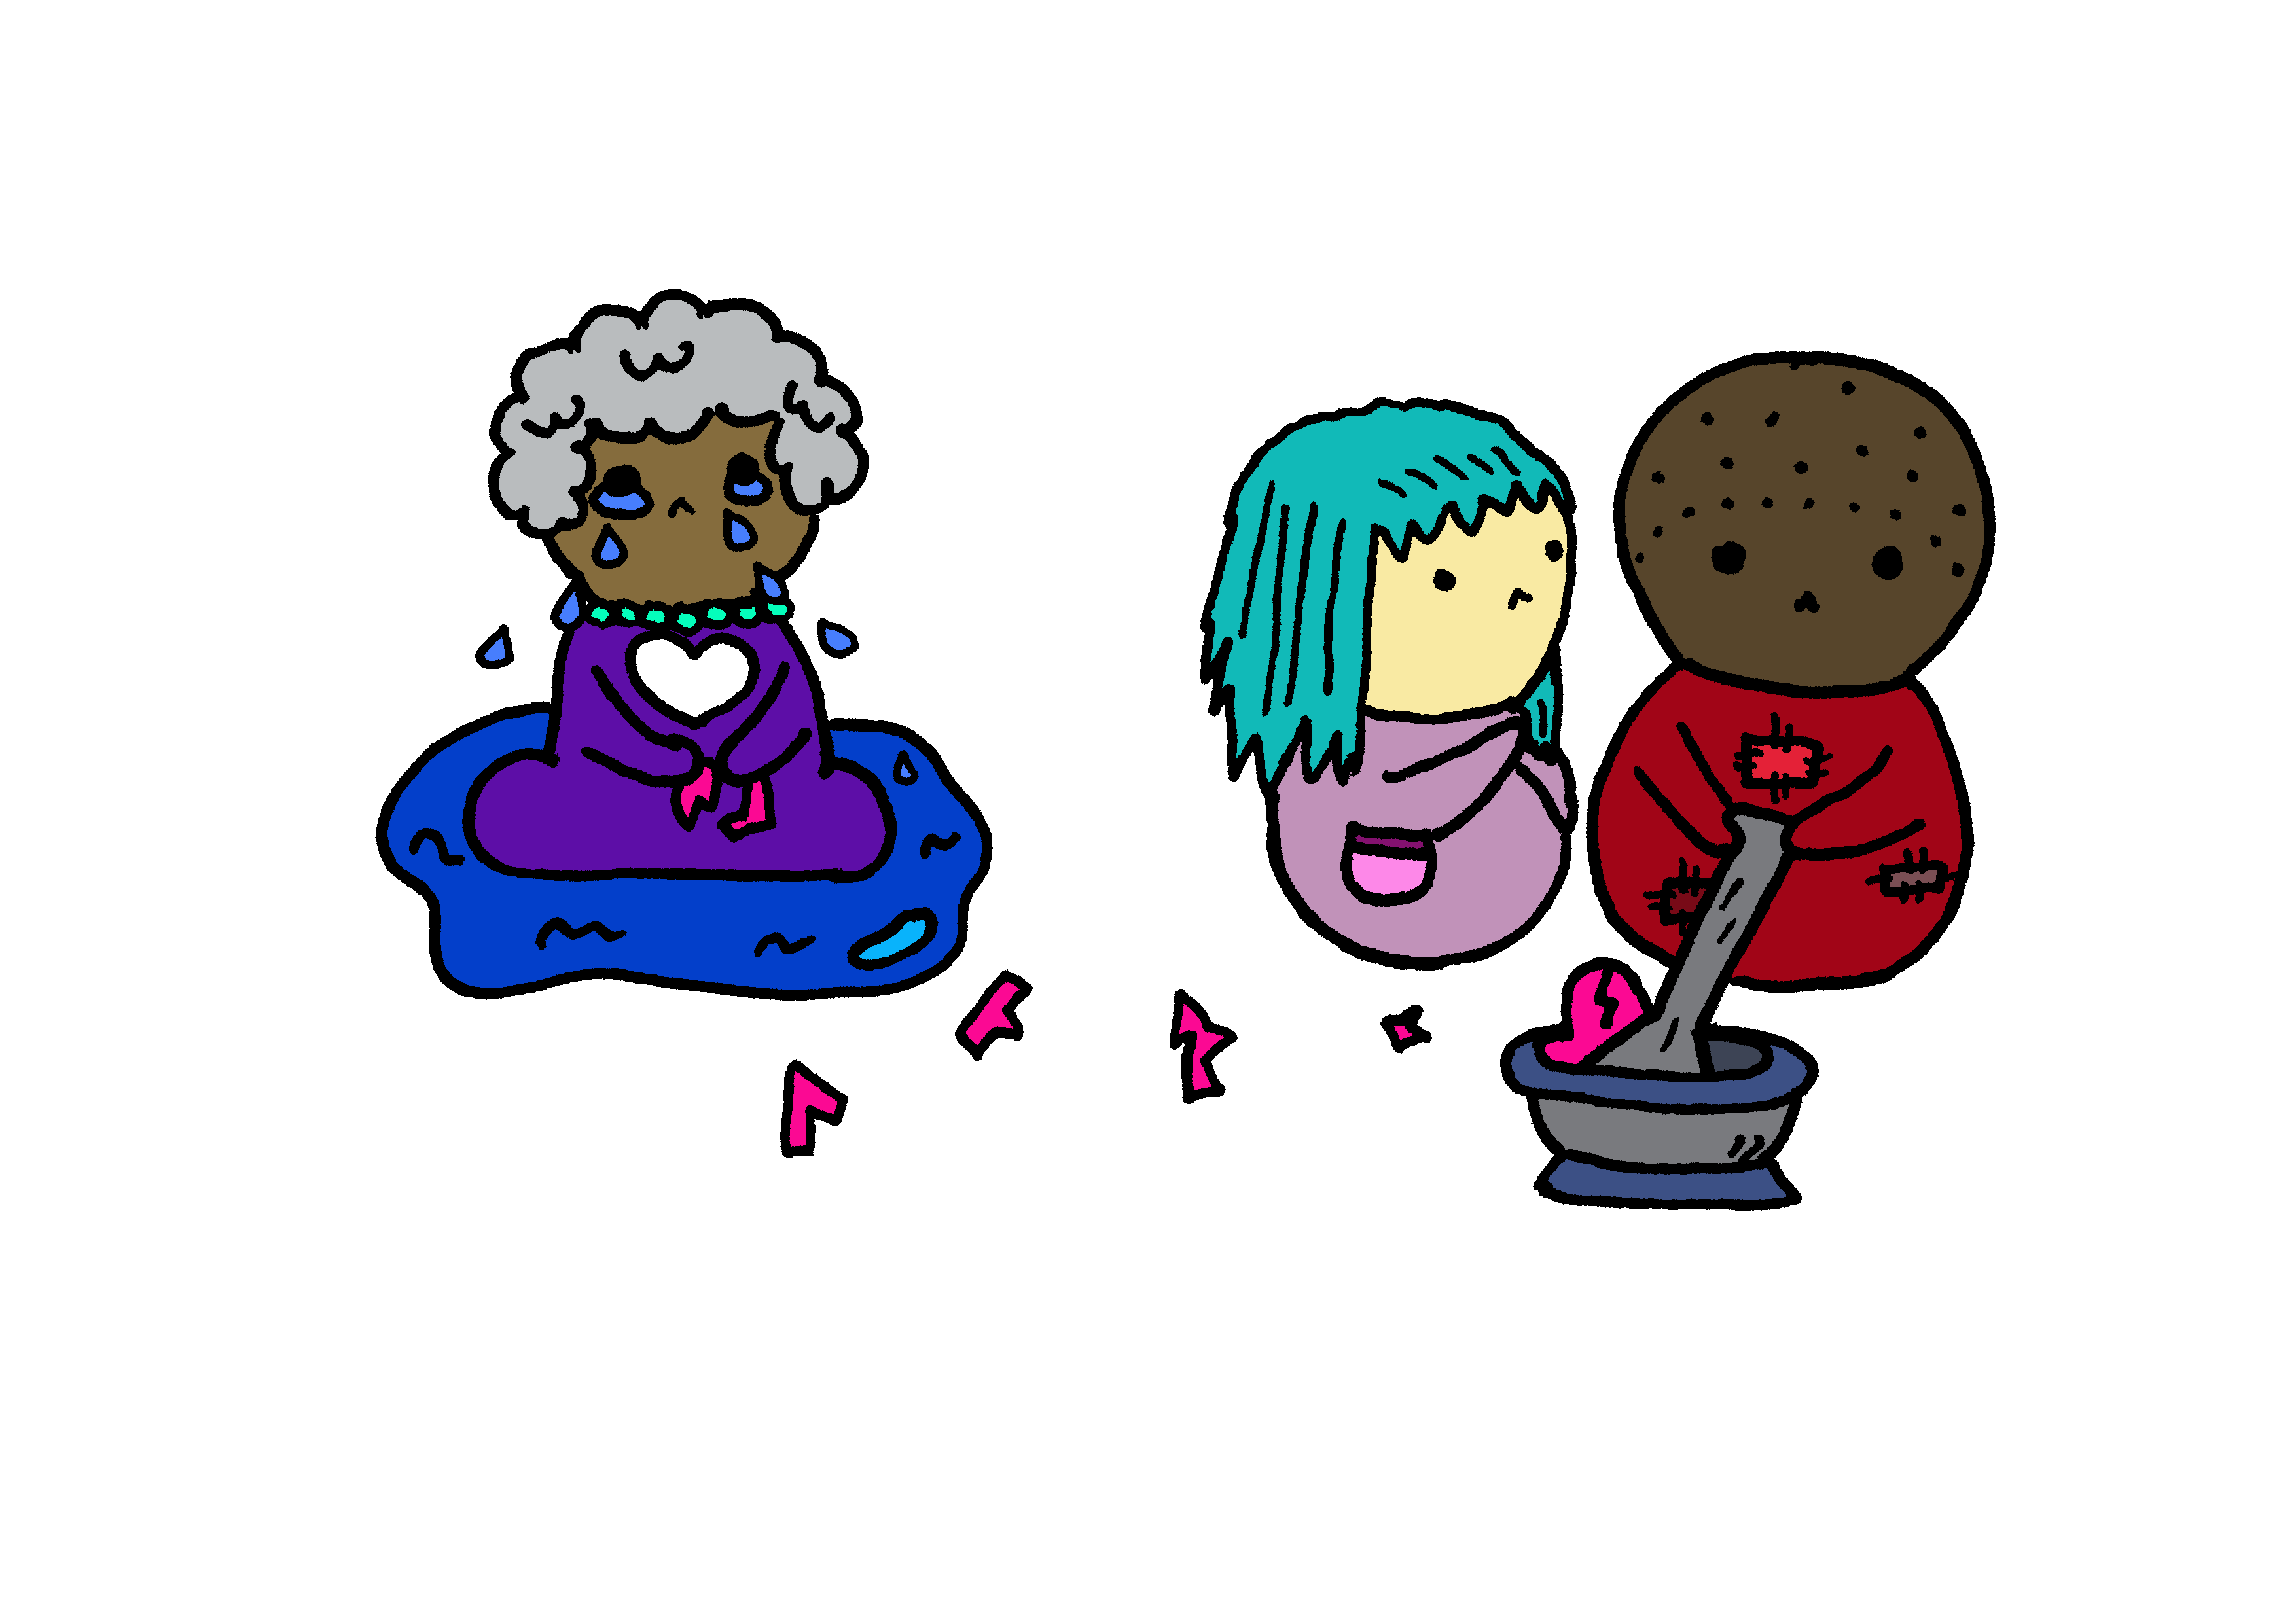
\includegraphics[width=0.5\paperwidth]{42.png}}
\end{figure}

\subsubsection*{La atención afirmativa de género}

La transición, también conocida como `atención afirmativa de género', sucede cuando alguien decide tomar los pasos necesarios para sentirse más alineade social y/o físicamente con su género. Es un proceso personal que una persona puede considerar necesario para poder vivir en la sociedad encarnando su identidad de género, y puede conllevar procedimientos sociales, médicos, quirúrgicos y legales. Esto no significa que una persona que transiciona está `cambiando de género', que `está cambiando de sexo' o que `se está convirtiendo en hombre o mujer'; alguien que decide transicionar, a través de dichos procesos, confirma el género que siempre tuvo. No existe tal cosa como una sola  `transición completa'; independientemente de la apariencia, documentos, hormonas o procedimientos quirúrgicos, cada quien podrá decidir cuándo acaba su transición.

No hemos de confundir el concepto de transicionar con identificarse como trans: algunas personas que deciden recibir dicha atención afirmativa se identifican como trans, mientras que otras se identifican simplemente como hombres o mujeres.

\subsubsection*{Transición social}

La transición social es el proceso mediante el cual una persona decide cambiar su expresión de género para que esté en armonía con su identidad de género, y puede conllevar salir del armario y declararse trans, cambiarse el nombre, el pronombre y la apariencia. Aquellas personas que decidan transicionar socialmente pueden también cambiar qué opción usar en los espacios separados por género, como los baños. Puede incluirse también el cambio de género en el pasaporte, certificado de nacimiento y otros documentos oficiales.

\subsubsection*{Transición física / corporal }

Una persona que decida llevar a cabo una transición física puede cambiar distintos elementos de su apariencia, como la ropa, el maquillaje y el cabello, para que estos se alineen con su identidad de género. También puede conllevar distintos tratamientos médicos, ya sea procedimientos quirúrgicos o la toma de hormonas. 

\begin{figure}[h]
    \centering
    \makebox[0pt]{%
    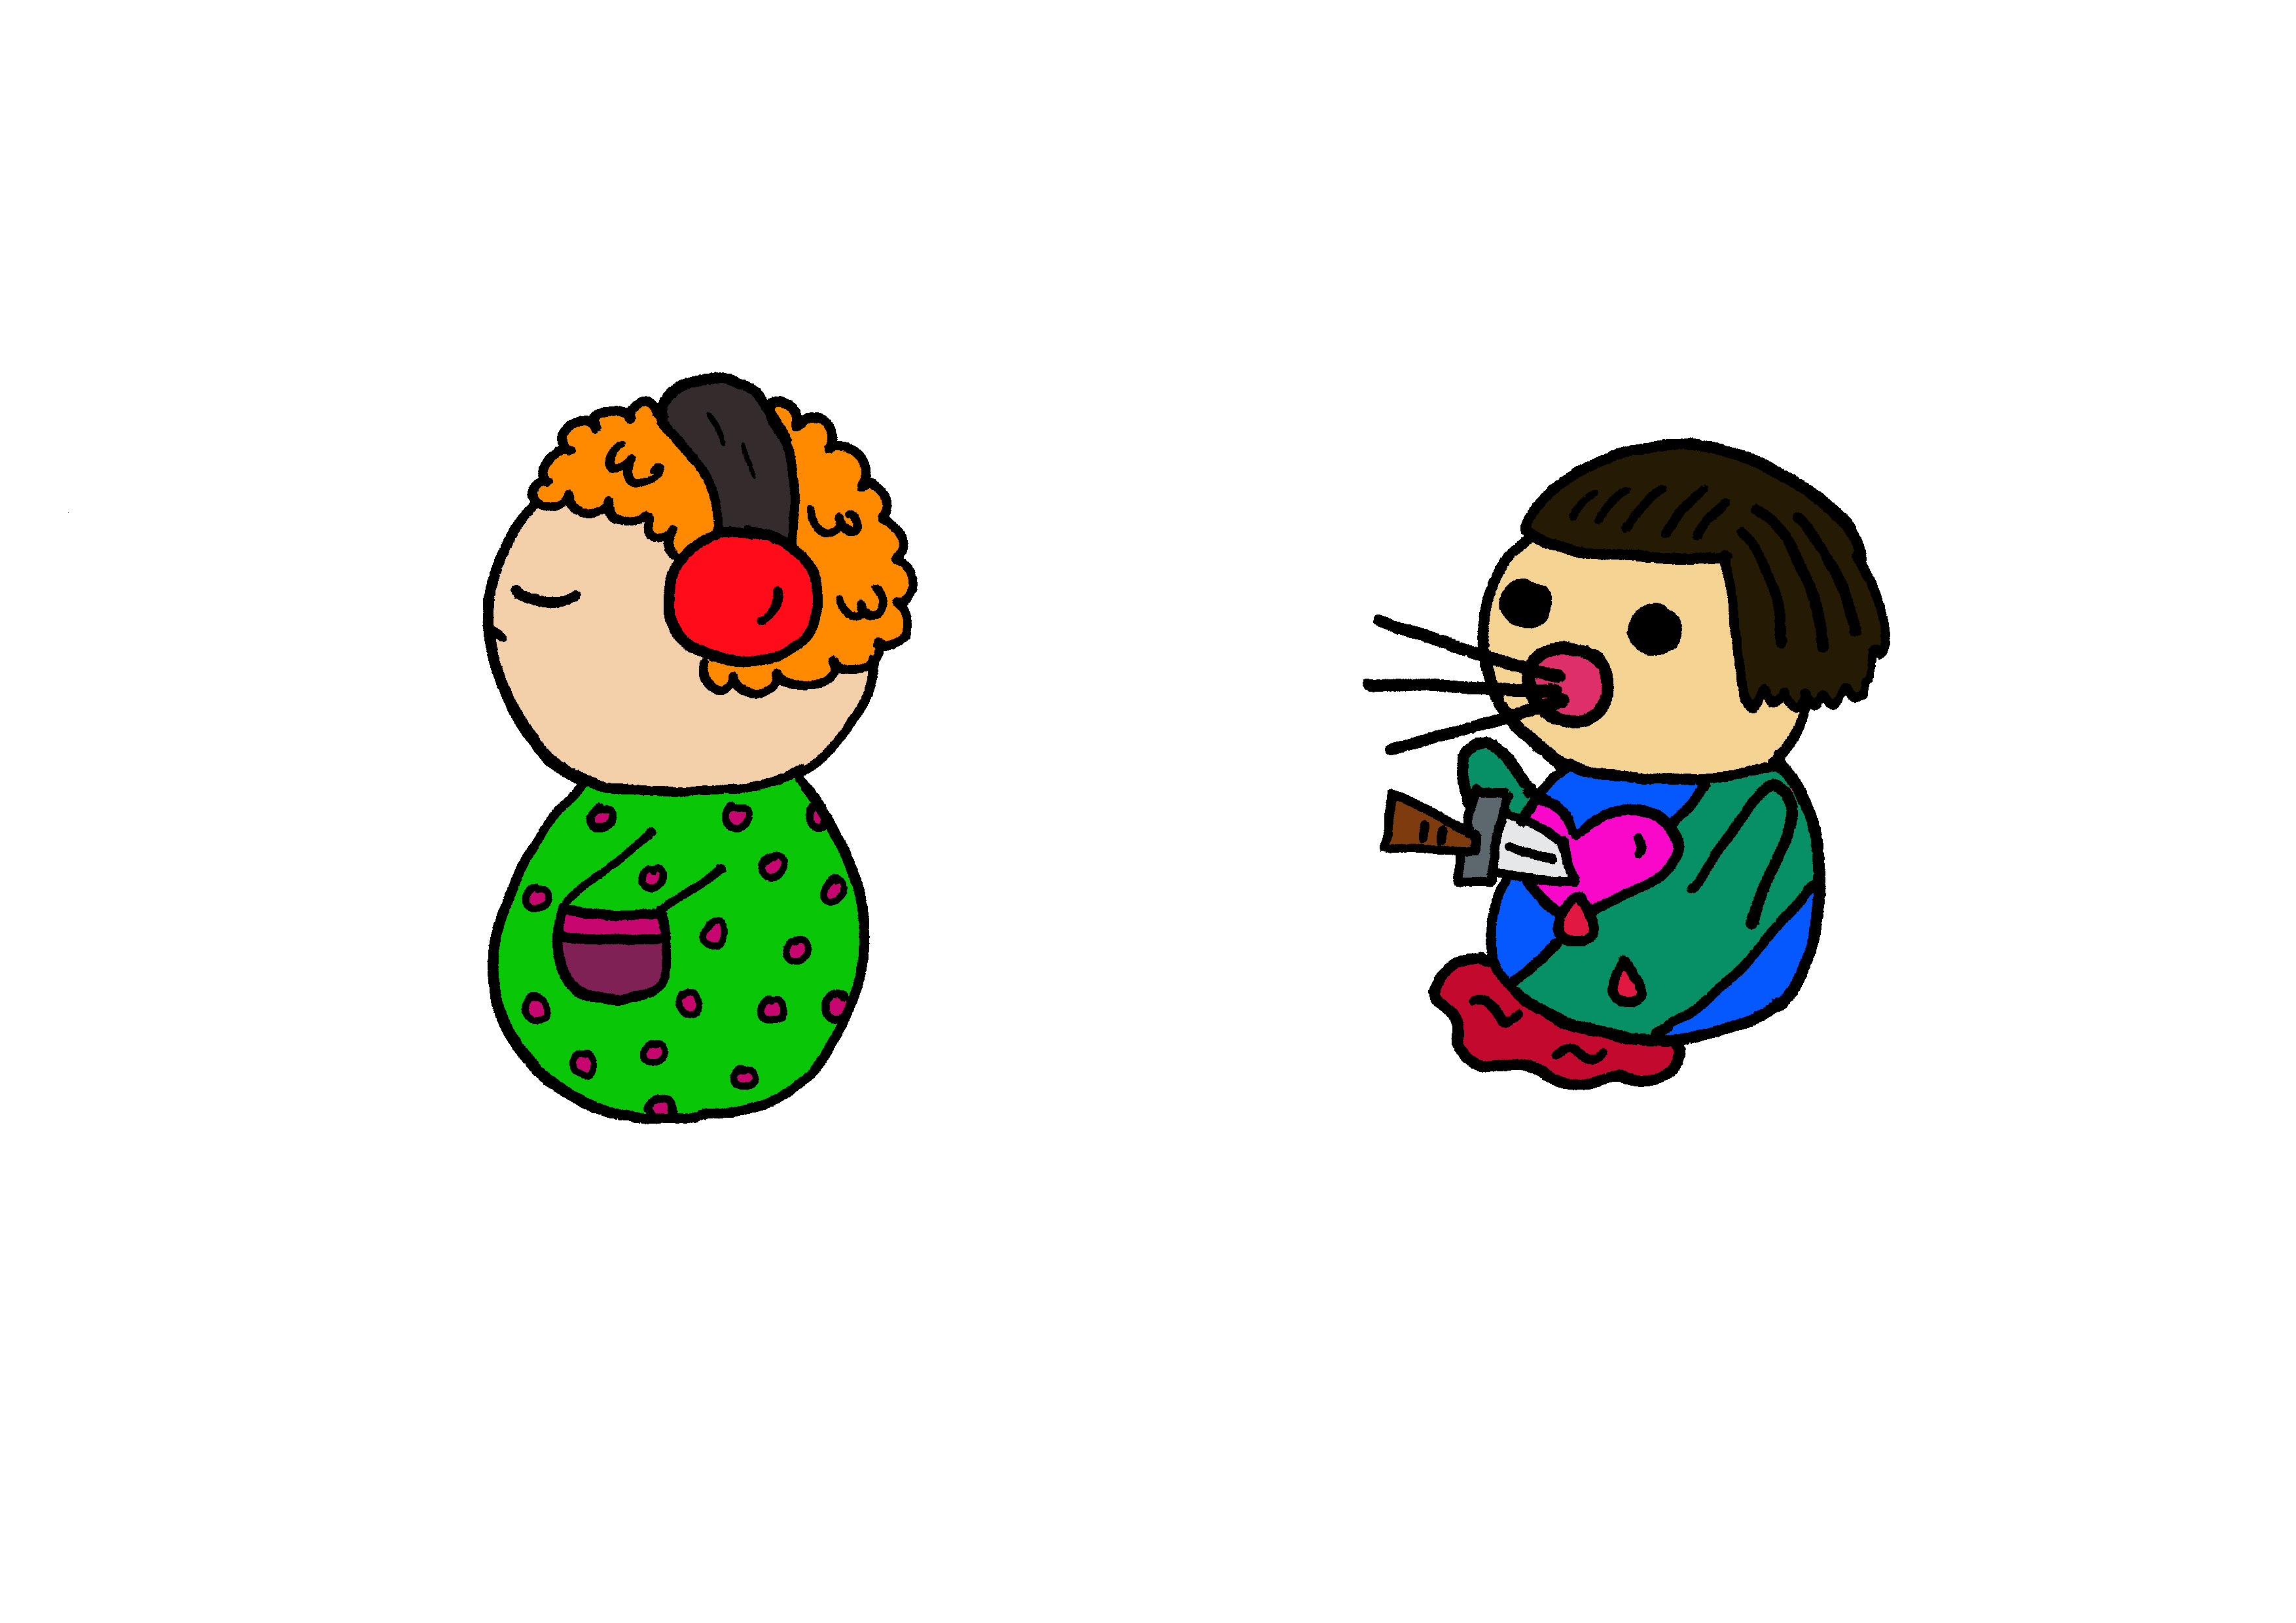
\includegraphics[width=0.5\paperwidth]{44.png}}
\end{figure}

\subsubsection*{No binarie}

El término `no binarie', también conocido como `NB', es un hipónimo de `trans', y se refiere al género de aquelles que no se identifican ni como hombres ni como mujeres. Puede, por ejemplo, que se identifiquen con algunos aspectos de ambos género binarios, que se identifiquen en el medio de dicho binario o que su género vaya más allá de esa construcción binaria. Une puede identificarse meramente como no binarie o usar este término como un hiperónimo que abarca muchos otros géneros no binarios, los cuales pueden ser, por ejemplo: género fluido (vivir el género en un espectro), transmasculine o transfemenine (vivir el género con tendencias a alguno de los géneros binarios), agénero (la carencia de un género) y bigénero (cuando une se identifica tanto como hombre como mujer). Estos términos, entre muchos otros, describen cómo las personas no binarias sienten y expresan su género. Muchas personas no binarias también se identifican como transgénero.

\newpage
\begin{figure}[h]
    \centering
    \makebox[0pt]{%
    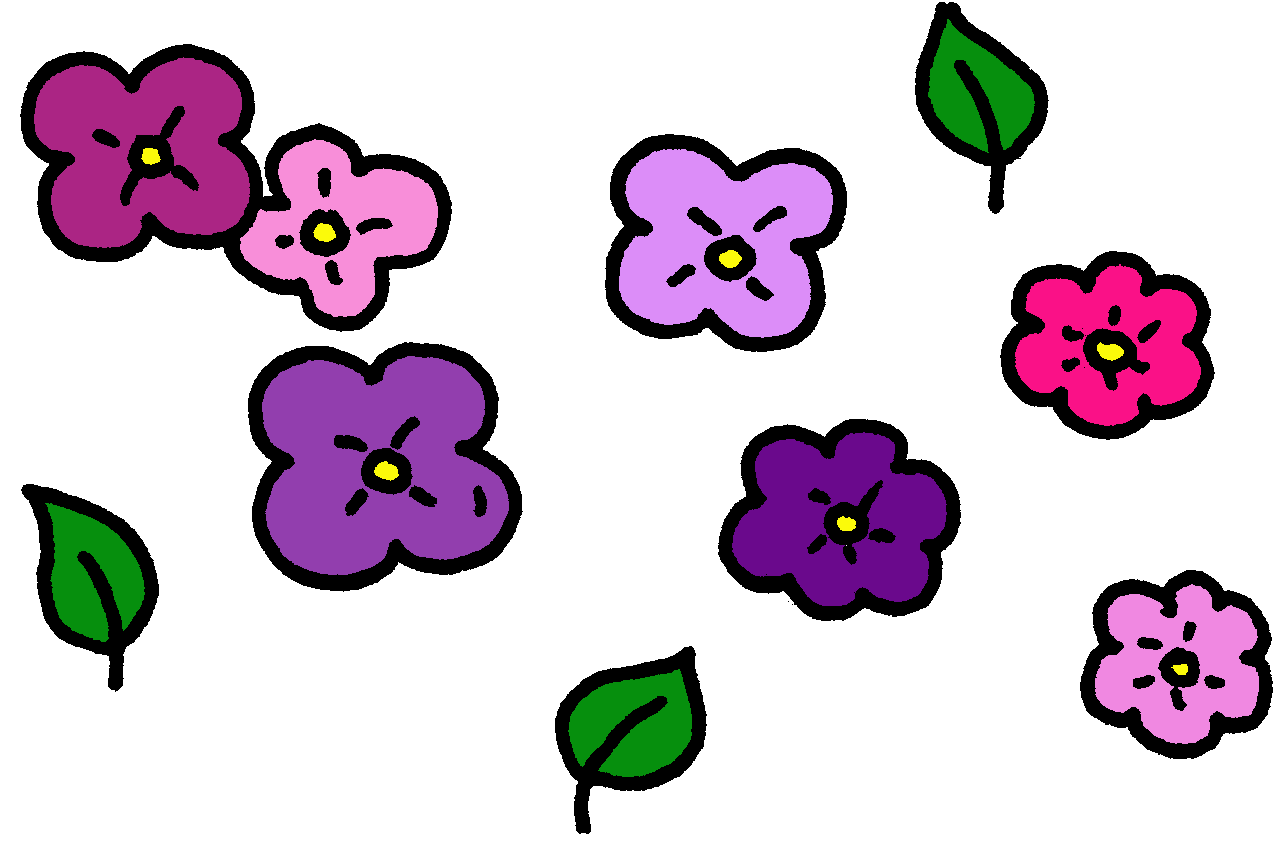
\includegraphics[width=0.5\paperwidth]{40c.png}}
\end{figure}

Identificarse como no binarie no es lo mismo a ser intersexual; las mayor parte de personas no binarias son asignadas `hombres' o `mujeres' al nacer, pero no se identifican como tal. No hay ninguna correlación entre la identidad no binaria y la orientación sexual, puesto que las personas no binarias tienen el mismo rango de orientaciones posibles como las personas binarias. Mientras que algunas personas no binarias decidan someterse a procedimientos quirúrgicos o tomar hormonas para sentirse más cómodes con sus cuerpos, otres deciden no someterse a ningún tratamiento médico ya que se sienten felices con sus cuerpos. Algunas personas no binarias deciden mostrarse como andrógines, pero otras se muestran como tradicionalmente masculines o femenines. Sin embargo, siguen siendo no binaries.

\medskip

\noindent\fbox{%
    \parbox{\textwidth}{%
\textit{\textbf{\Large \textcolor{white}{Comportamientos hirientes contra las personas trans y no binaries}}}

\medskip

\textcolor{white}{Existe la creencia de que las personas trans no existen, conocido como `cisexismo' o `cisgenerismo'. Además, las personas cisexistas afirman que existen únicamente identidades binarias (hombre o mujer) y que la identidad de género se restringe al sexo asignado al nacer y/o a las características sexuales.}

\textcolor{white}{La malgenerización sucede cuando nos referimos a alguien usando lenguaje que no va acorde a su identidad de género, como el uso incorrecto de pronombres (él, ella, elle…), las palabras referentes a la familia (padre, madre, tío, tía, hermano, hermana…), y otras palabras que han sido limitadas tradicionalmente a un género, como `guapo', `bonita'…}
 
\textcolor{white}{El término `transfobia' se refiere a los prejuicios y estereotipos de personas trans y de género diverso. La transfobia resulta en el uso de lenguaje irrespetuoso o peyorativo, la falta de respeto a la expresión de género de una persona (que incluye la vestimenta y el baño o alojamiento que se decida usar) y diversos tipos de violencia, como amenazas, acoso sexual, violencia física y la exclusión de una persona por su identidad de género.}
    }%
}

\phantomsection
\section*{Orientación sexual}
\addcontentsline{toc}{section}{Orientación sexual}

La orientación sexual (también conocida como `sexualidad') y el género son dos temas distintos: el género se refiere a la manera en que nos relacionamos con les demás (`hombre', `mujer', u otro género distinto), mientras que la orientación sexual se refiere hacia quiénes sentimos atracción. Una persona cisgénero puede ser gay, heterosexual, bisexual, asexual… De igual forma, una persona trans puede ser gay, heterosexual, bisexual, asexual…

\subsubsection*{Lesbiana}

Este término hace referencia a una mujer a quien le atrae otras mujeres de forma sexual y/o romántica.

\subsubsection*{Gay}

Este término hace referencia a un hombre a quien le atrae otros hombres de forma sexual y/o romántica. Las mujeres que se sienten atraídas sexual y/o románticamente a otras mujeres también se pueden referir a sí mismas como `gay'.

\subsubsection*{Queer}

Este término alude a un amplio espectro de orientaciones sexuales e identidades de género. A pesar de haberse usado como una palabra peyorativa en sus orígenes en el idioma inglés, la palabra `queer' ha sido reapropiada y es utilizada para describir a la gran variedad de identidades LGBTQIA+.

\subsubsection*{Bisexual}

El término `bisexual' se refiere a aquellas personas que se sienten atraídas romántica y/o sexualmente a personas de su mismo género y a personas de otro género. Cabe recalcar que la bisexualidad no implica que existan solamente dos géneros; se ha creado el término `pansexual' para referirse a la atracción sin restricciones de género, incluyendo así a las personas trans y no binarias.

\subsubsection*{Heterosexual}

El termino `heterosexual' se refiere a aquellas personas que se sienten atraídas sexual y/o románticamente por el sexo opuesto.

\subsubsection*{Orientación Romántica}

La orientación romántica describe por quién nos sentimos atraídos románticamente, y puede ser distinta a nuestra orientación sexual. Las orientaciones románticas funcionan de manera muy similar a las orientaciones sexuales y describen los géneros que le interesen a alguien de manera romántica.

\subsubsection*{Asexual}

La orientacion `asexual' se define como la falta de atracción sexual, ya sea dentro o fuera de las relaciones sociales. Les asexuales pueden experimentar atracción romántica en todo el espectro LGBTQIA+ y participar en actividades sexuales a pesar de no sentir atracción sexual. Comportamientos dañinos hacia las personas atraídas por personas del mismo sexo.

\bigskip

\noindent\fbox{%
    \parbox{\textwidth}{%
\textit{\textbf{\Large \textcolor{white}{Comportamientos dañinos hacia las personas atraídas por personas del mismo sexo}}}

\bigskip

\textcolor{white}{\textbf{Bifobia}: La bifobia es una actitud dañina hacia alguien que se siente atraído por más de un género. Puede incluir decirle a alguien que su sexualidad es `solo una fase' o que `elija un bando'. Etiquetar a los bisexuales como homosexuales o heterosexuales al estar en una determinada relación borra su verdadera identidad bisexual.}

\medskip

\textcolor{white}{\textbf{Heteronormatividad}: La heteronormatividad es la visión errónea de que las relaciones heterosexuales son las únicas expresiones naturales, normales y legítimas de la sexualidad y de relaciones interpersonales; que otras sexualidades o identidades de género no son naturales y representan una amenaza para la sociedad.}

\medskip

\textcolor{white}{\textbf{Homofobia}: La homofobia conlleva creencias negativas, prejuicios y estereotipos en contra de personas no heterosexuales. Su expresión verbal es común, como los insultos, chismes y palabras peyorativas (como `maricón' o `tortillera') o frases como `eso es de maricones'. La homofobia también puede expresarse como amenazas abusivas, violencia física, acoso sexual, legislación discriminatoria y exclusión deliberada de alguien por su sexualidad.}
    }%
}

\newpage
\textbf{Más información: }https://rainbodhi.org/resources/

\medskip

{\footnotesize
\begin{center}
\noindent \textbf{Edición original 2021:}

This booklet was produced by LGBTQIA+ Buddhists. All identity groups in the rainbow acronym were consulted for input and feedback.

\noindent Many thanks to Venerable Vimala, Ayya Vimalanyani, Bhante Sumano, Erland Moeckli, JJ, Nilushi Disayanake, Letty, all the Rainbodhi crew, the Buddhist Council of NSW, GiveOUT Day Australia, Simone Ford, Bronwyn Sweeney and a special thanks to all the many people who donated funds to produce this booklet.

\medskip

\noindent First Published in Australia 2021 by MegaCity Books for Rainbodhi LGBTQIA+ Buddhist Community

\smallskip


\includegraphics{by-nc-sa}

\noindent This work is created under a Creative Commons Attribution-NonCommercial-ShareAlike 4.0 International License

\noindent A catalogue record for this book is available from the National Library of Australia.

\medskip

\noindent ISBN: I978-0-64889593-1-1

\medskip

Author: Akaliko Bhikkhu \\
Illustrator: Venerable Yodha \\
Contributor: Letty \\
Project management and design: Kerry Klinner, megacitydesign.com \\
Editor: Simone Ford \\
Proofreader: Bronwyn Sweeney

\bigskip

\textbf{Edición en español 2023:}  \\
Traducción: Grégory Touche (Ngakpa Padma Özer), Ngakpa Alan Serrato Martínez (Tenzin Dradul) \\
Corrección: David Santamarina (Kansei) \\
Ilustraciones: Venerable Yodha \\
Formato y diseño: Remy Jakobson, Venerable Vimala
\end{center}
}

\newgeometry{margin=0pt}

\begin{figure}[ht]
    \centering
    \makebox[0pt]{%
    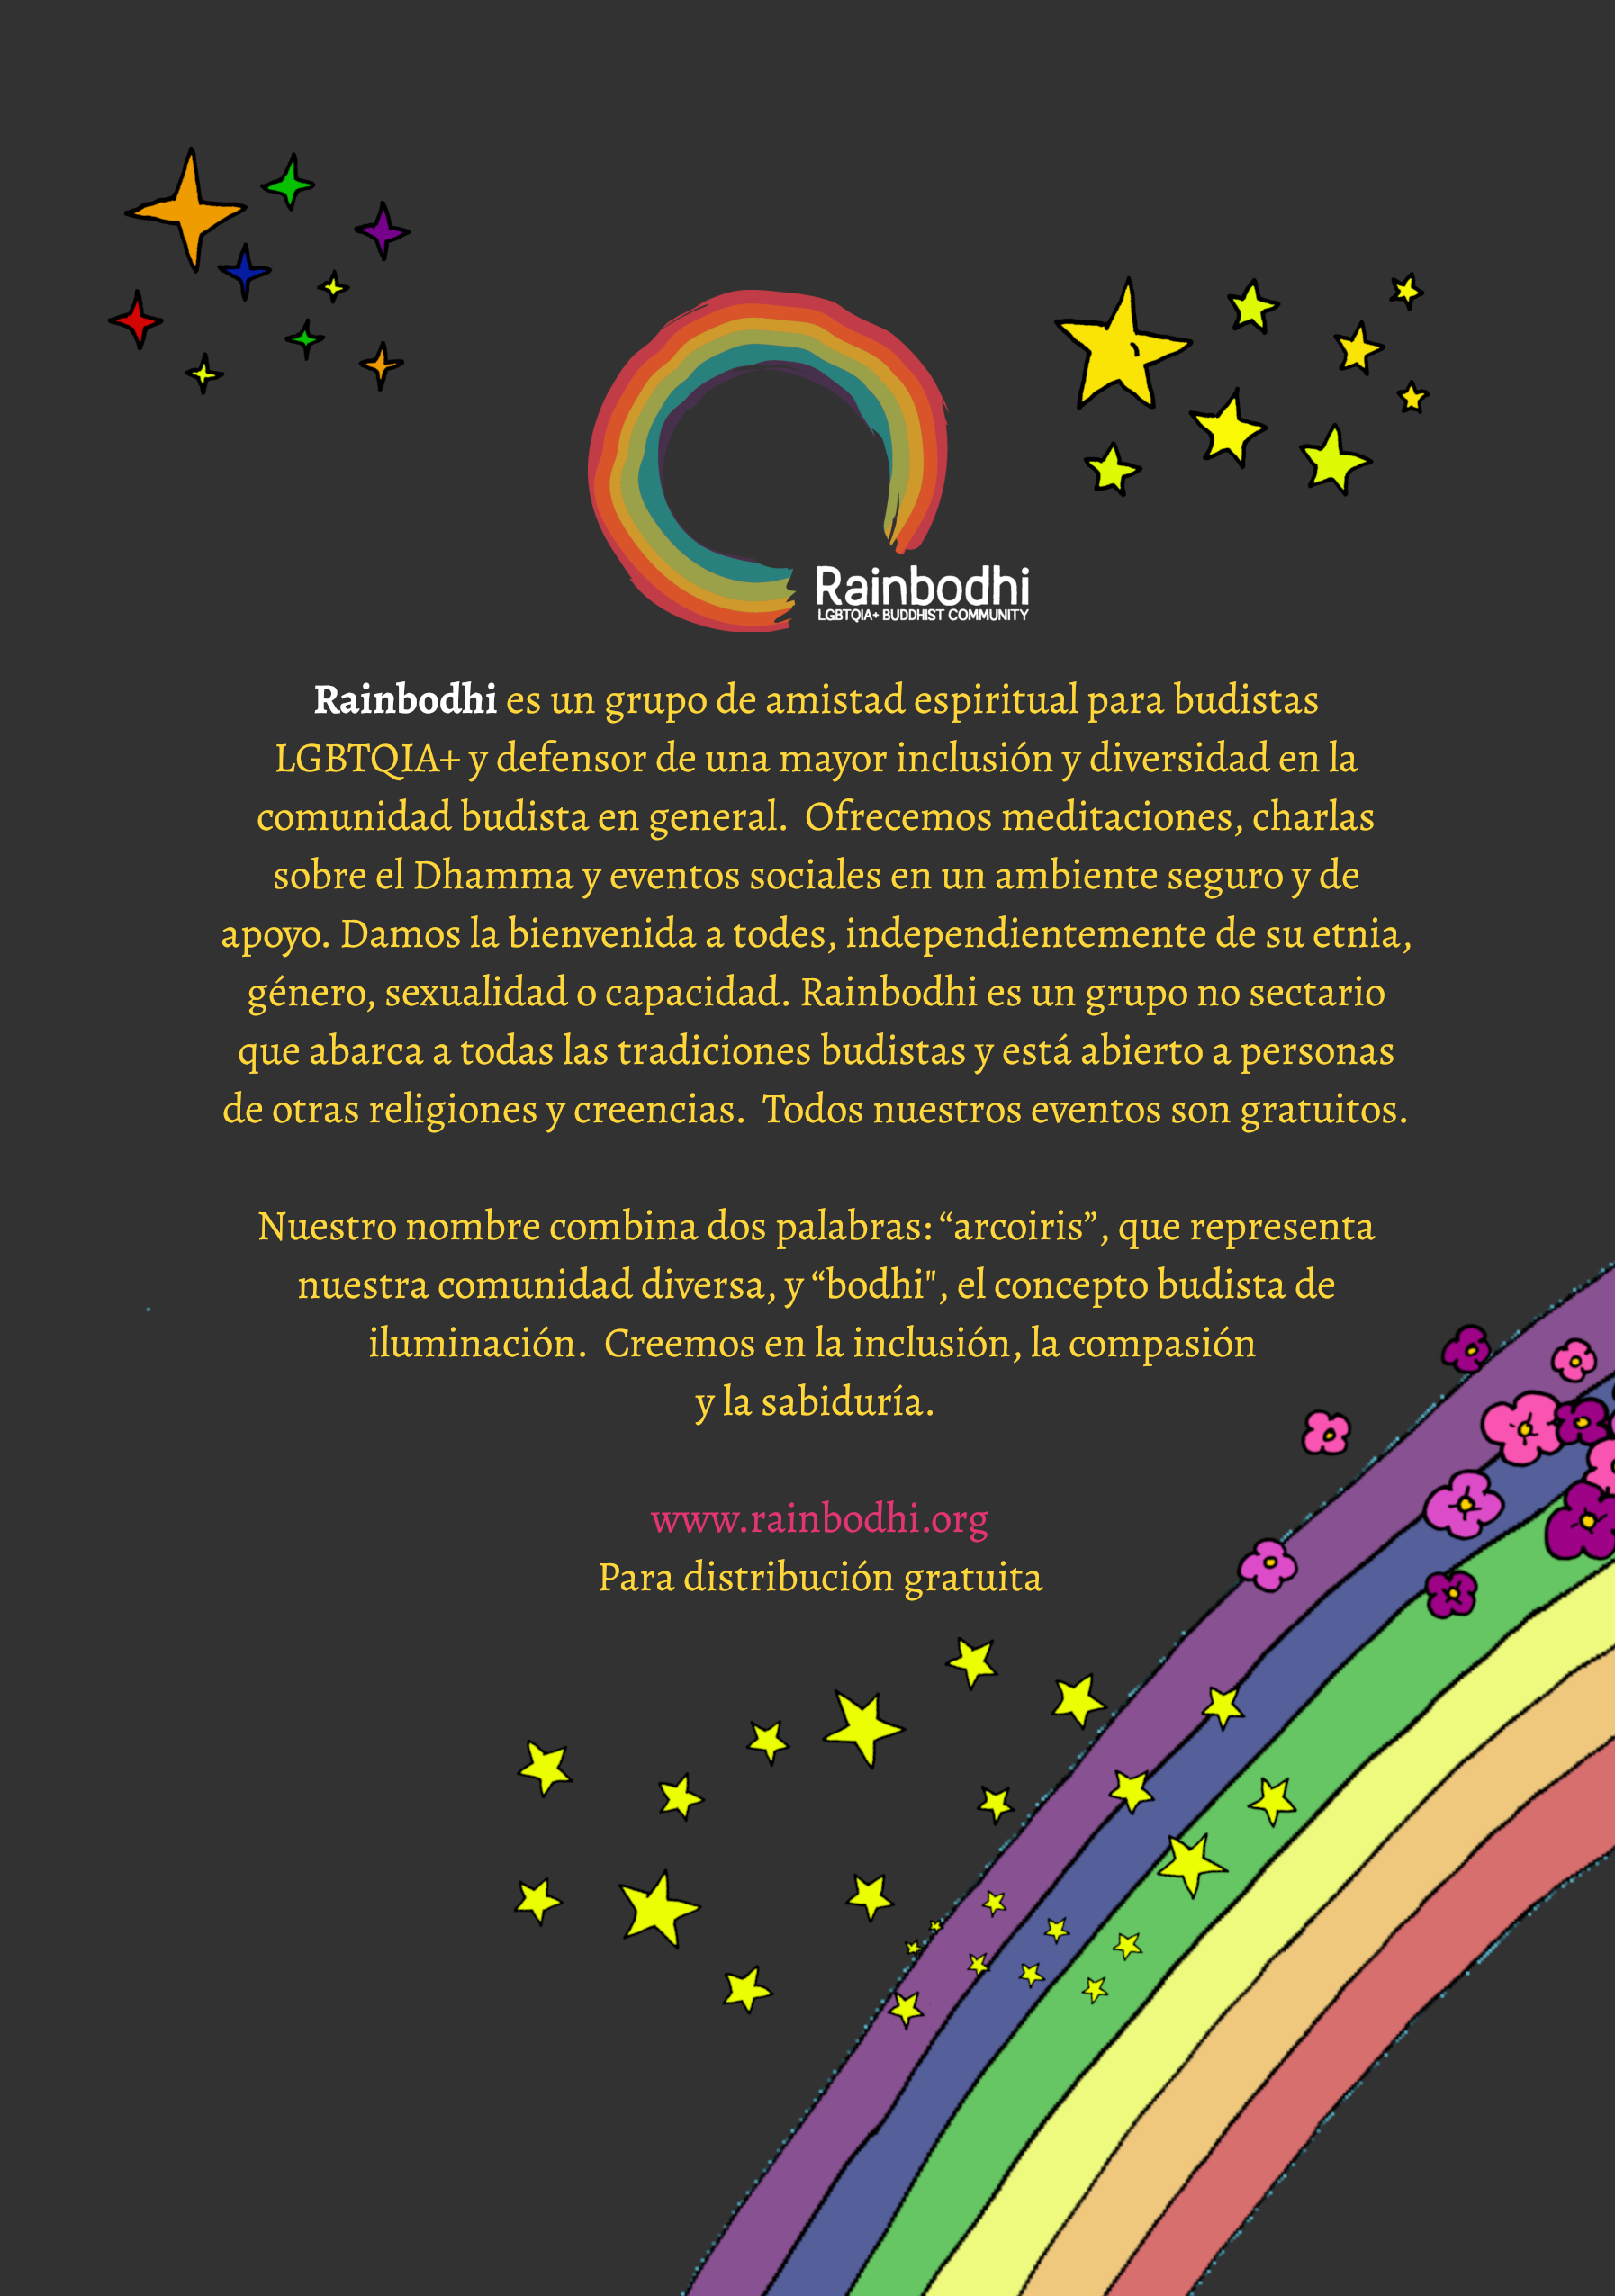
\includegraphics[width=\paperwidth]{back_espanol.png}}
\end{figure}

\end{document}